% notes can be: hide, only or show
\documentclass[ignorenonframetext,red,8pt,notes=hide]{beamer}

\usepackage[utf8]{inputenc}
\usepackage{beamerthemesplit}
\usepackage{graphics}
\usepackage{natbib}
\usepackage[english]{babel}
\usepackage{url}
\usepackage{times}
\usepackage[T1]{fontenc}
\usepackage{hyperref}
\usepackage{epstopdf}
\usepackage{subfig}

\usepackage{multirow}
\usepackage{rotating}

\usepackage{booktabs}


% hack for beamer and natbib working together
%\newcommand{\newblock}{}

\mode<presentation>
{
	\usetheme{Warsaw}
    % remove sections and subsections form each slide
    \setbeamertemplate{headline}{}
    %\setbeamertemplate{headline}{\vspace{0.05cm}}
    % center frame titles
    \setbeamertemplate{frametitle}[default][center]
    % remove navigation buttons
    \beamertemplatenavigationsymbolsempty
% 	\usecolortheme{lily}
}

\mode<article>
{
  \usepackage{fullpage}
  \usepackage{pgf}
%  \setjobnamebeamerversion{beamerexample2.beamer}
}

\usepackage{fancyvrb}
\usepackage{color}
%\usepackage{colortbl}
\usepackage{listings}
%\usepackage{listings,bera}
\definecolor{keywords}{RGB}{128,148,182}
%\definecolor{comments}{RGB}{60,179,113}
\definecolor{comments}{RGB}{0,0,139}
\lstset{language=Python,
        %numbers=false,
        showstringspaces=false,
        numberstyle=\tiny,
        %frame=leftline,
        numbersep=4.5pt,
  keywordstyle=\color{keywords}\bfseries,
  commentstyle=\color{comments}\emph
}

\hypersetup{
%   pdfpagemode=FullScreen, % Sembla que no funciona correctament
  unicode=true,
  pdftitle={The Structural Dimension of Cooperation},%
  pdfauthor={Jordi Torrents},%
  pdfcreator={},%
  pdfproducer=PDFLaTeX,%
  pdfsubject={},%
  pdfkeywords={}%
}

%\AtBeginSection[]{\frame{\frametitle{Contents}\tableofcontents[current]}}

\title[Analyzing code contributions to the CPython project]{Analyzing code contributions to the CPython project using NetworkX and Matplotlib}
\subtitle{PyData Barcelona 2017}
\author{Jordi Torrents\\ jordi.t21@gmail.com}
\institute{Department of Sociology\\University of Barcelona}

\begin{document}

\begin{frame}[label=portada]
\maketitle
\end{frame}

\begin{frame}[label=toc]
\frametitle{Contents}
\tableofcontents
\end{frame}

\section{Large Scale Cooperation}

\subsection{Theoretical Approaches to Cooperation}
\begin{frame}[label=]
\frametitle{Theoretical Approaches to Cooperation}

\begin{columns}[c]
\begin{column}{0.5\textwidth}

\begin{block}{Macro level approach}
Cooperation as a macro level phenomenon in which the center of analysis is the collective or group \citep{marx:1990, adler:2006, adler:2015}.

\begin{itemize}

\item Focus on large organizations and groups: Collaborative Communities

\begin{itemize}

\item Shared values and goals
\item Generalized trust
\item Authority forms

\end{itemize}
\end{itemize}
\end{block}
\end{column}

\pause

\begin{column}{0.5\textwidth}

\begin{block}{Micro level approach}
Cooperation as a micro level phenomenon in which the center of analysis is the dyad \citep{axelrod1981, watts:1999, eguiluz:2005}.

\begin{itemize}

\item Reductionist approach: Cooperation as an atomic process.

\begin{itemize}

\item Strategic dyadic interactions.
\item Agent-based models.
\item Payoffs of different strategies.

\end{itemize}
\end{itemize}

\end{block}

\end{column}
\end{columns}

\pause

\begin{block}{A Meso level approach to Cooperation}
Focus on Cooperation networks: patterns of relations that direct producers establish in the production process.
\begin{itemize}

\item Structural approach, that is, a network approach.

\begin{itemize}

\item Sub-groups that are more connected internally than with the rest of the network. 
\item Longitudinal analysis of the formation and dissolution of these groups.
\item Key mechanisms to explain and understand large scale cooperation.

\end{itemize}
\end{itemize}
\end{block}

\end{frame}


\section{Cohesive Groups: The Structural Cohesion Model}


\begin{frame}[label=]
\frametitle{Group Cohesion in the sociological literature}

Central concept that has a long and illustrious history in sociology. Its use in most sociological research has been ambiguous at best \citep{moody:2003}: 

\begin{enumerate}

\item sloppy definitions of cohesion with lack of generality.

\item grounded mostly in intuition and common sense.

\end{enumerate}

\begin{block}{Group cohesion \citep{doreian:1998} can be divided analytically into:}

\begin{description}

\item[Ideational component] based on the members' identification with a collectivity.

\item[Relational component] based on the patterns of connections among members.

\end{description}

\end{block}

\pause

The relational component of group cohesion has been the focus of Social Network Analysis.

\begin{block}{Network theory measures used to define group cohesion}

\begin{description}

\item[Classical measures] cliques, clans, clubs, $k$-cores, lambda sets, ...

\item[Community algorithms] detect groups of nodes more densely connected among them than with the rest of the network.

\end{description}

\end{block}

Neither the classical approaches nor new developments in community analysis work well in empirical analysis of group cohesion.

\end{frame}


\subsection{Key properties of cohesion measures}

\begin{frame}[label=]
\frametitle{Key properties that a cohesion measures should have}

\begin{columns}[c]
\begin{column}{0.3\textwidth}
\textbf{Robustness} its qualification as a group should not be dependent on the actions of a single individual.

\begin{center}
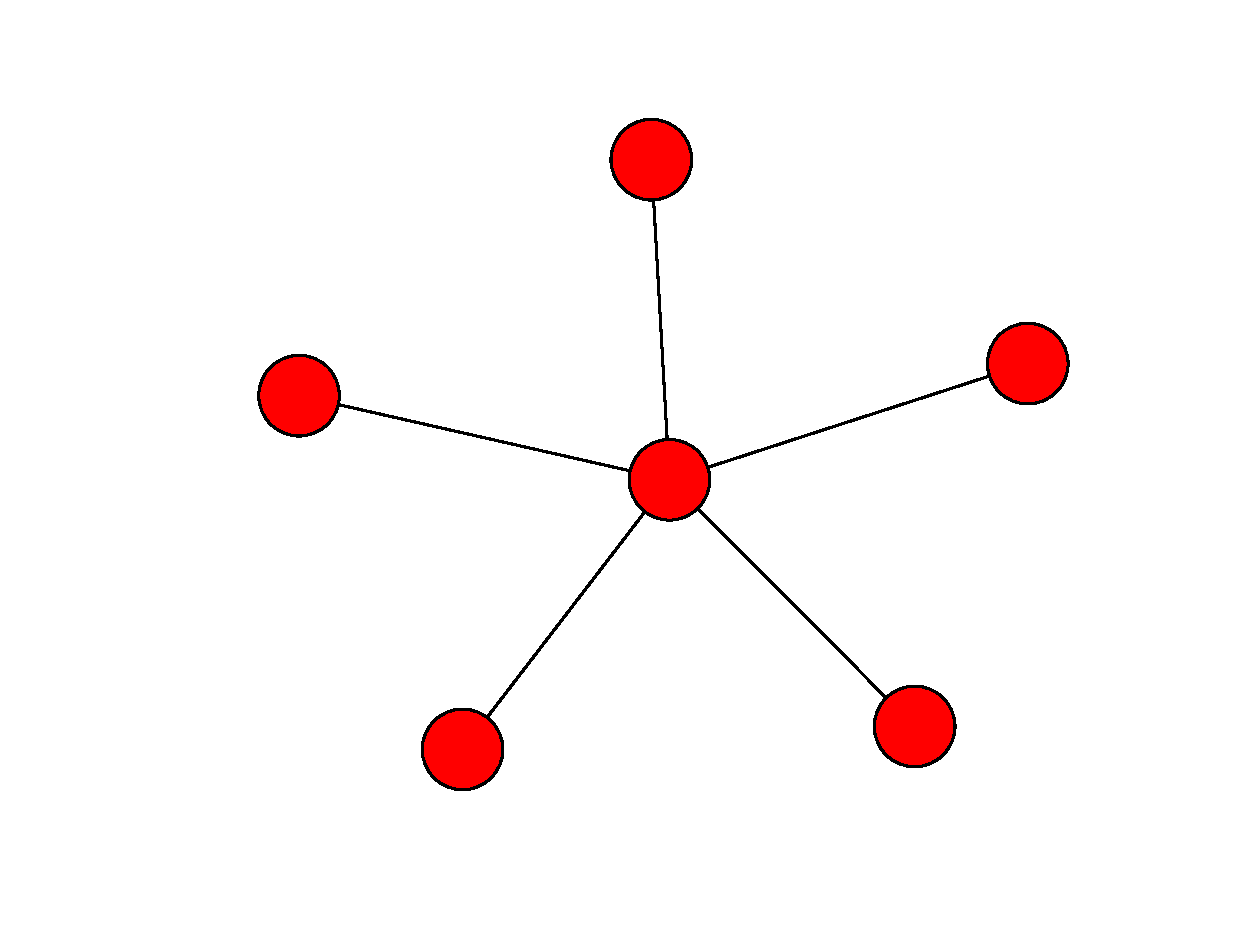
\includegraphics[scale=0.1]{img/star}
\end{center}

\begin{center}
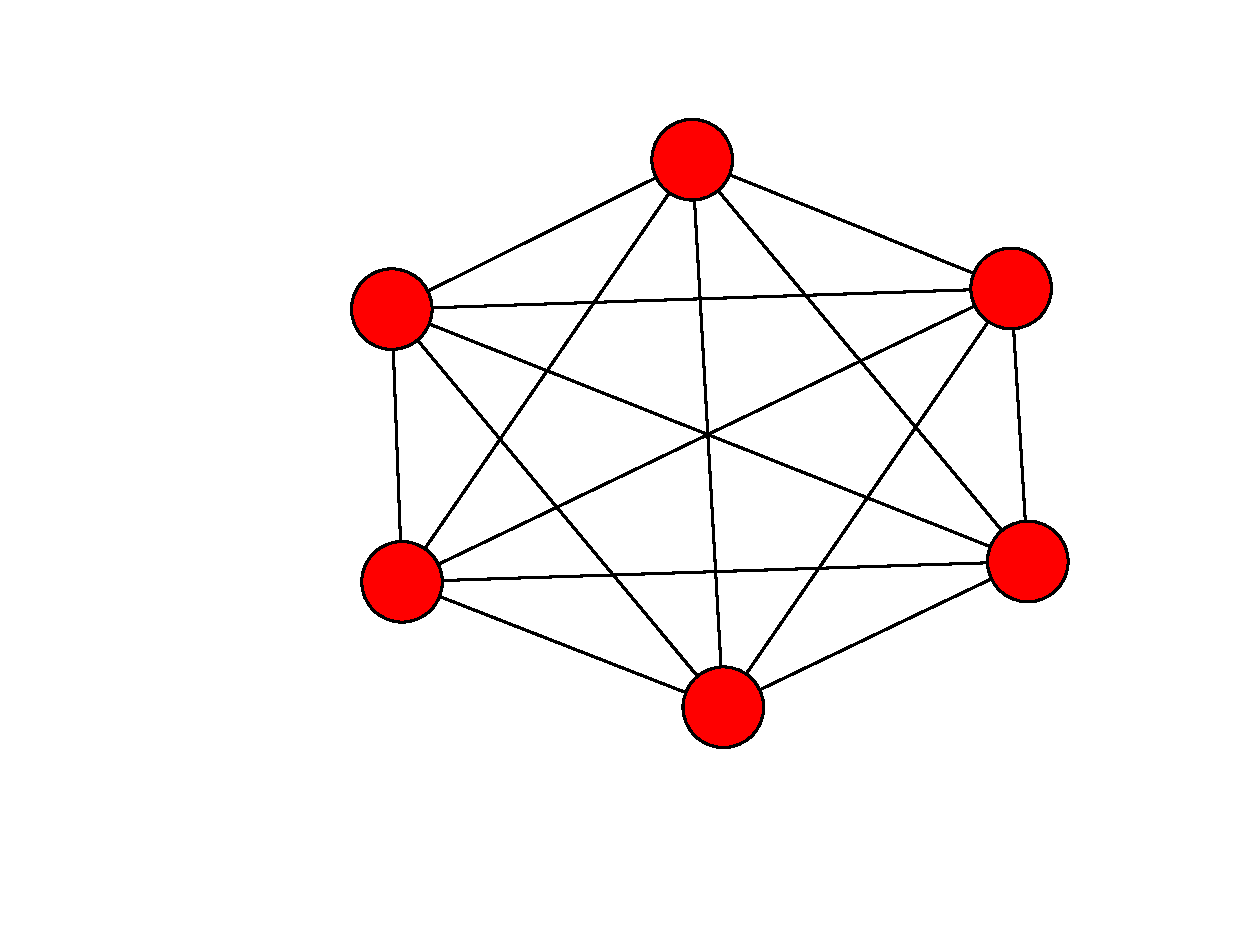
\includegraphics[scale=0.1]{img/complete}
\end{center}
\end{column}

\pause

\begin{column}{0.3\textwidth}
\textbf{Overlap} a cohesion measure should allow some actors to be part of more than one cohesive subgroup.

\begin{center}
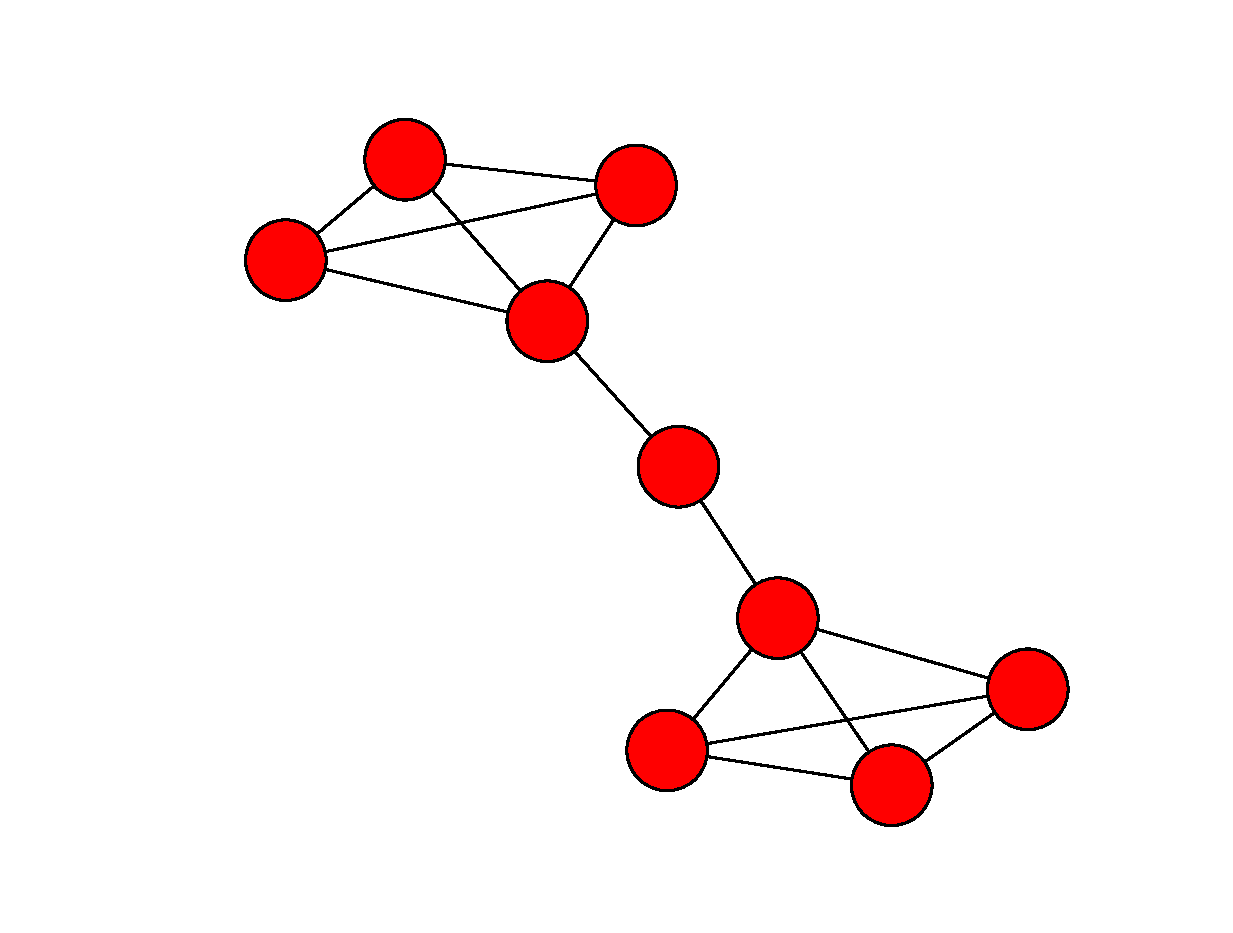
\includegraphics[scale=0.1]{img/hole}
\end{center}

\begin{center}
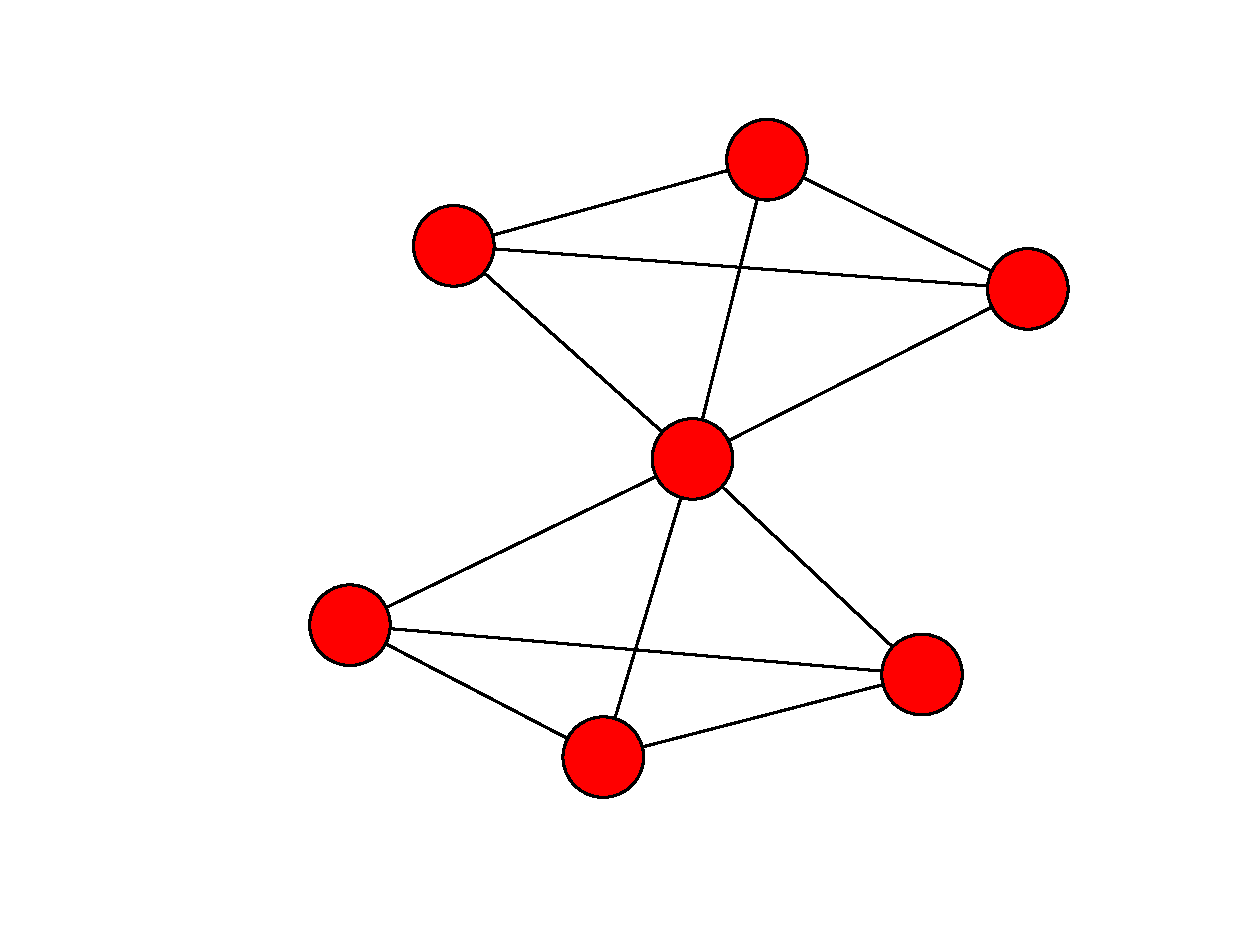
\includegraphics[scale=0.1]{img/fold}
\end{center}
\end{column}

\pause

\begin{column}{0.4\textwidth}
\textbf{Hierarchical} highly cohesive subgroups are nested inside less cohesive ones.

\begin{center}
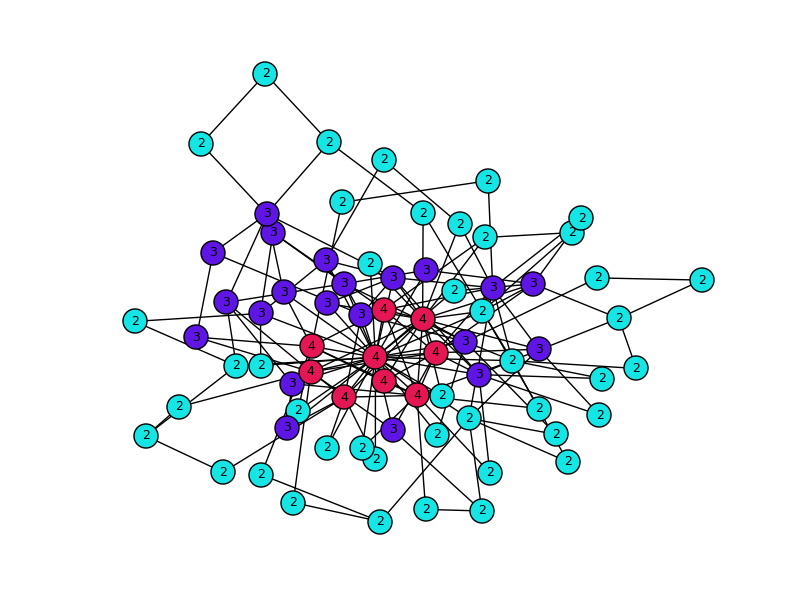
\includegraphics[scale=0.25]{img/knum_colors}
\end{center}
\end{column}

\end{columns}

\end{frame}

\subsection{Structural cohesion model}

\begin{frame}
\frametitle{The structural cohesion model}

The structural cohesion model \citep{white:2001,moody:2003} is based on two mathematically equivalent definitions of cohesion.

\begin{block}{Precise definition of group cohesion based on \textbf{node connectivity}}

\begin{itemize}

\item a group's structural cohesion is equal to the minimum number of actors who, if removed from the group, would disconnect the group.

\item a group's structural cohesion is equal to the minimum number of node independent paths linking each pair of actors in the group.

\end{itemize}
\end{block}

This equivalence relation has a deep sociological meaning because it allows to define structural cohesion in terms of:

\begin{itemize}

\item the difficulty to pull a group apart by removing actors.

\item multiple relations between actors that keep a group together.

\end{itemize}
\end{frame}

\begin{frame}
\frametitle{Components and $k$-components}

\begin{block}{Component}
A \emph{component} of a graph $G$ is a maximal connected subgraph, which means that there is at least one path between any two nodes in that subgraph.
\end{block}

\begin{block}{$k$-components}
A $k$-component is a maximal subgraph that has, at least, node connectivity $k$: we need to remove at least $k$ nodes to break it into more components. 
\end{block}

\begin{columns}[c]
\begin{column}{0.4\textwidth}
\begin{center}
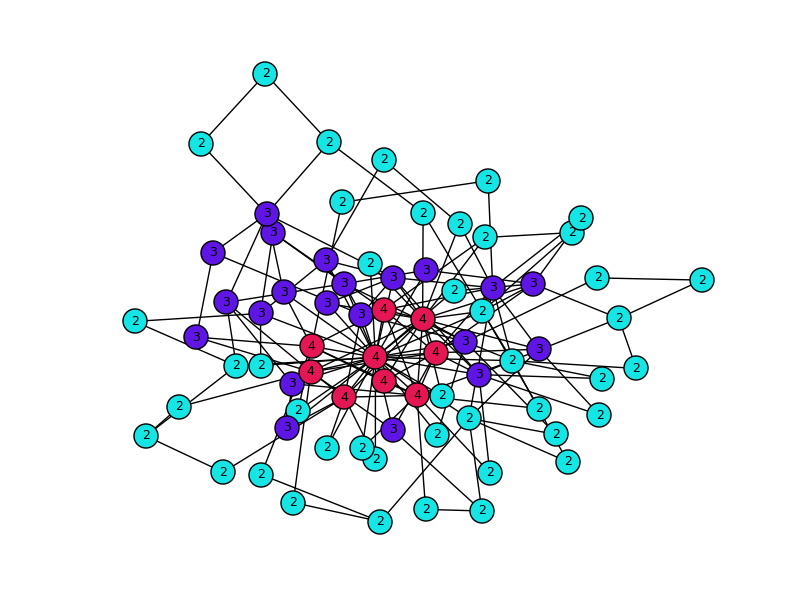
\includegraphics[scale=0.25]{img/knum_colors}
\end{center}
\end{column}

\begin{column}{0.6\textwidth}
\begin{itemize}
\item \textbf{Red Nodes} form a 4-component: we need to remove 4 nodes to disconnect it.
\item \textbf{Purple Nodes} form a 3-component along with red nodes: we need to remove 3 nodes to disconnect it.
\item \textbf{Blue Nodes} form a 2-component along with red and purple nodes: we need to remove 2 nodes to disconnect it. 
\end{itemize}
\end{column}
\end{columns}

\end{frame}


\section{Empirical analysis: FOSS projects}

\subsection{The CPython project}

\begin{frame}
\frametitle{Free and Open Source Projects: The CPython project}

Free Software, broadly defined, is computer software that allows users to run, copy, distribute, study, change and improve it.

\begin{block}{Why analyze the CPython project?}
\begin{itemize}
\item One of the most popular programming languages
\item Widely used in web development and scientific computing
\item Thus, a it's successful example of large scale cooperation
\item We have detailed electronic records of source code contributions: mercurial repository.
\end{itemize}
\end{block}

\pause

\begin{block}{The CPython project: 1991-2014}
\begin{itemize}
\item Reference implementation of the Python programming language
\item Guido van Rossum started the development in 1991 as a personal project
\item 9 developers in 1999, 62 in 2014
\item 1137 source code files in 1999, 2134 in 2014
\end{itemize}
\end{block}


\end{frame}

\subsection{Cooperation Networks and Null Models}

\begin{frame}
\frametitle{Cooperation Networks and Null Models}

My modeling strategy to capture the patterns of relations among developers is to focus on the actual contributions of each developer to the project. 

\begin{block}{Building Cooperation Networks}
\begin{itemize}
\item Focus on the patterns of relations among developers in the productive process.
\item Cooperation networks are bipartite or two mode; node sets are developers and source code files, and edges only link nodes from opposite sets.
\item A developer is linked to the source code files that she works on. Each edge is weighted by the number of lines of source code added.
\item We have complete electronic records of all source code file edits.
\end{itemize}
\end{block}

\pause

\begin{block}{Building Suitable Null models}
\begin{itemize}
\item We need to compare the statistical measures obtained from the actual networks with a suitable null model in order to assert that what we observe is not the result of pure chance.
\end{itemize}
\begin{description}
\item [Configuration Model] assigns at random developers to source code files, maintaining the concrete skewed distribution of files by developer observed in the actual networks. That is, the degree distribution.
\end{description}
\end{block}

\end{frame}

\begin{frame}
\frametitle{Graphical Representation of the Structural Cohesion Analysis}

\begin{center}
\textbf{Python Cooperation Network 1991 (1 developer)}
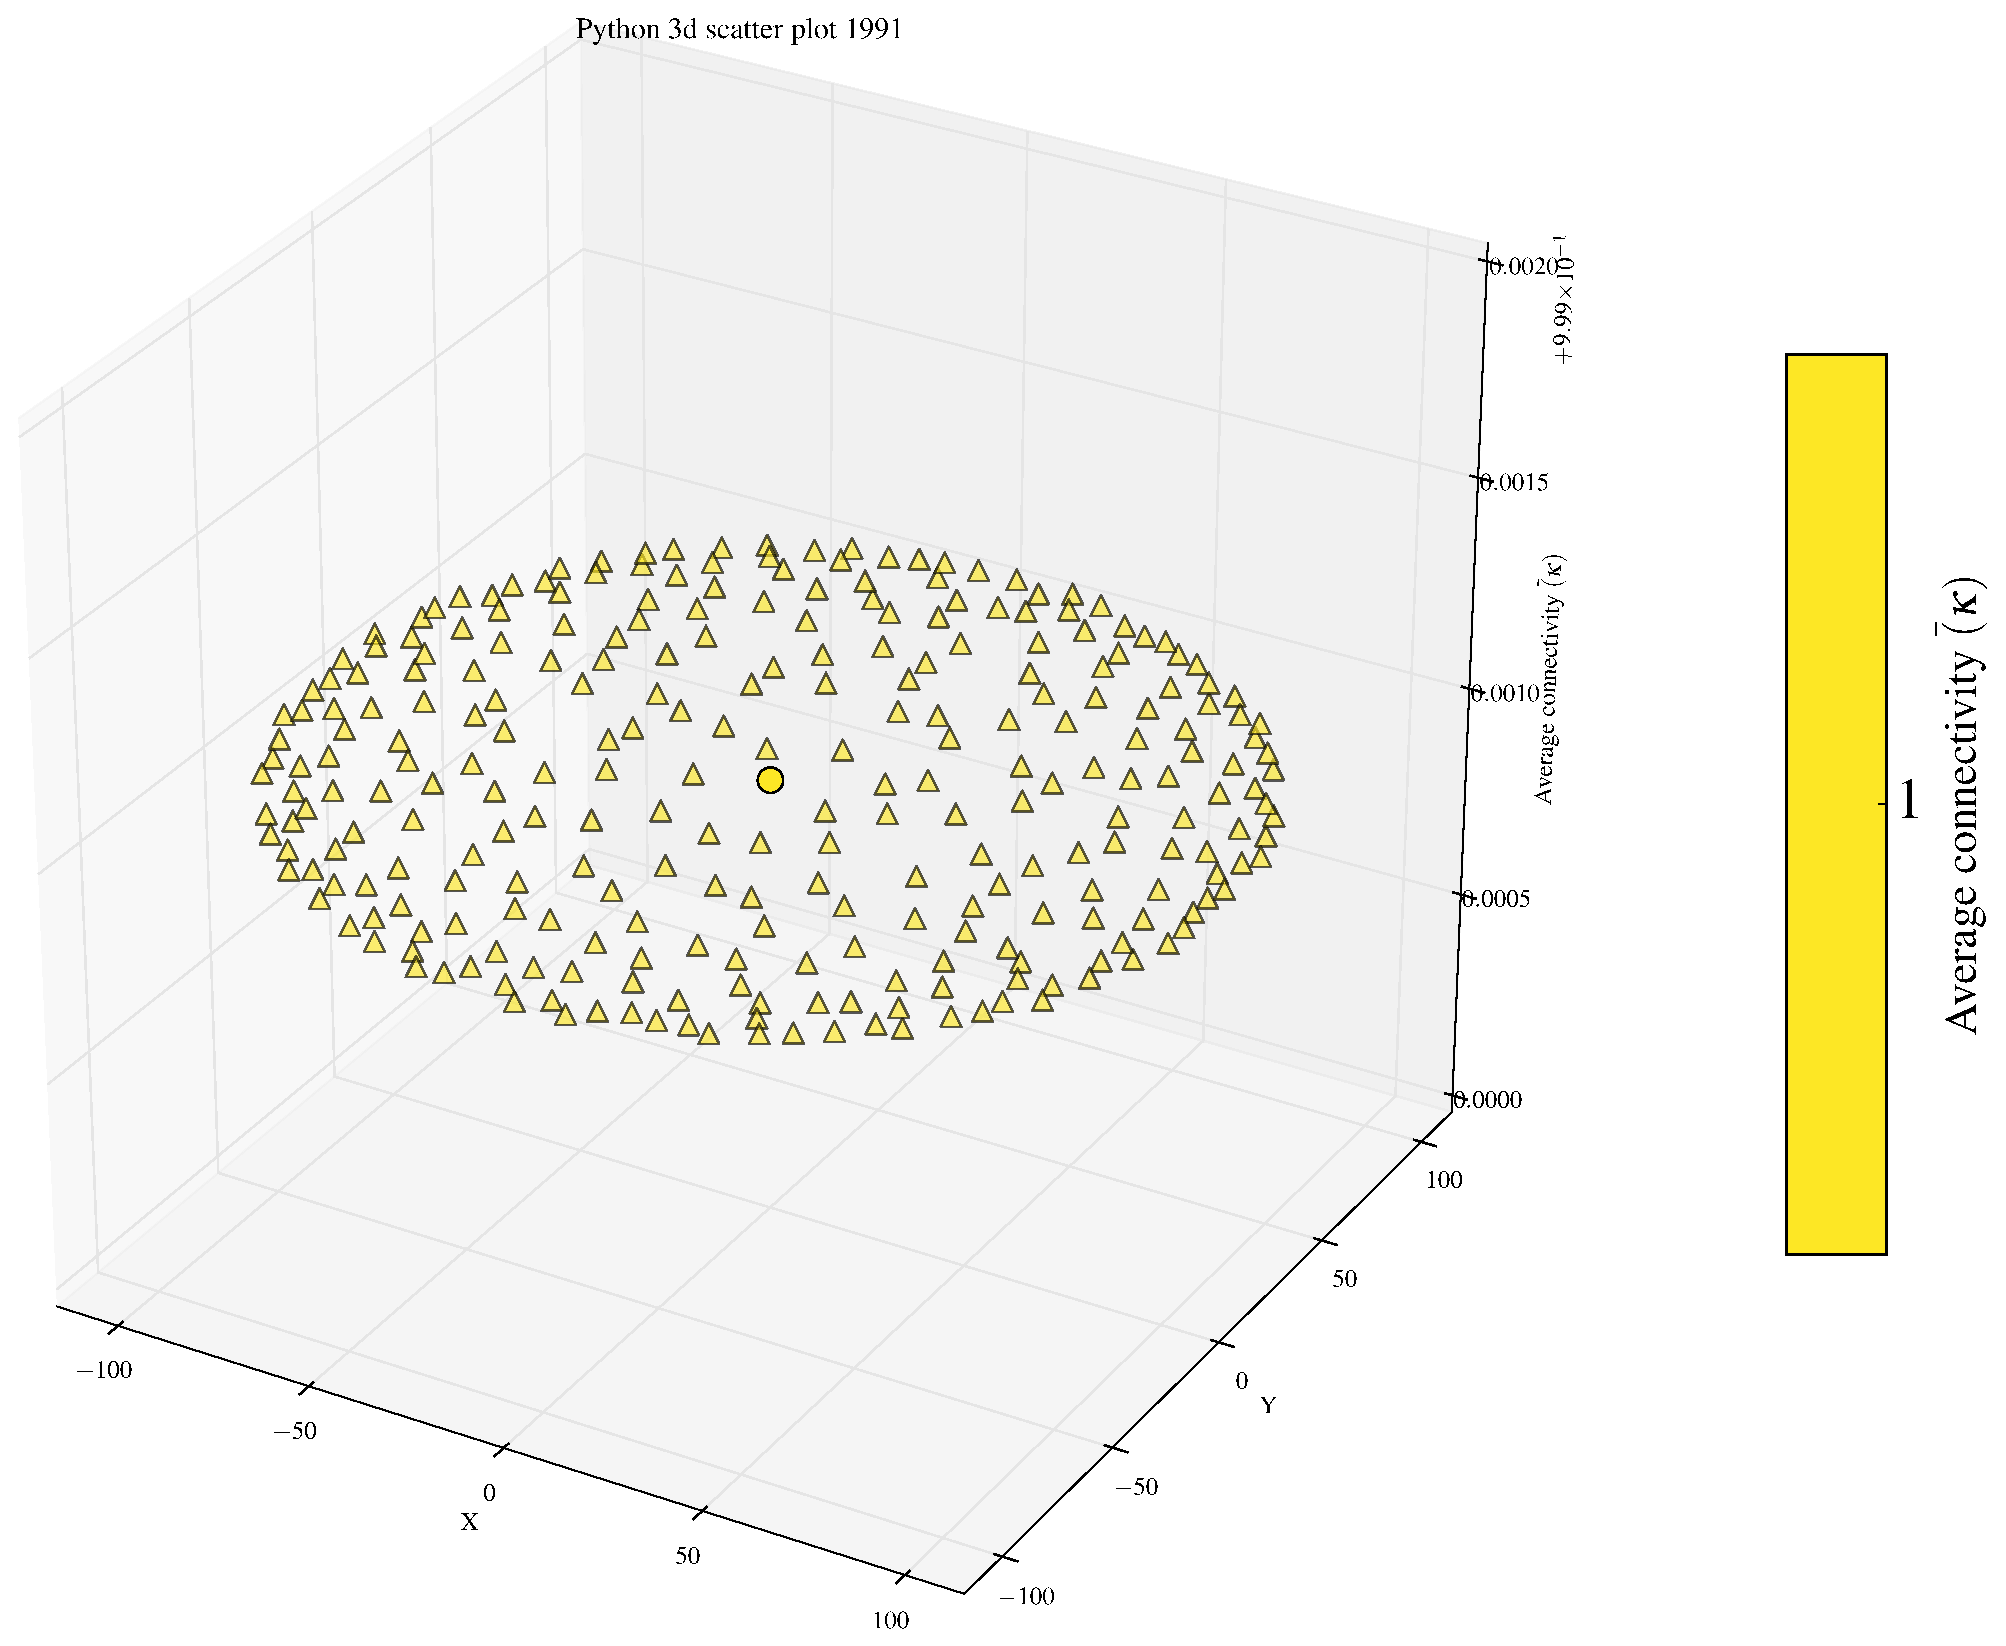
\includegraphics[scale=0.25]{img/3d_scatter_python_1991}
\end{center}

\end{frame}


\begin{frame}
\frametitle{Graphical Representation of the Structural Cohesion Analysis}

\begin{center}
\textbf{Python Cooperation Network 1999 (9 developers)}
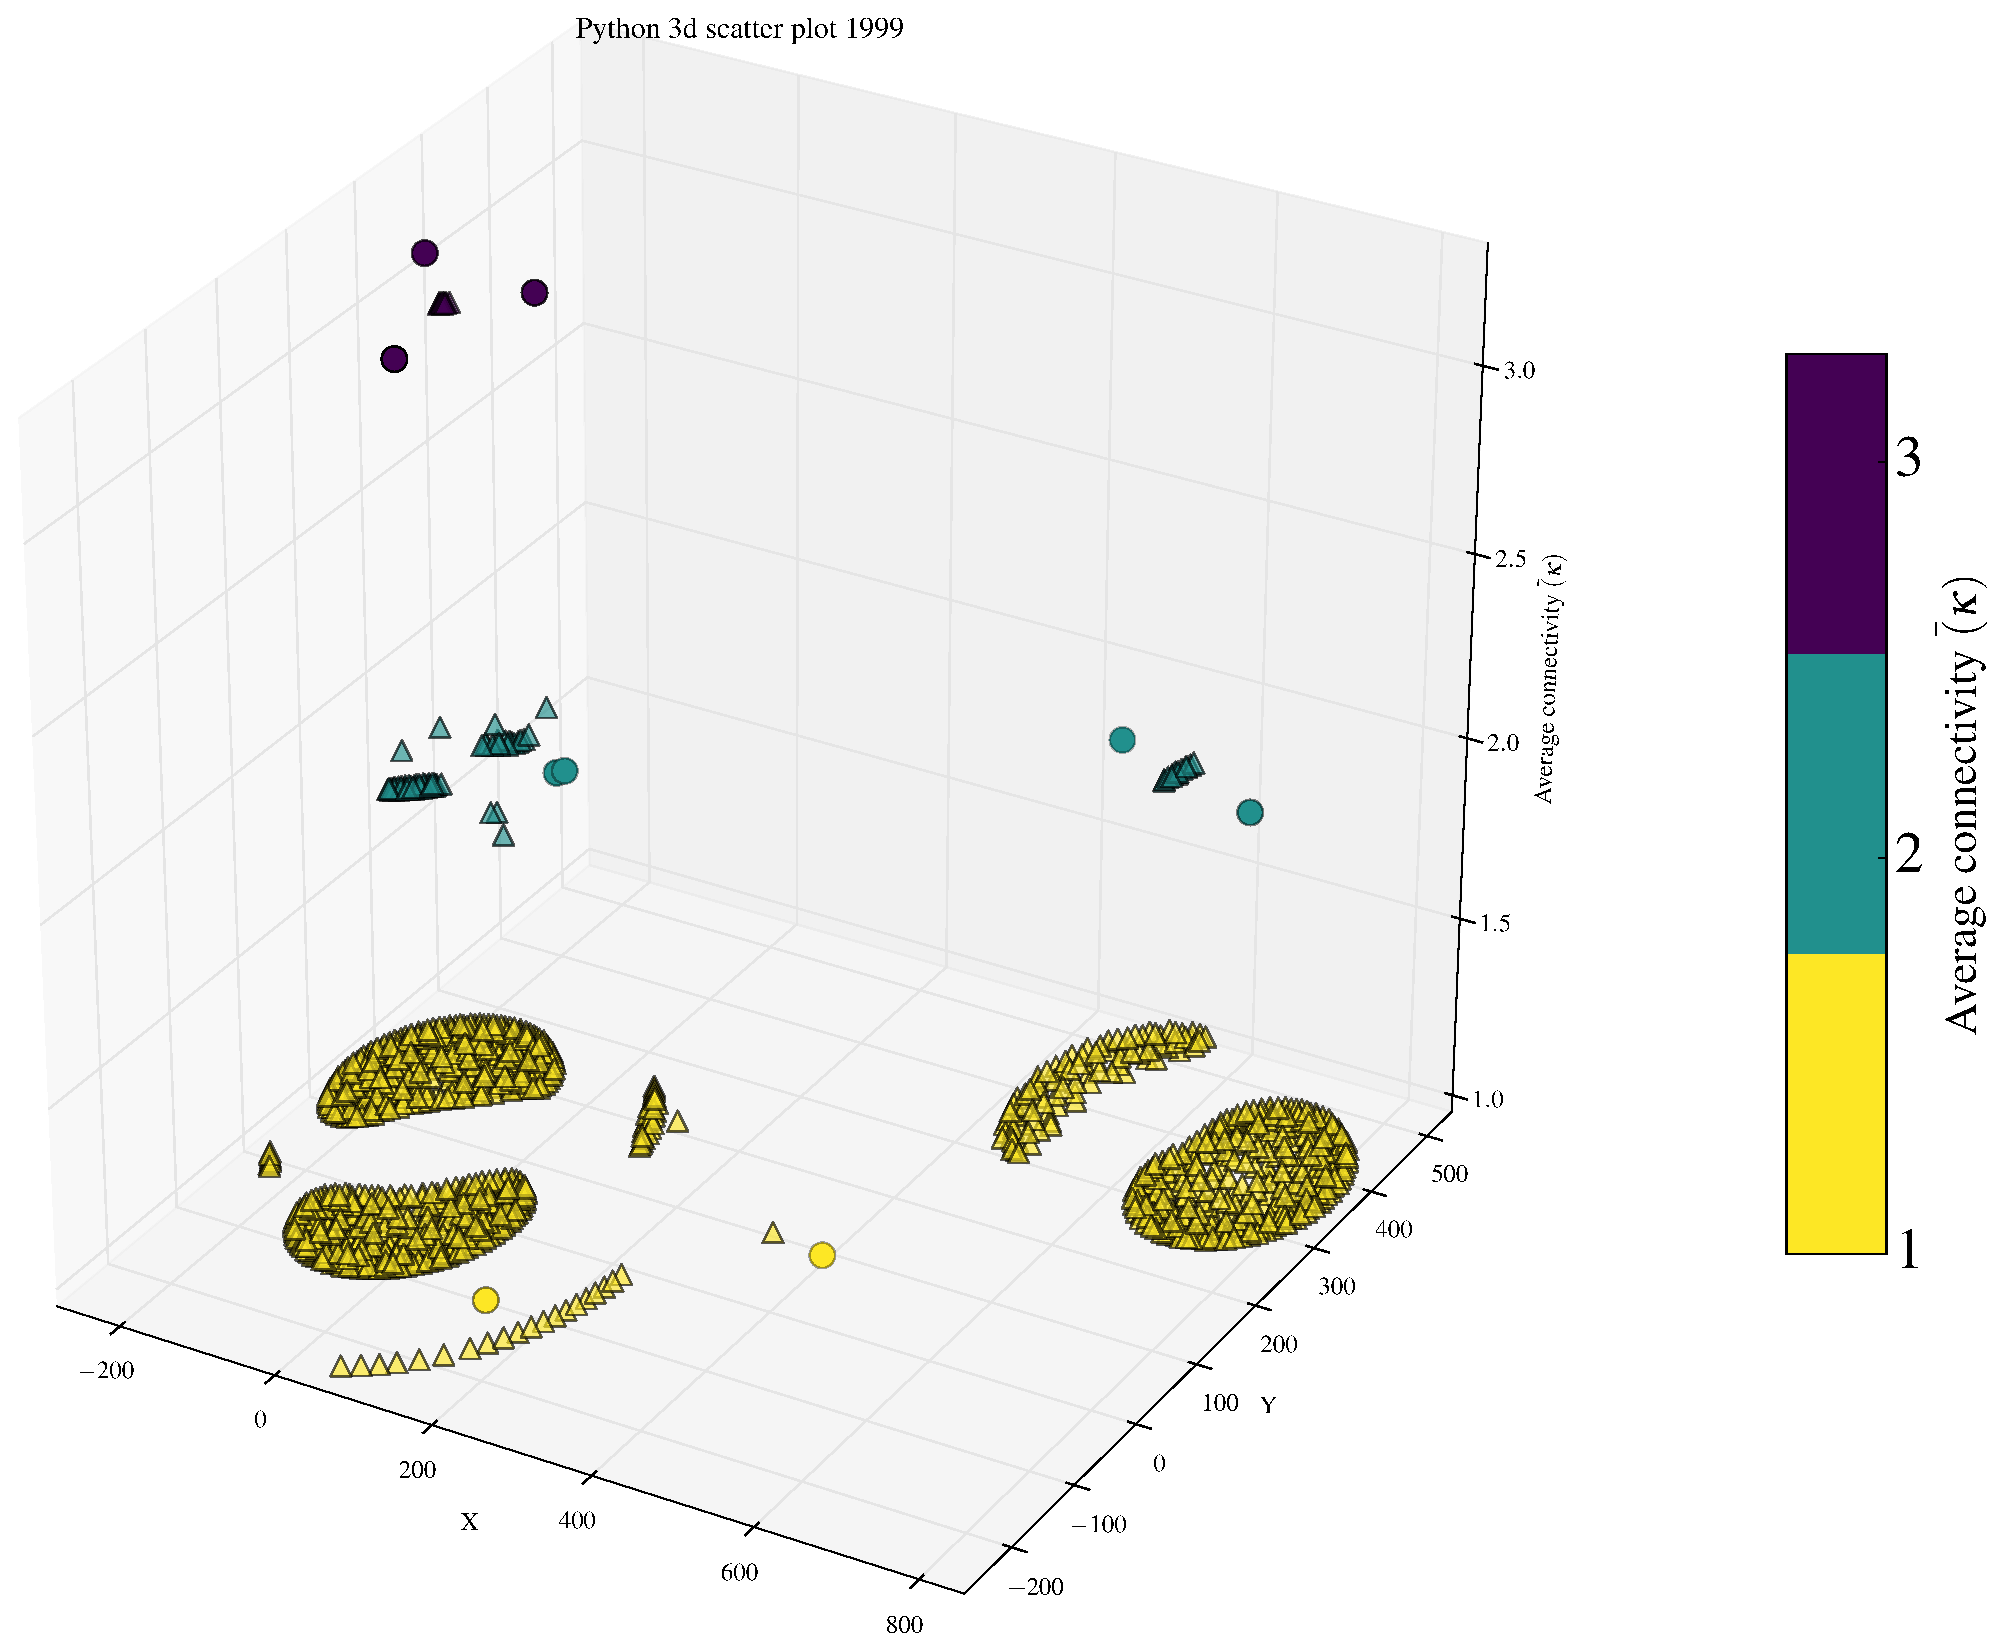
\includegraphics[scale=0.25]{img/3d_scatter_python_1999}
\end{center}

\end{frame}

\begin{frame}
\frametitle{Graphical Representation of the Structural Cohesion Analysis}

\begin{center}
\textbf{Python Cooperation Network 2000 (31 developers)}
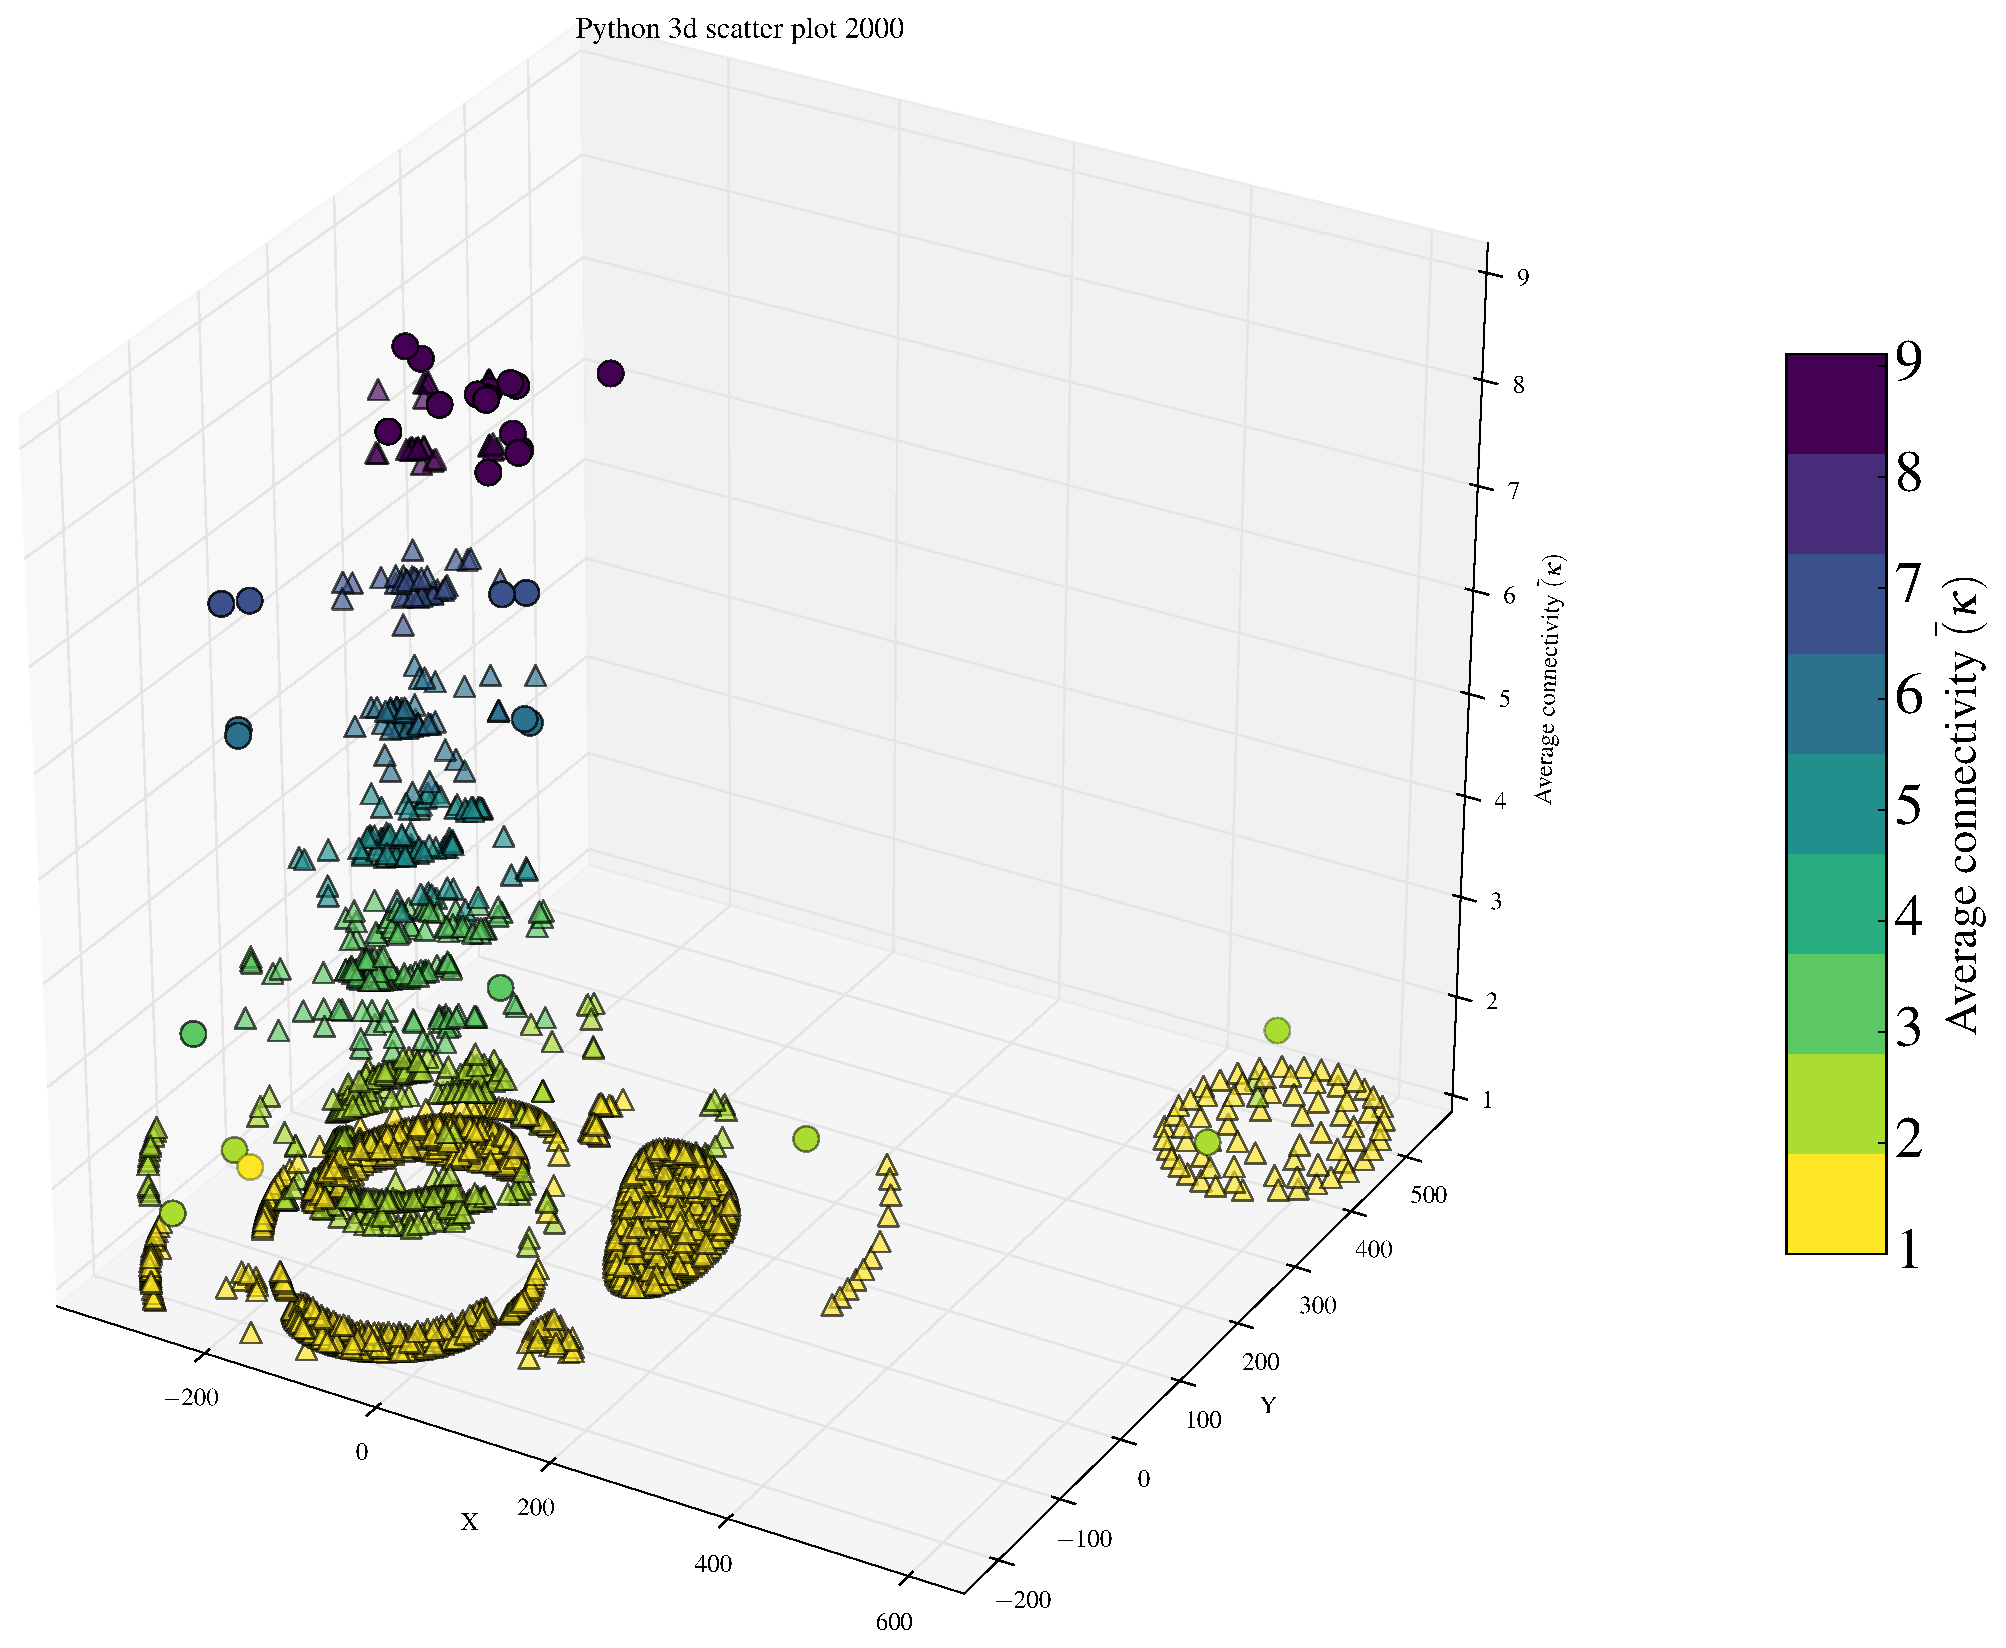
\includegraphics[scale=0.25]{img/3d_scatter_python_2000}
\end{center}

\end{frame}

\begin{frame}
\frametitle{Graphical Representation of the Structural Cohesion Analysis}

\begin{center}
\textbf{Python Cooperation Network 2001 (33 developers)}
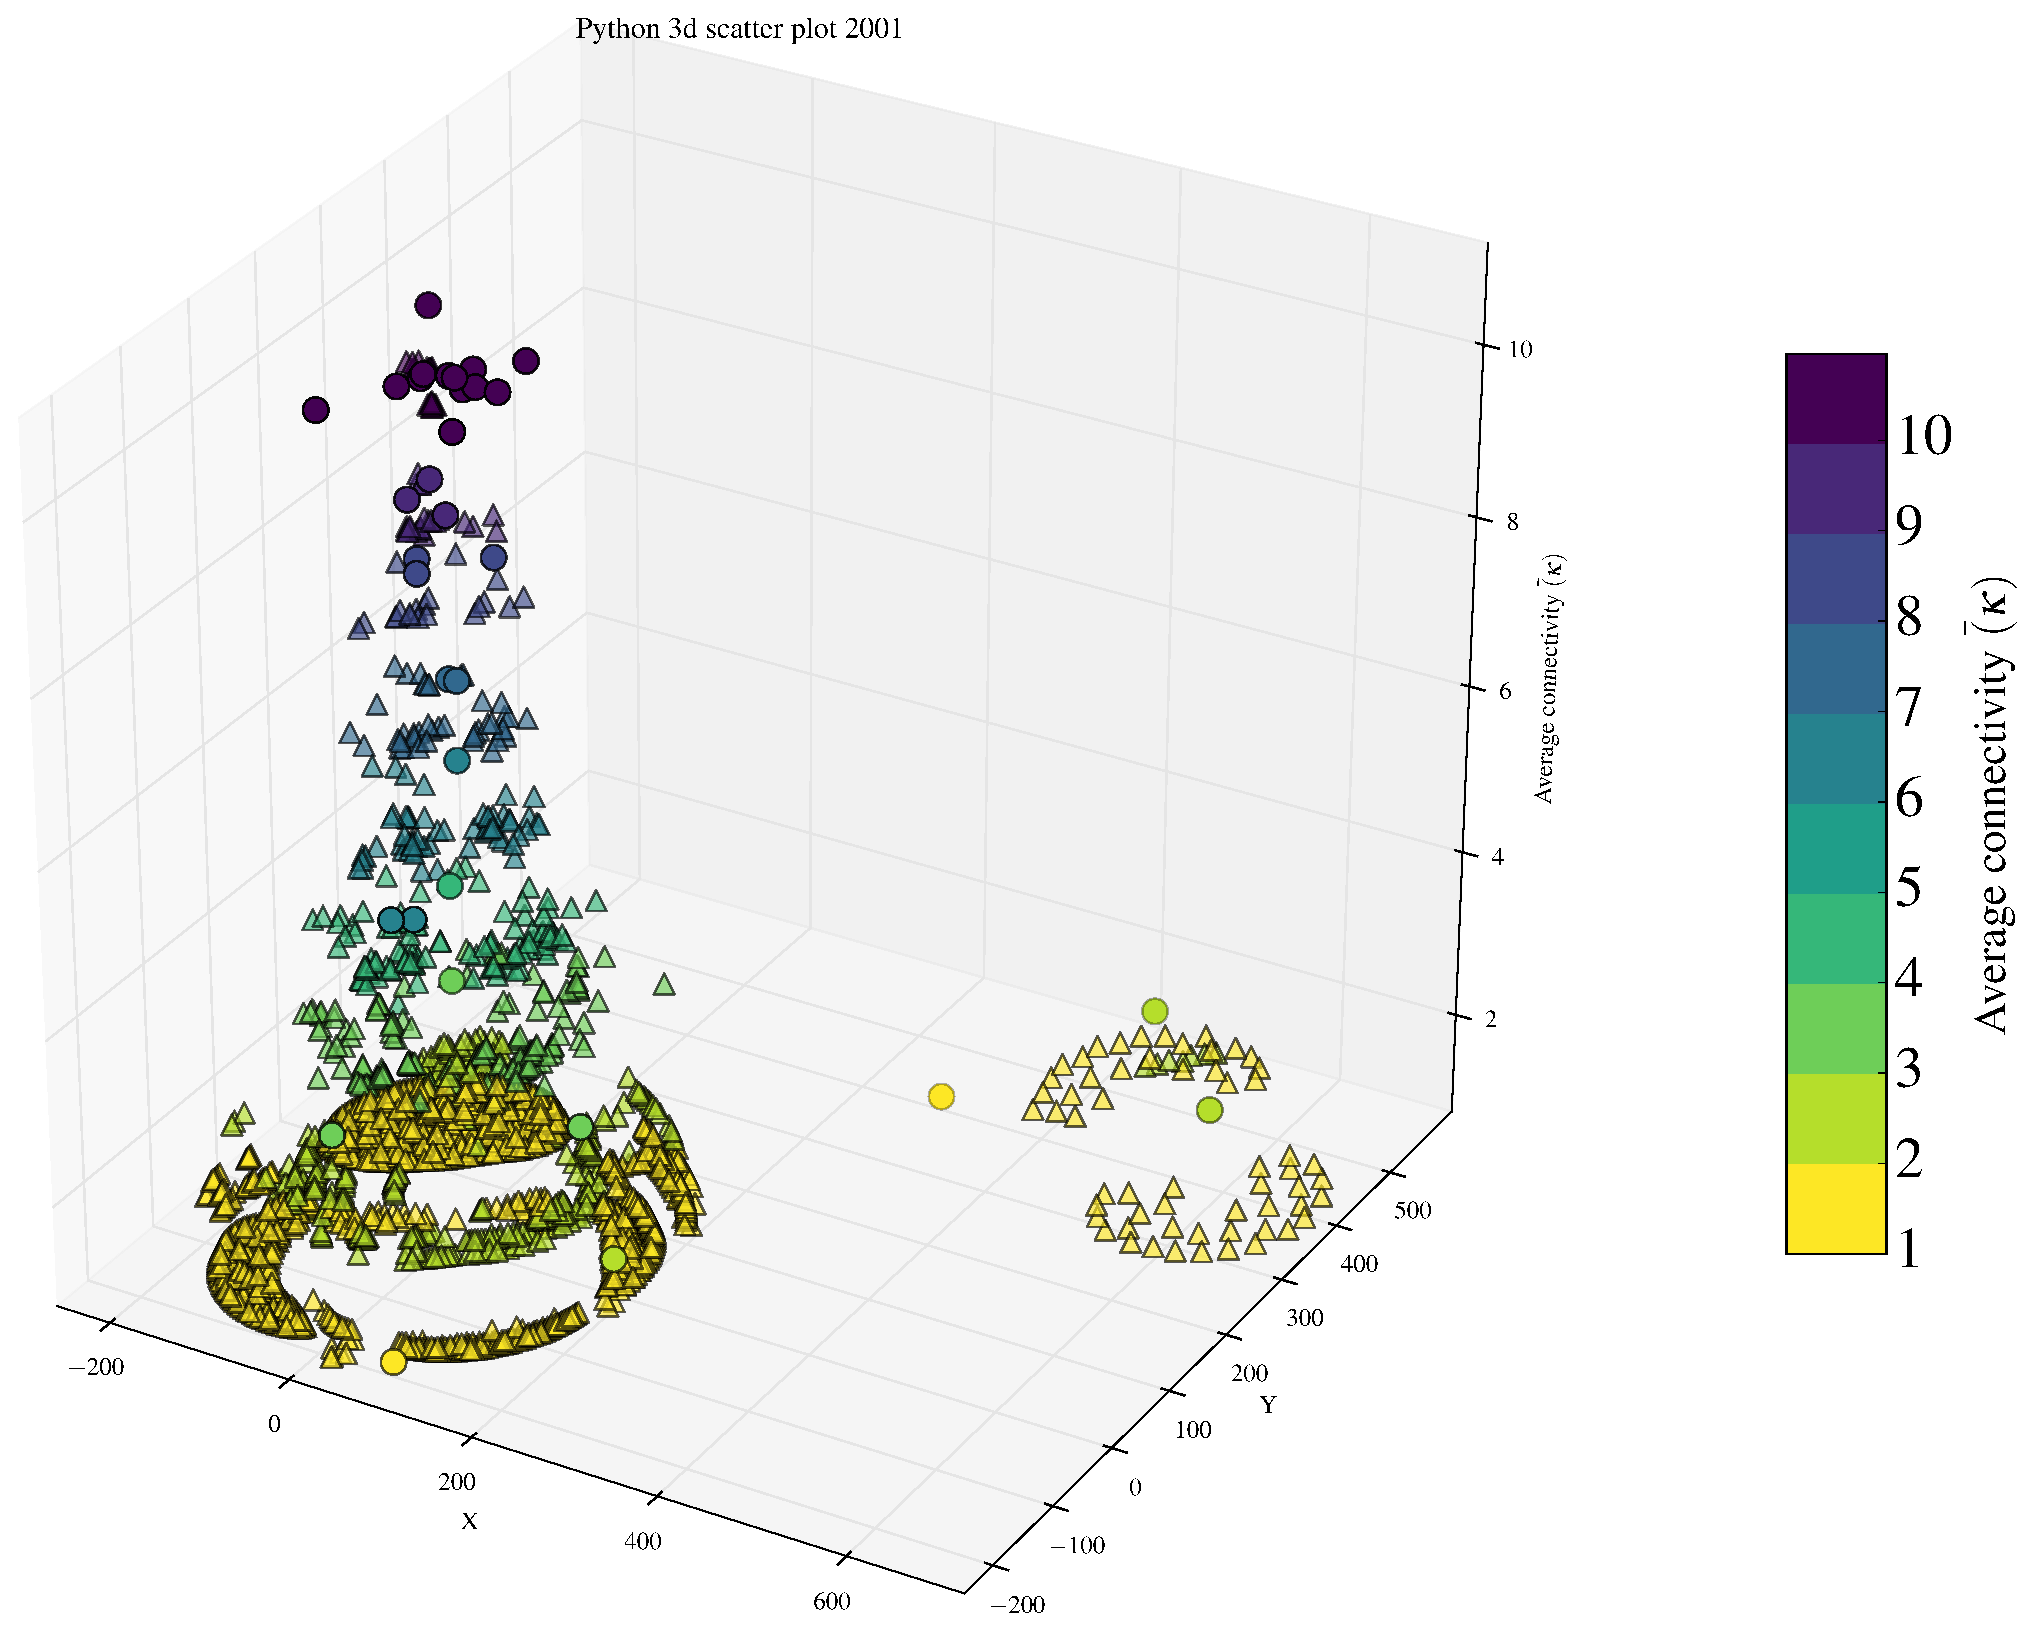
\includegraphics[scale=0.25]{img/3d_scatter_python_2001}
\end{center}

\end{frame}


\begin{frame}
\frametitle{Graphical Representation of the Structural Cohesion Analysis}

\begin{center}
\textbf{Python Cooperation Network 2002 (38 developers)}
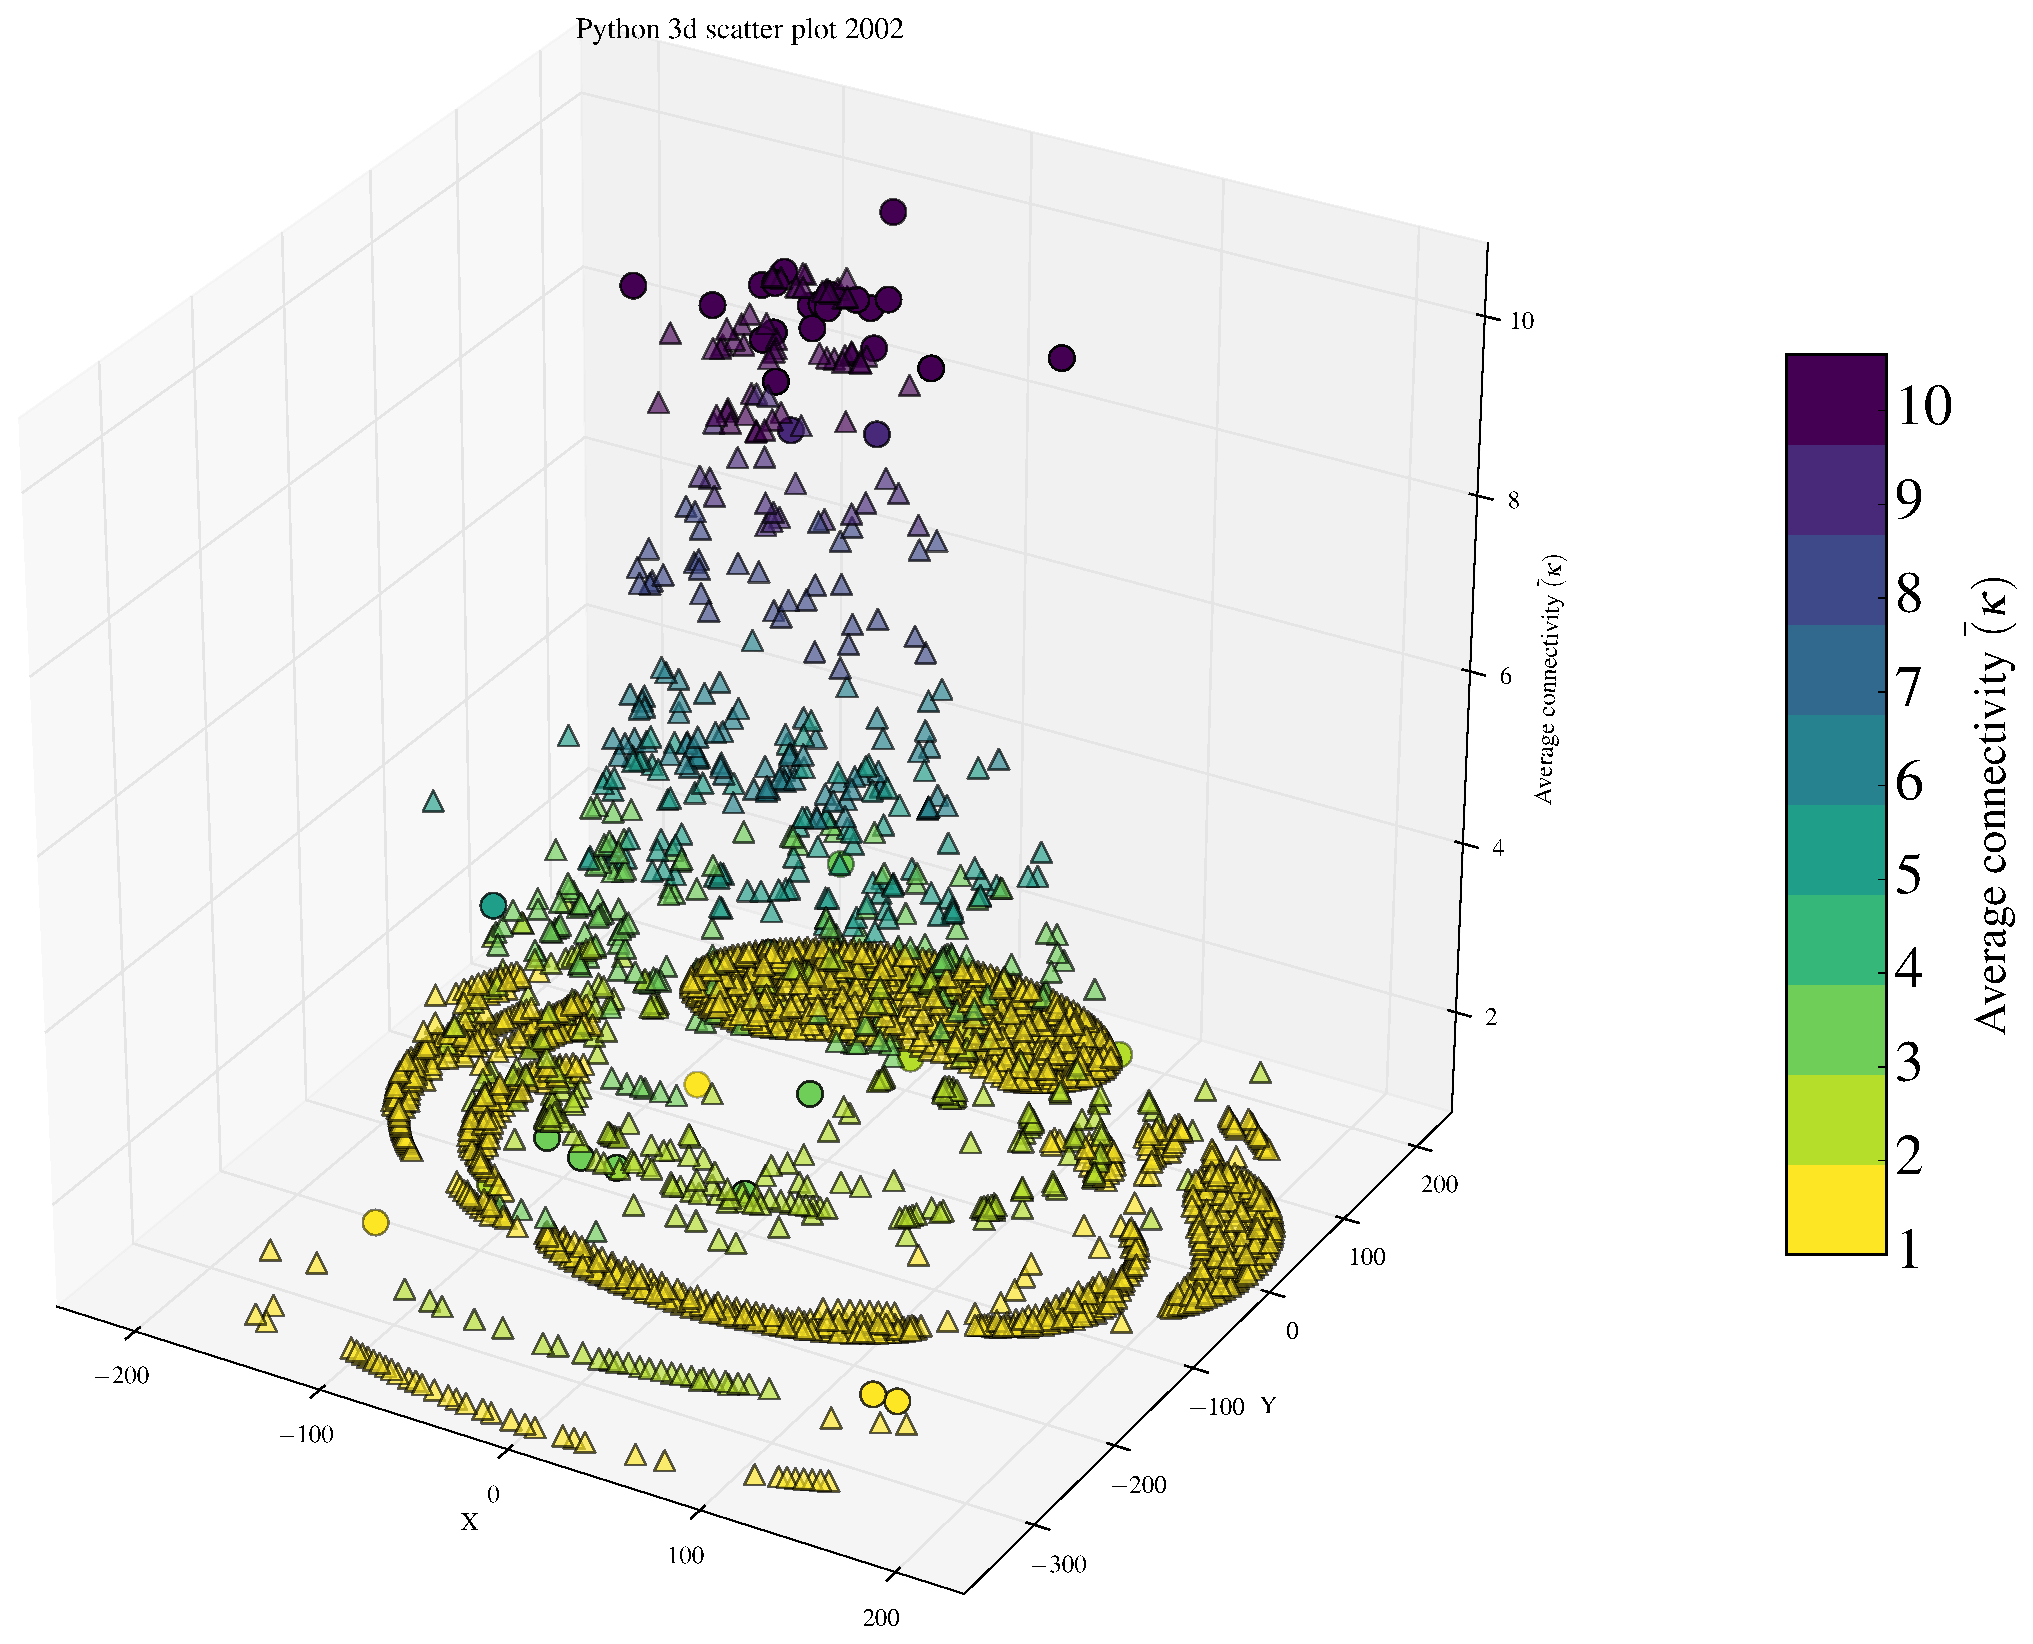
\includegraphics[scale=0.25]{img/3d_scatter_python_2002}
\end{center}

\end{frame}

\begin{frame}
\frametitle{Graphical Representation of the Structural Cohesion Analysis}

\begin{center}
\textbf{Python Cooperation Network 2003 (42 developers)}
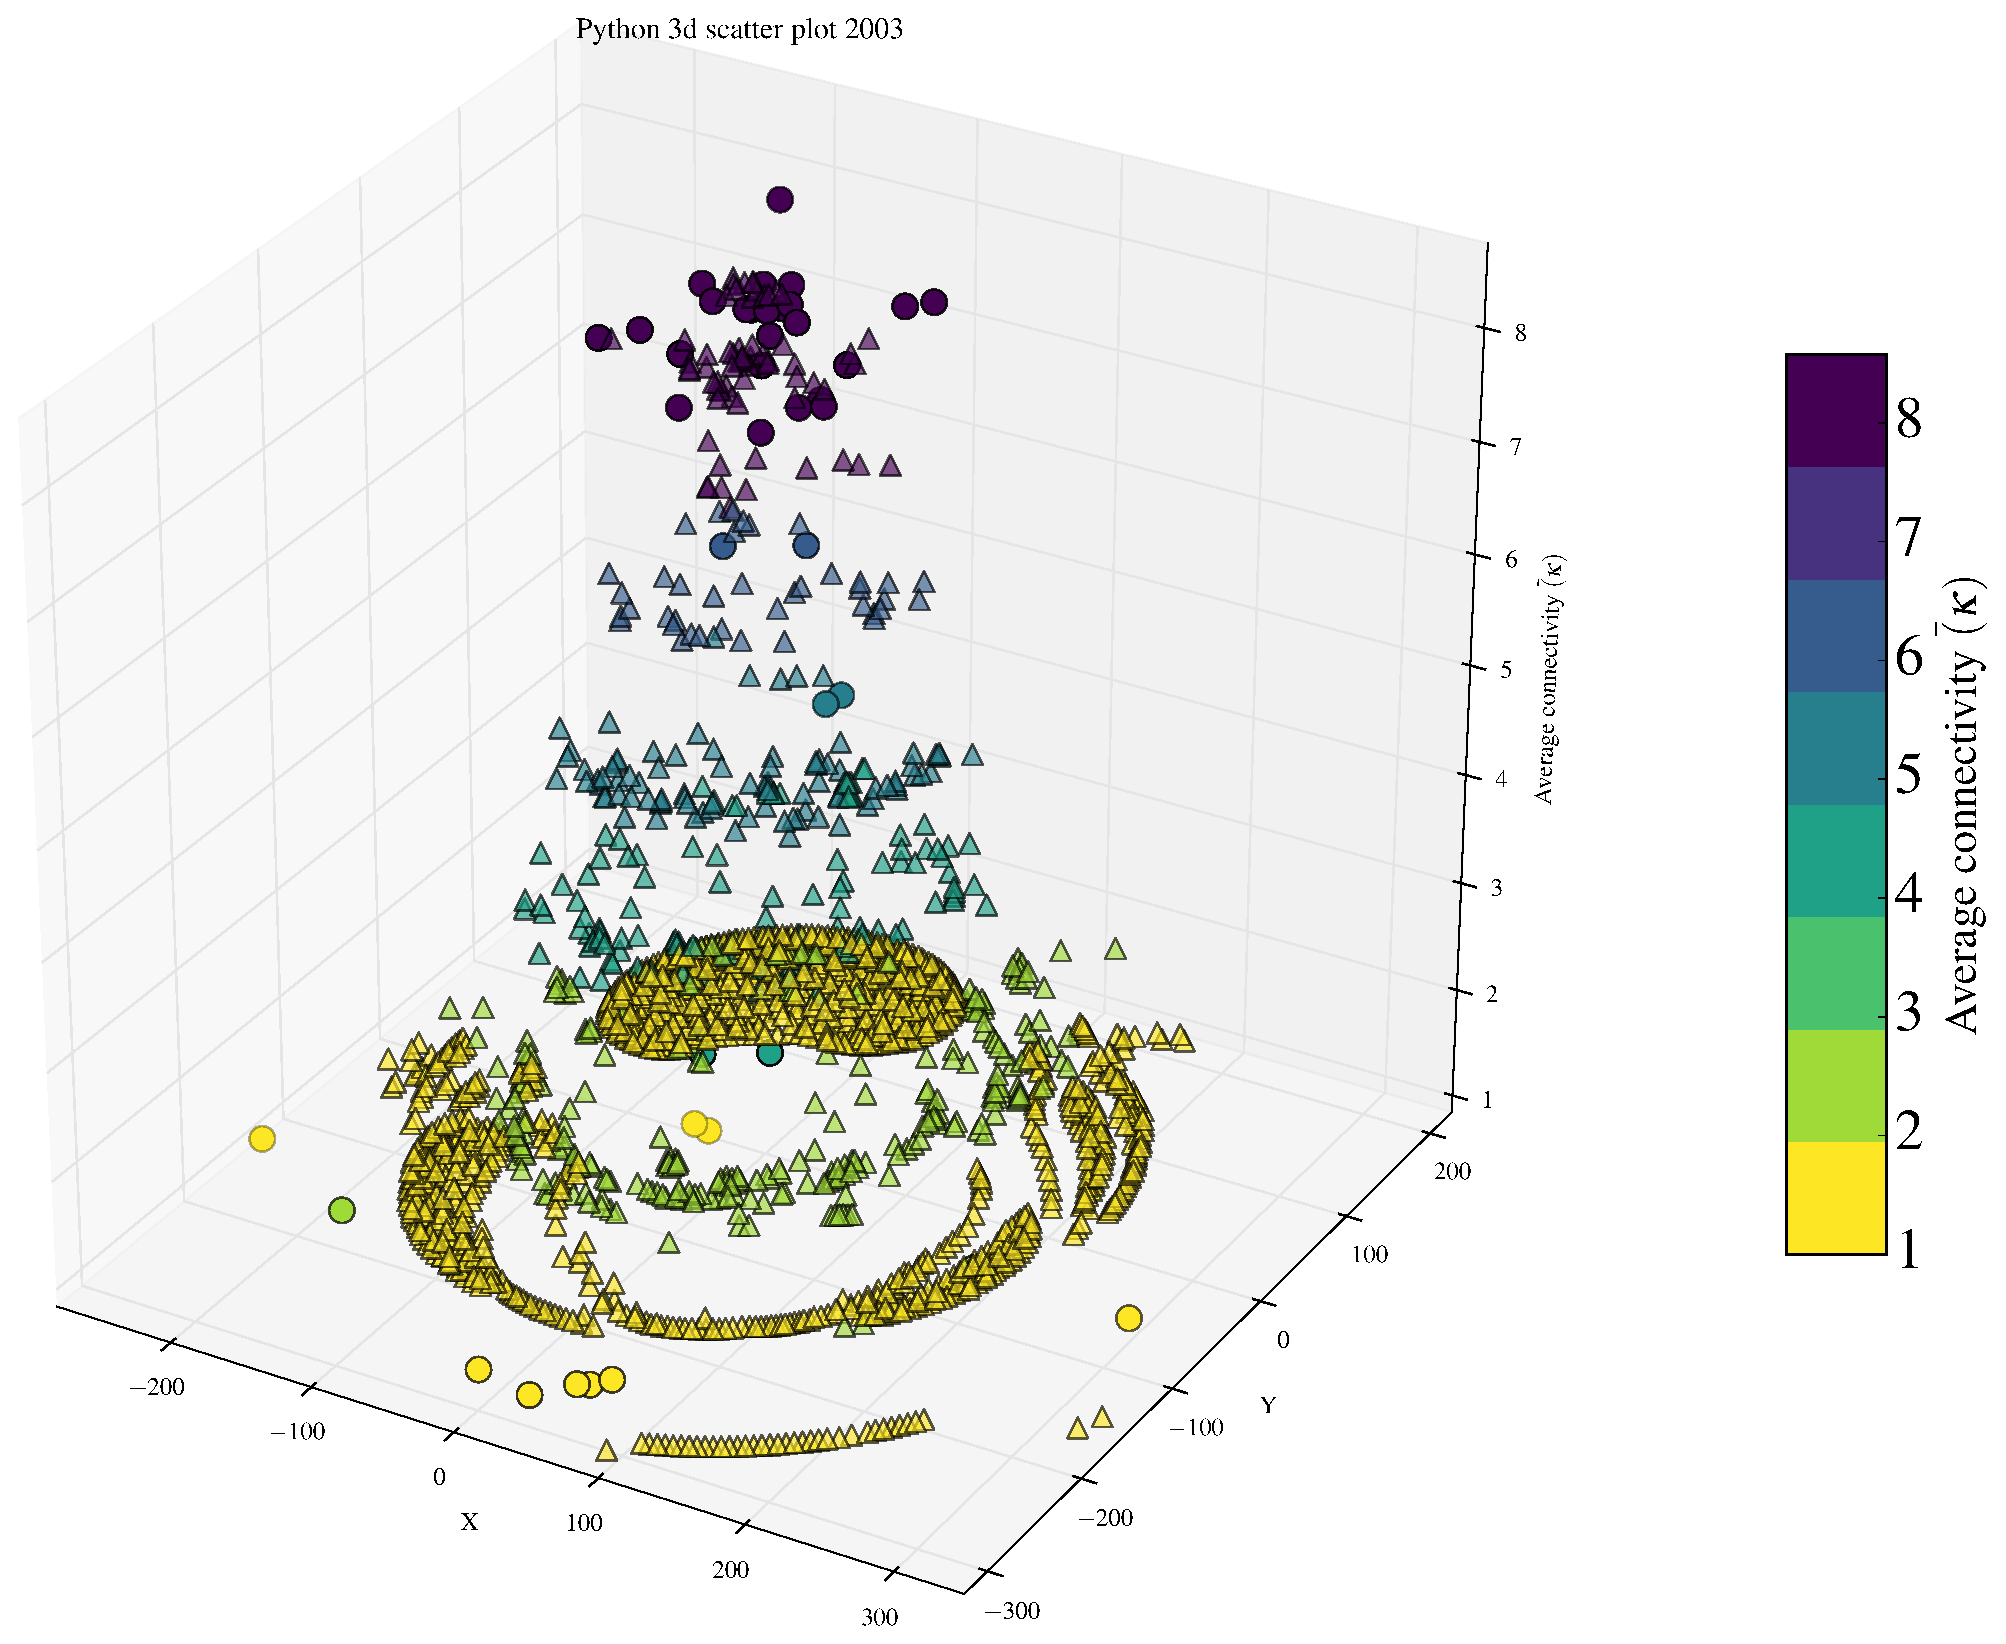
\includegraphics[scale=0.25]{img/3d_scatter_python_2003}
\end{center}

\end{frame}

\begin{frame}
\frametitle{Graphical Representation of the Structural Cohesion Analysis}

\begin{center}
\textbf{Python Cooperation Network 2004 (49 developers)}
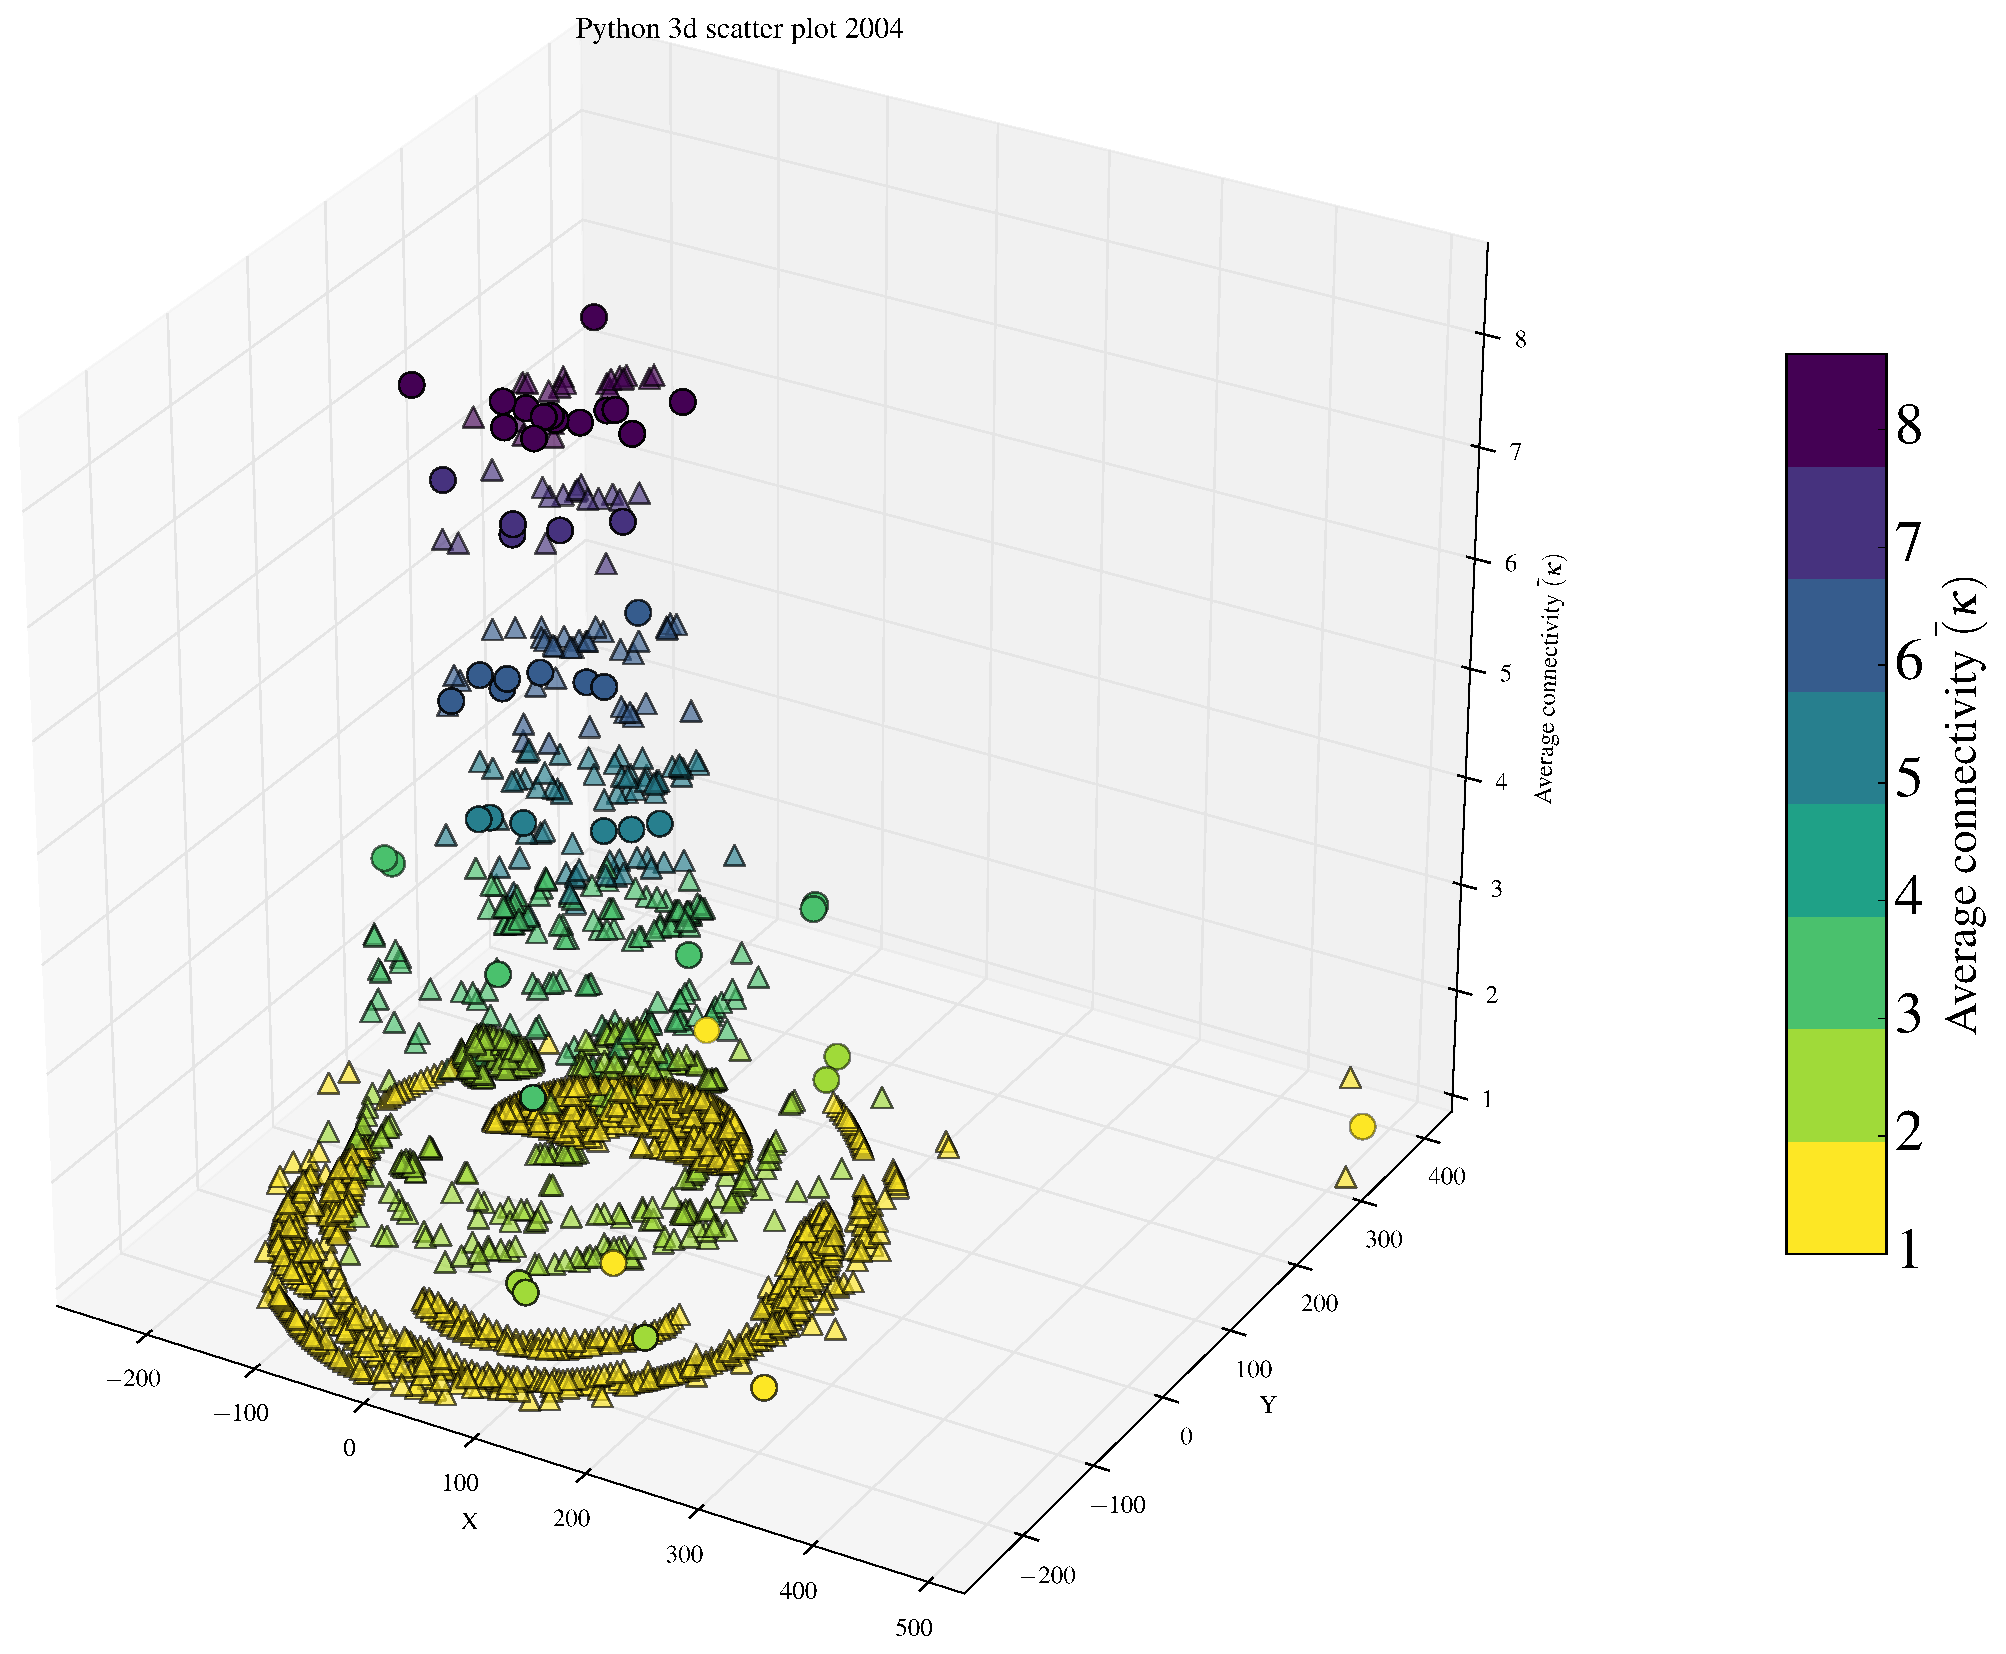
\includegraphics[scale=0.25]{img/3d_scatter_python_2004}
\end{center}

\end{frame}

\begin{frame}
\frametitle{Graphical Representation of the Structural Cohesion Analysis}

\begin{center}
\textbf{Python Cooperation Network 2005 (44 developers)}
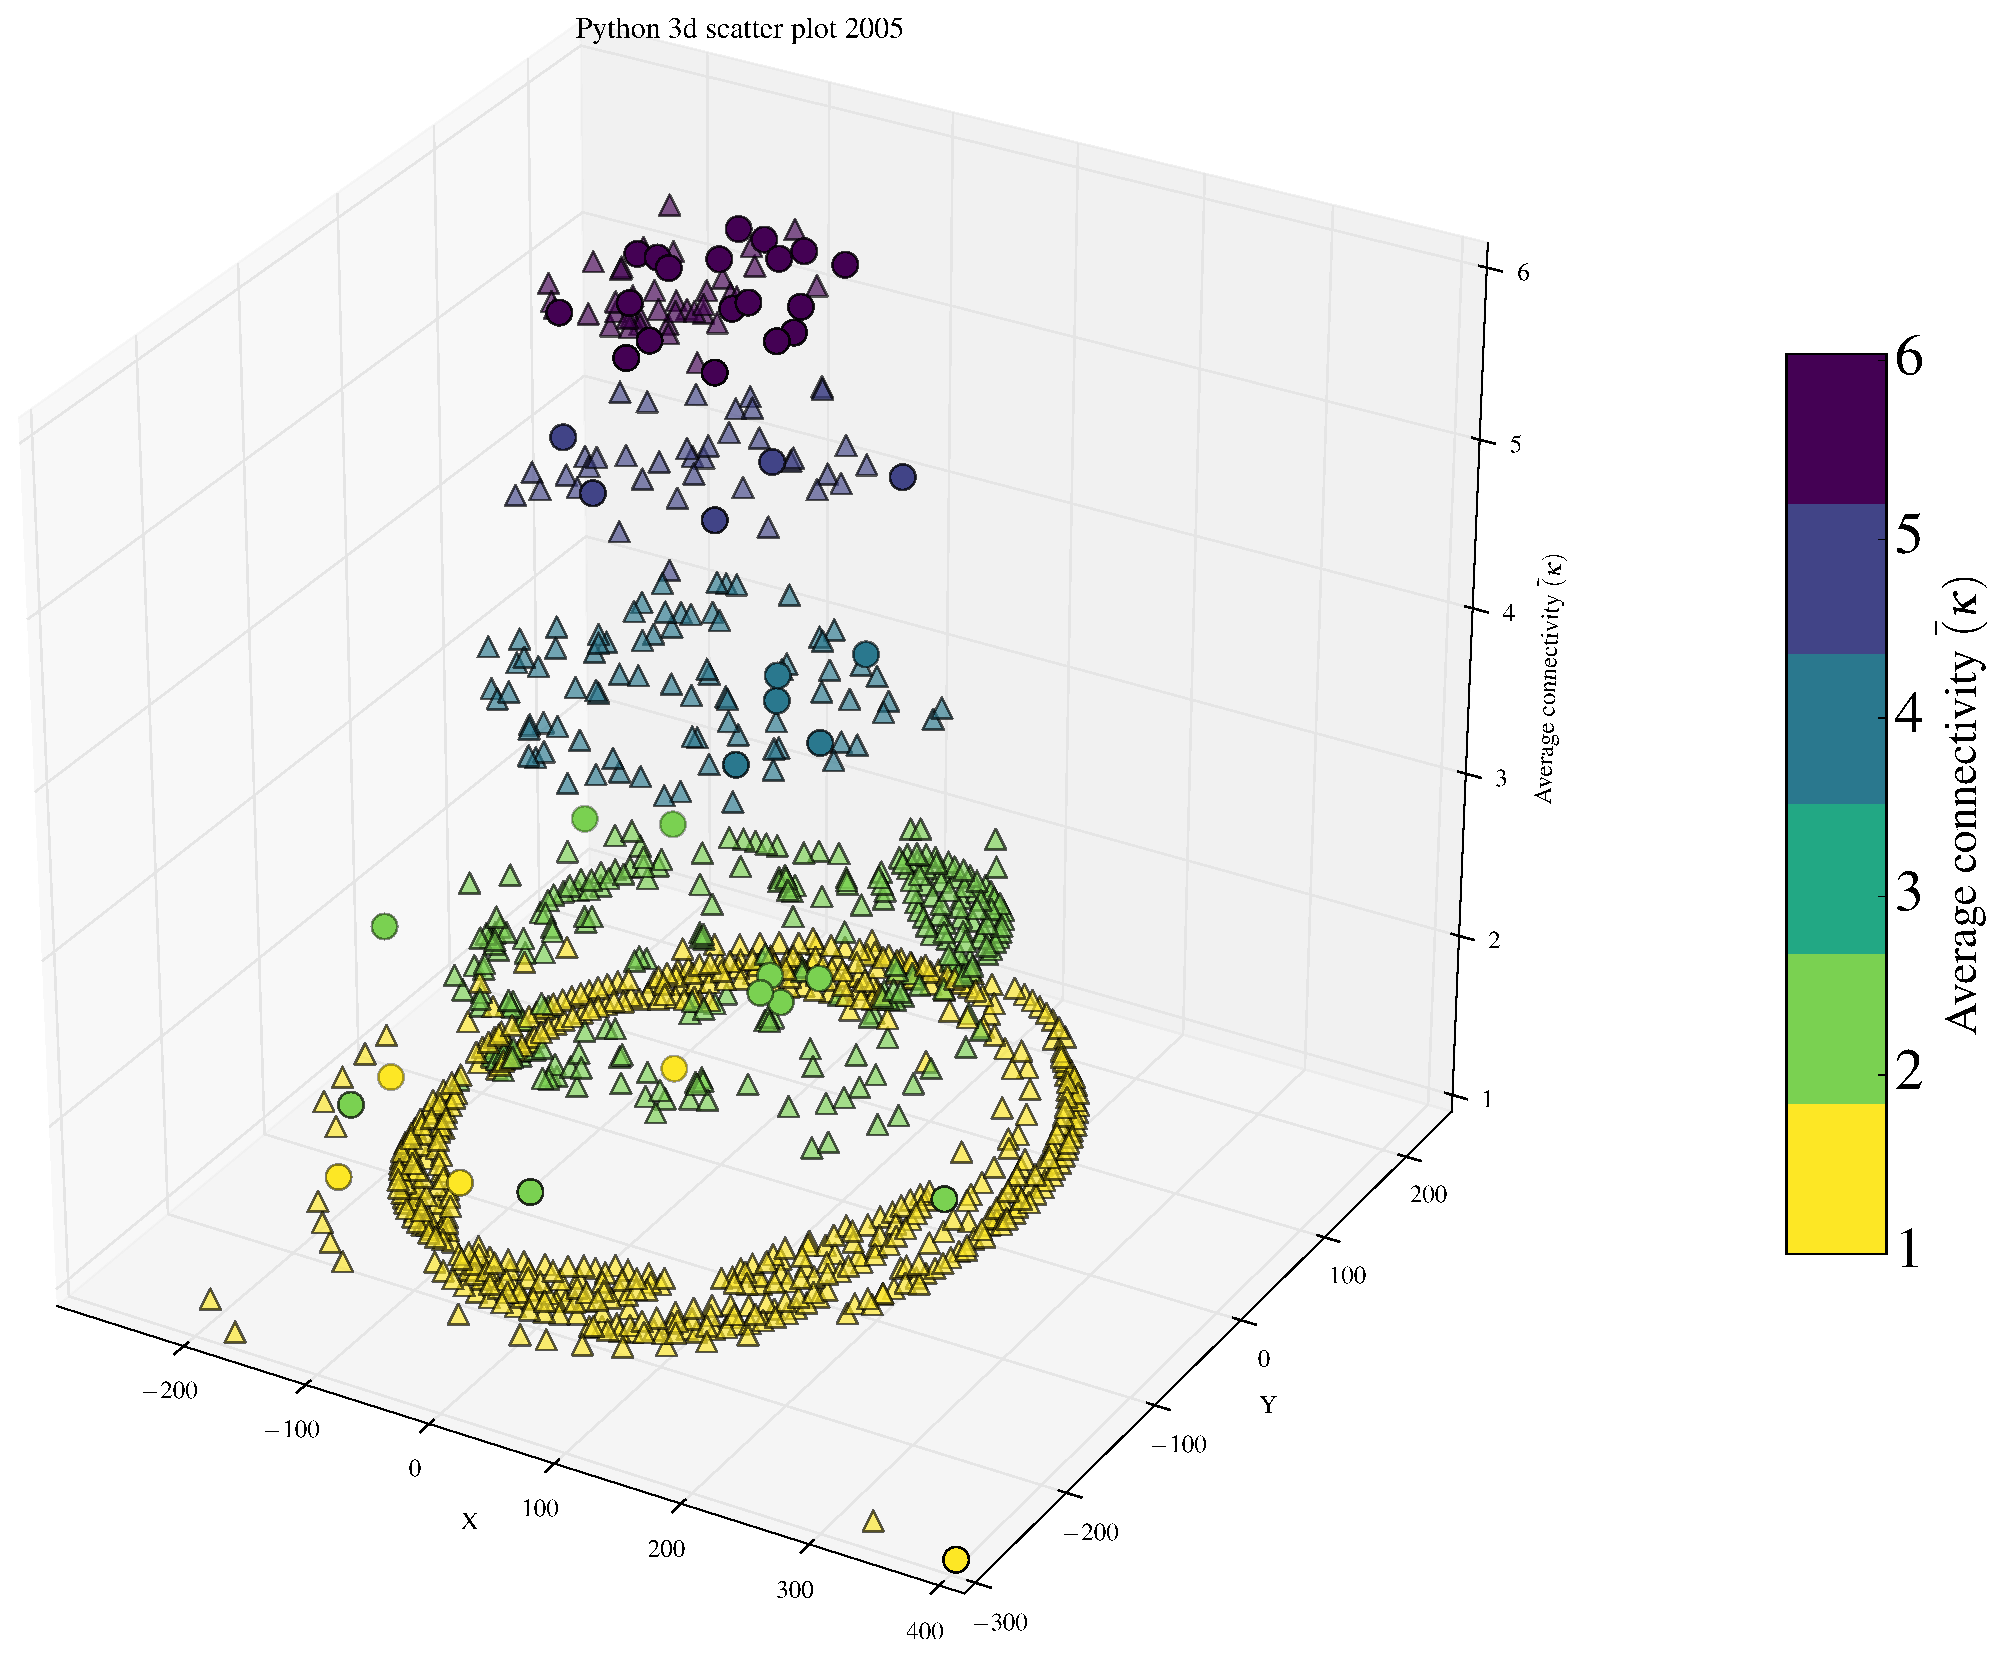
\includegraphics[scale=0.25]{img/3d_scatter_python_2005}
\end{center}

\end{frame}

\begin{frame}
\frametitle{Graphical Representation of the Structural Cohesion Analysis}

\begin{center}
\textbf{Python Cooperation Network 2006 (52 developers)}
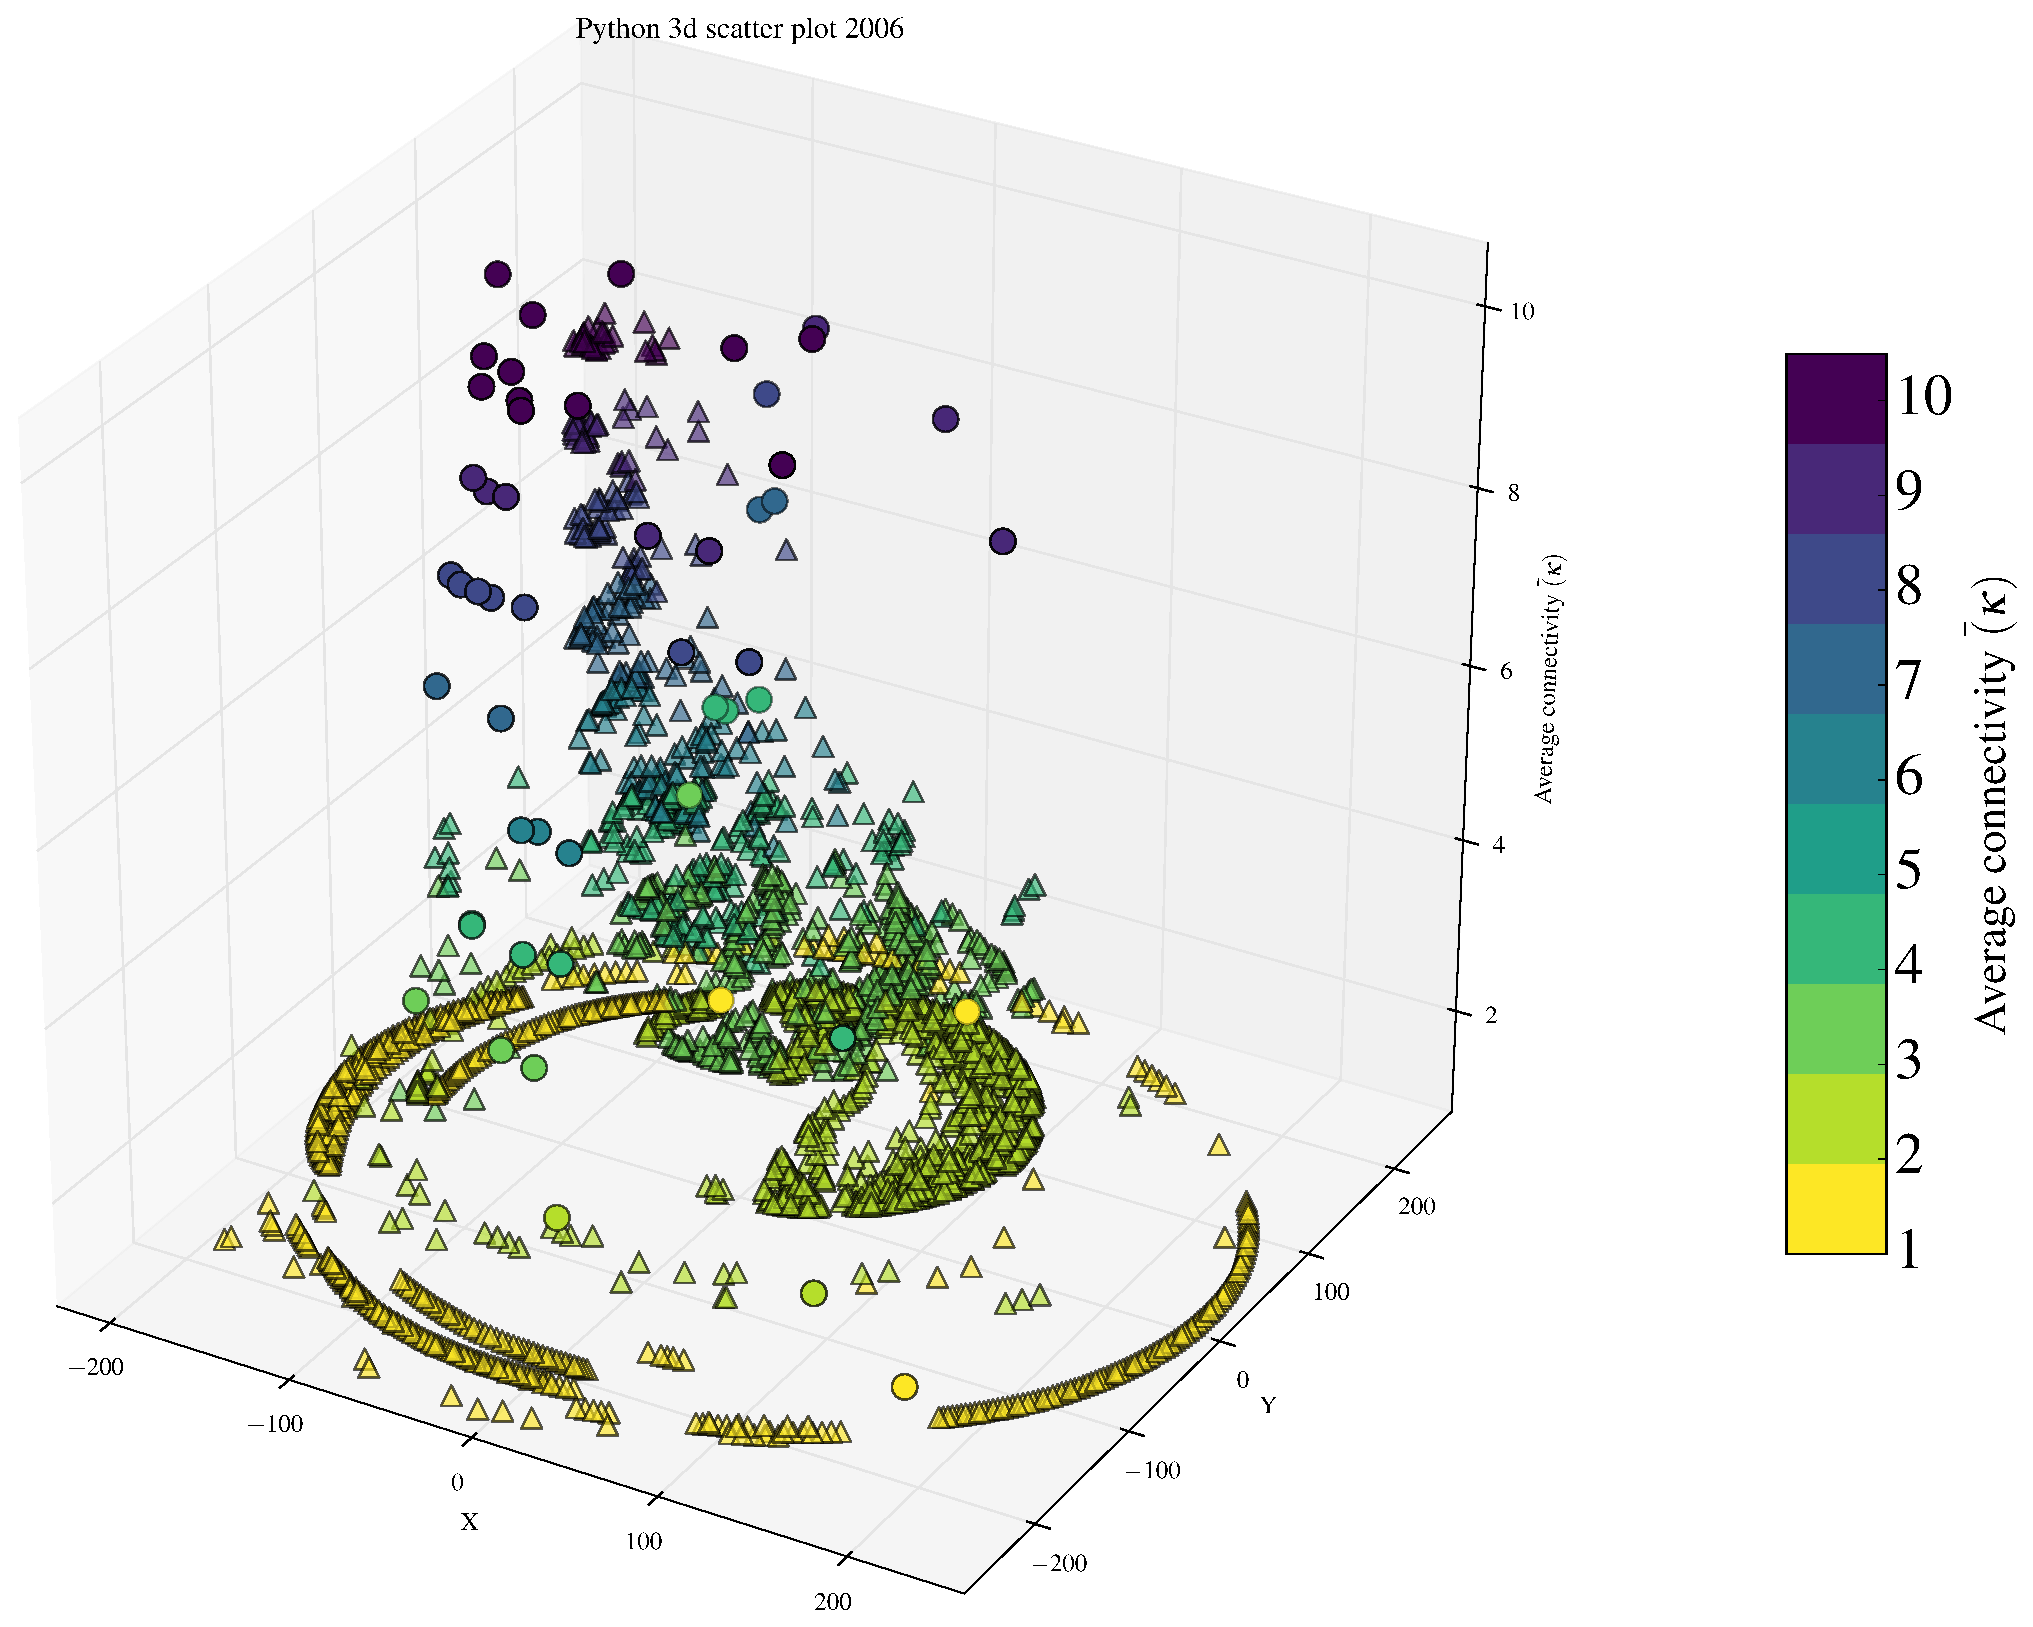
\includegraphics[scale=0.25]{img/3d_scatter_python_2006}
\end{center}

\end{frame}

\begin{frame}
\frametitle{Graphical Representation of the Structural Cohesion Analysis}

\begin{center}
\textbf{Python Cooperation Network 2007 (51 developers)}
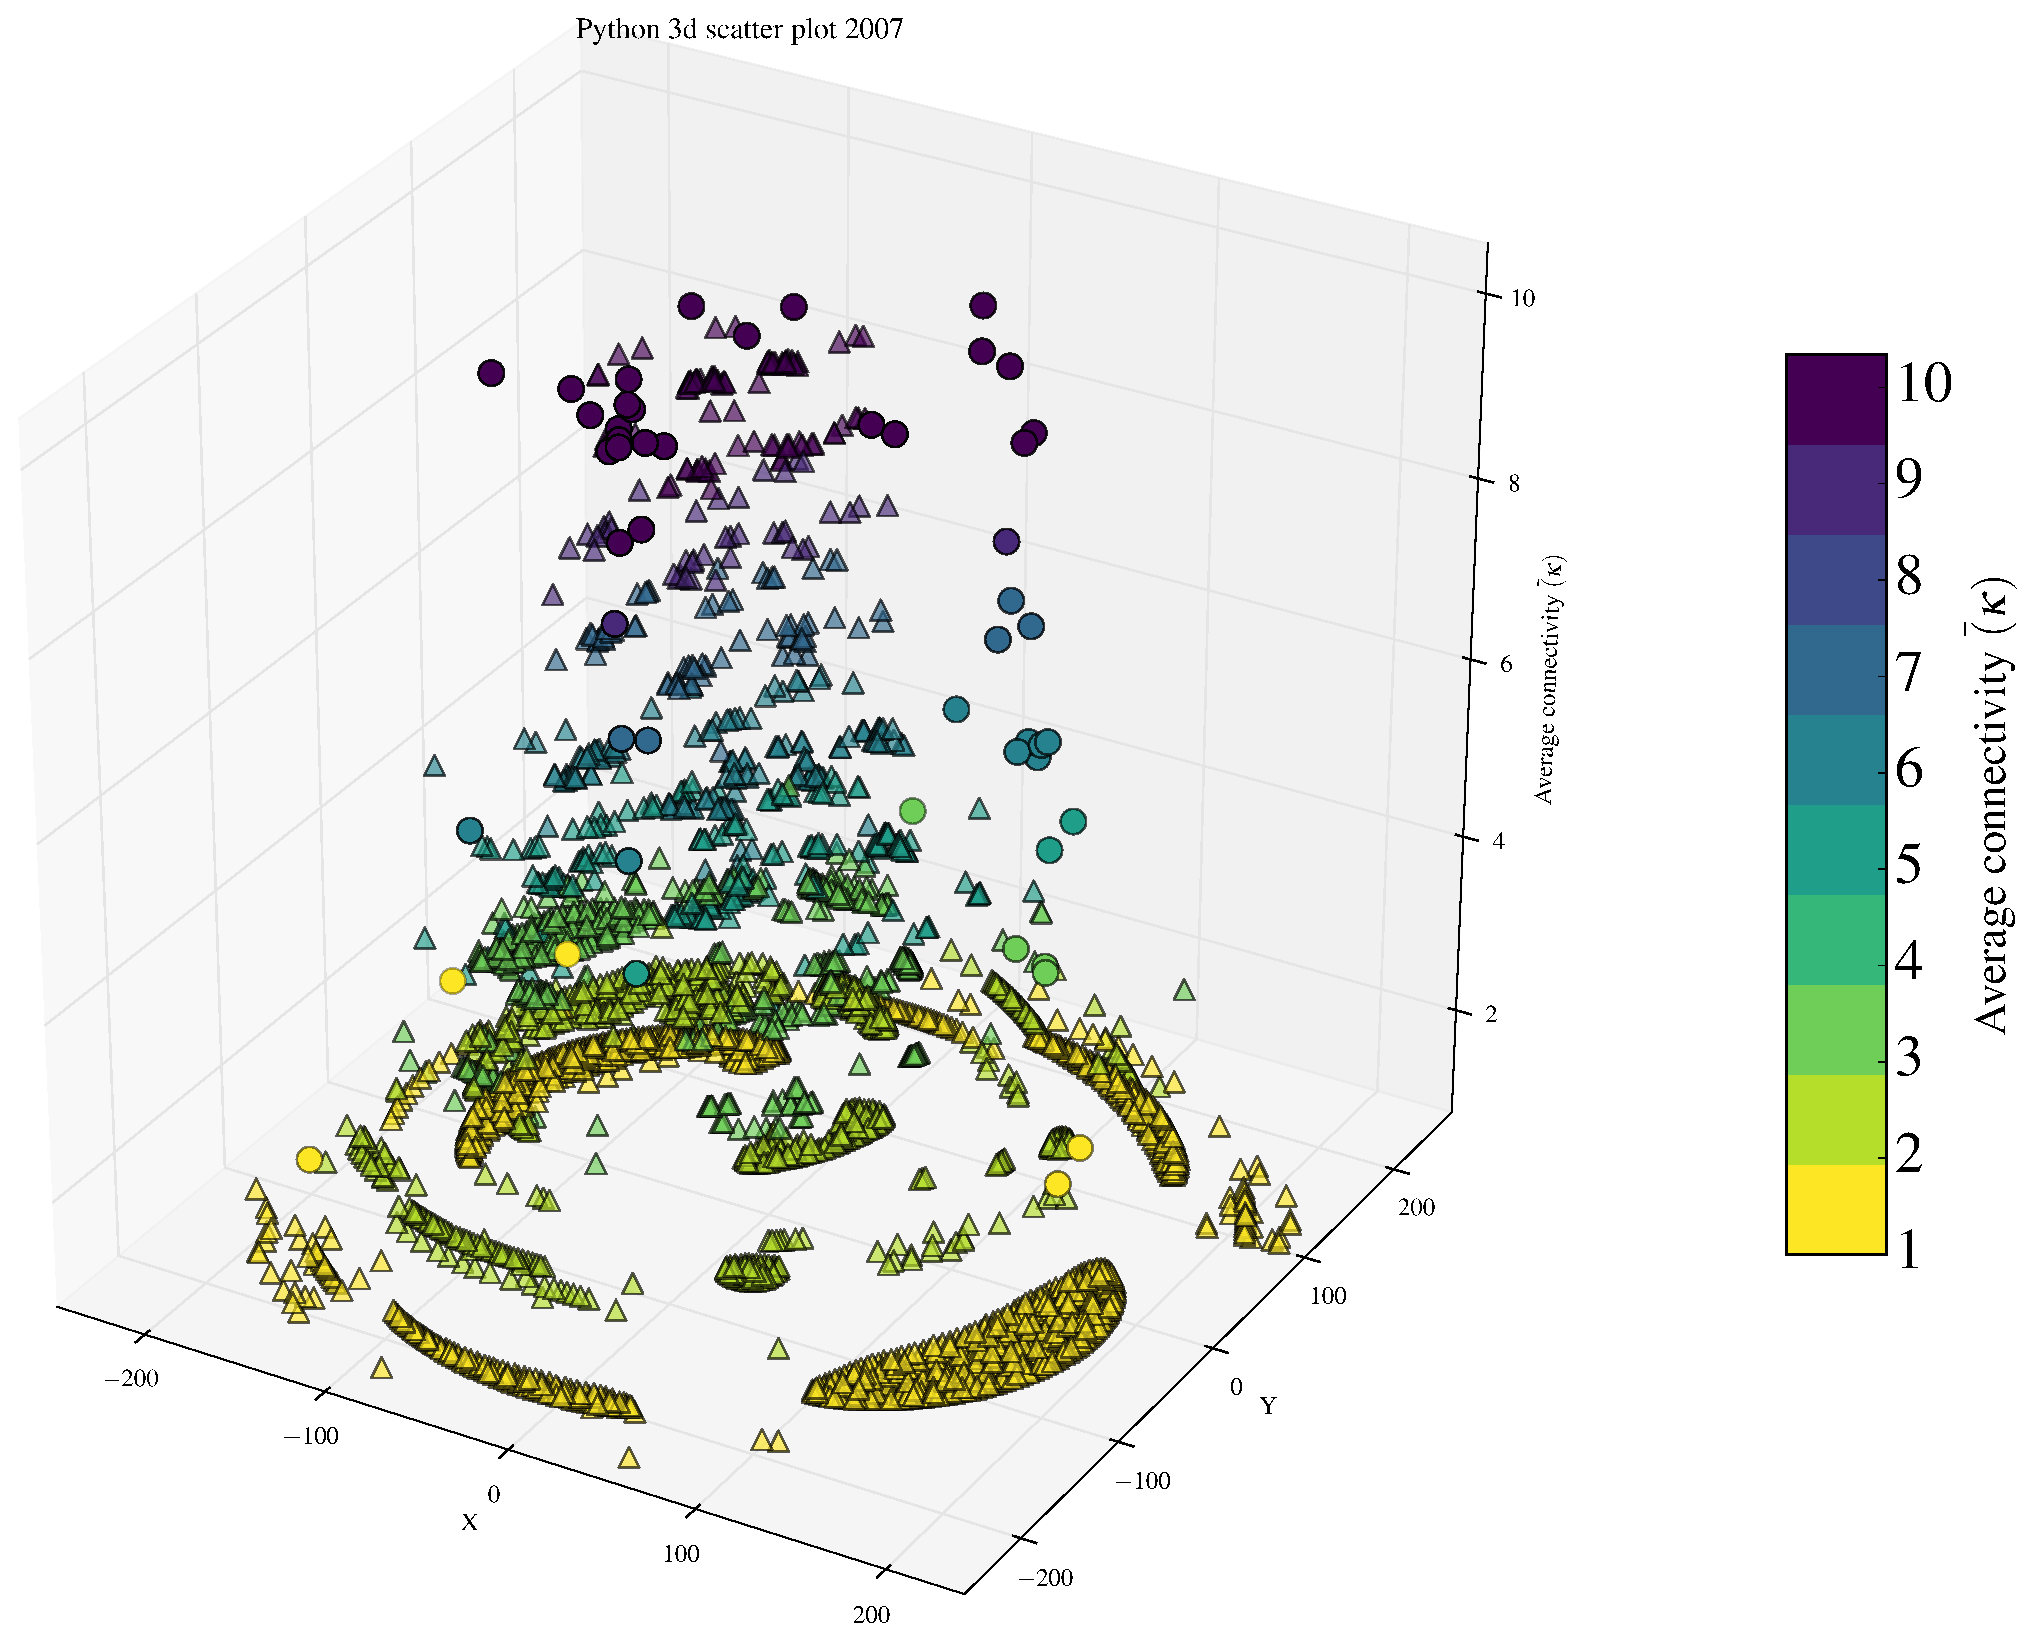
\includegraphics[scale=0.25]{img/3d_scatter_python_2007}
\end{center}

\end{frame}

\begin{frame}
\frametitle{Graphical Representation of the Structural Cohesion Analysis}

\begin{center}
\textbf{Python Cooperation Network 2008 (59 developers)}
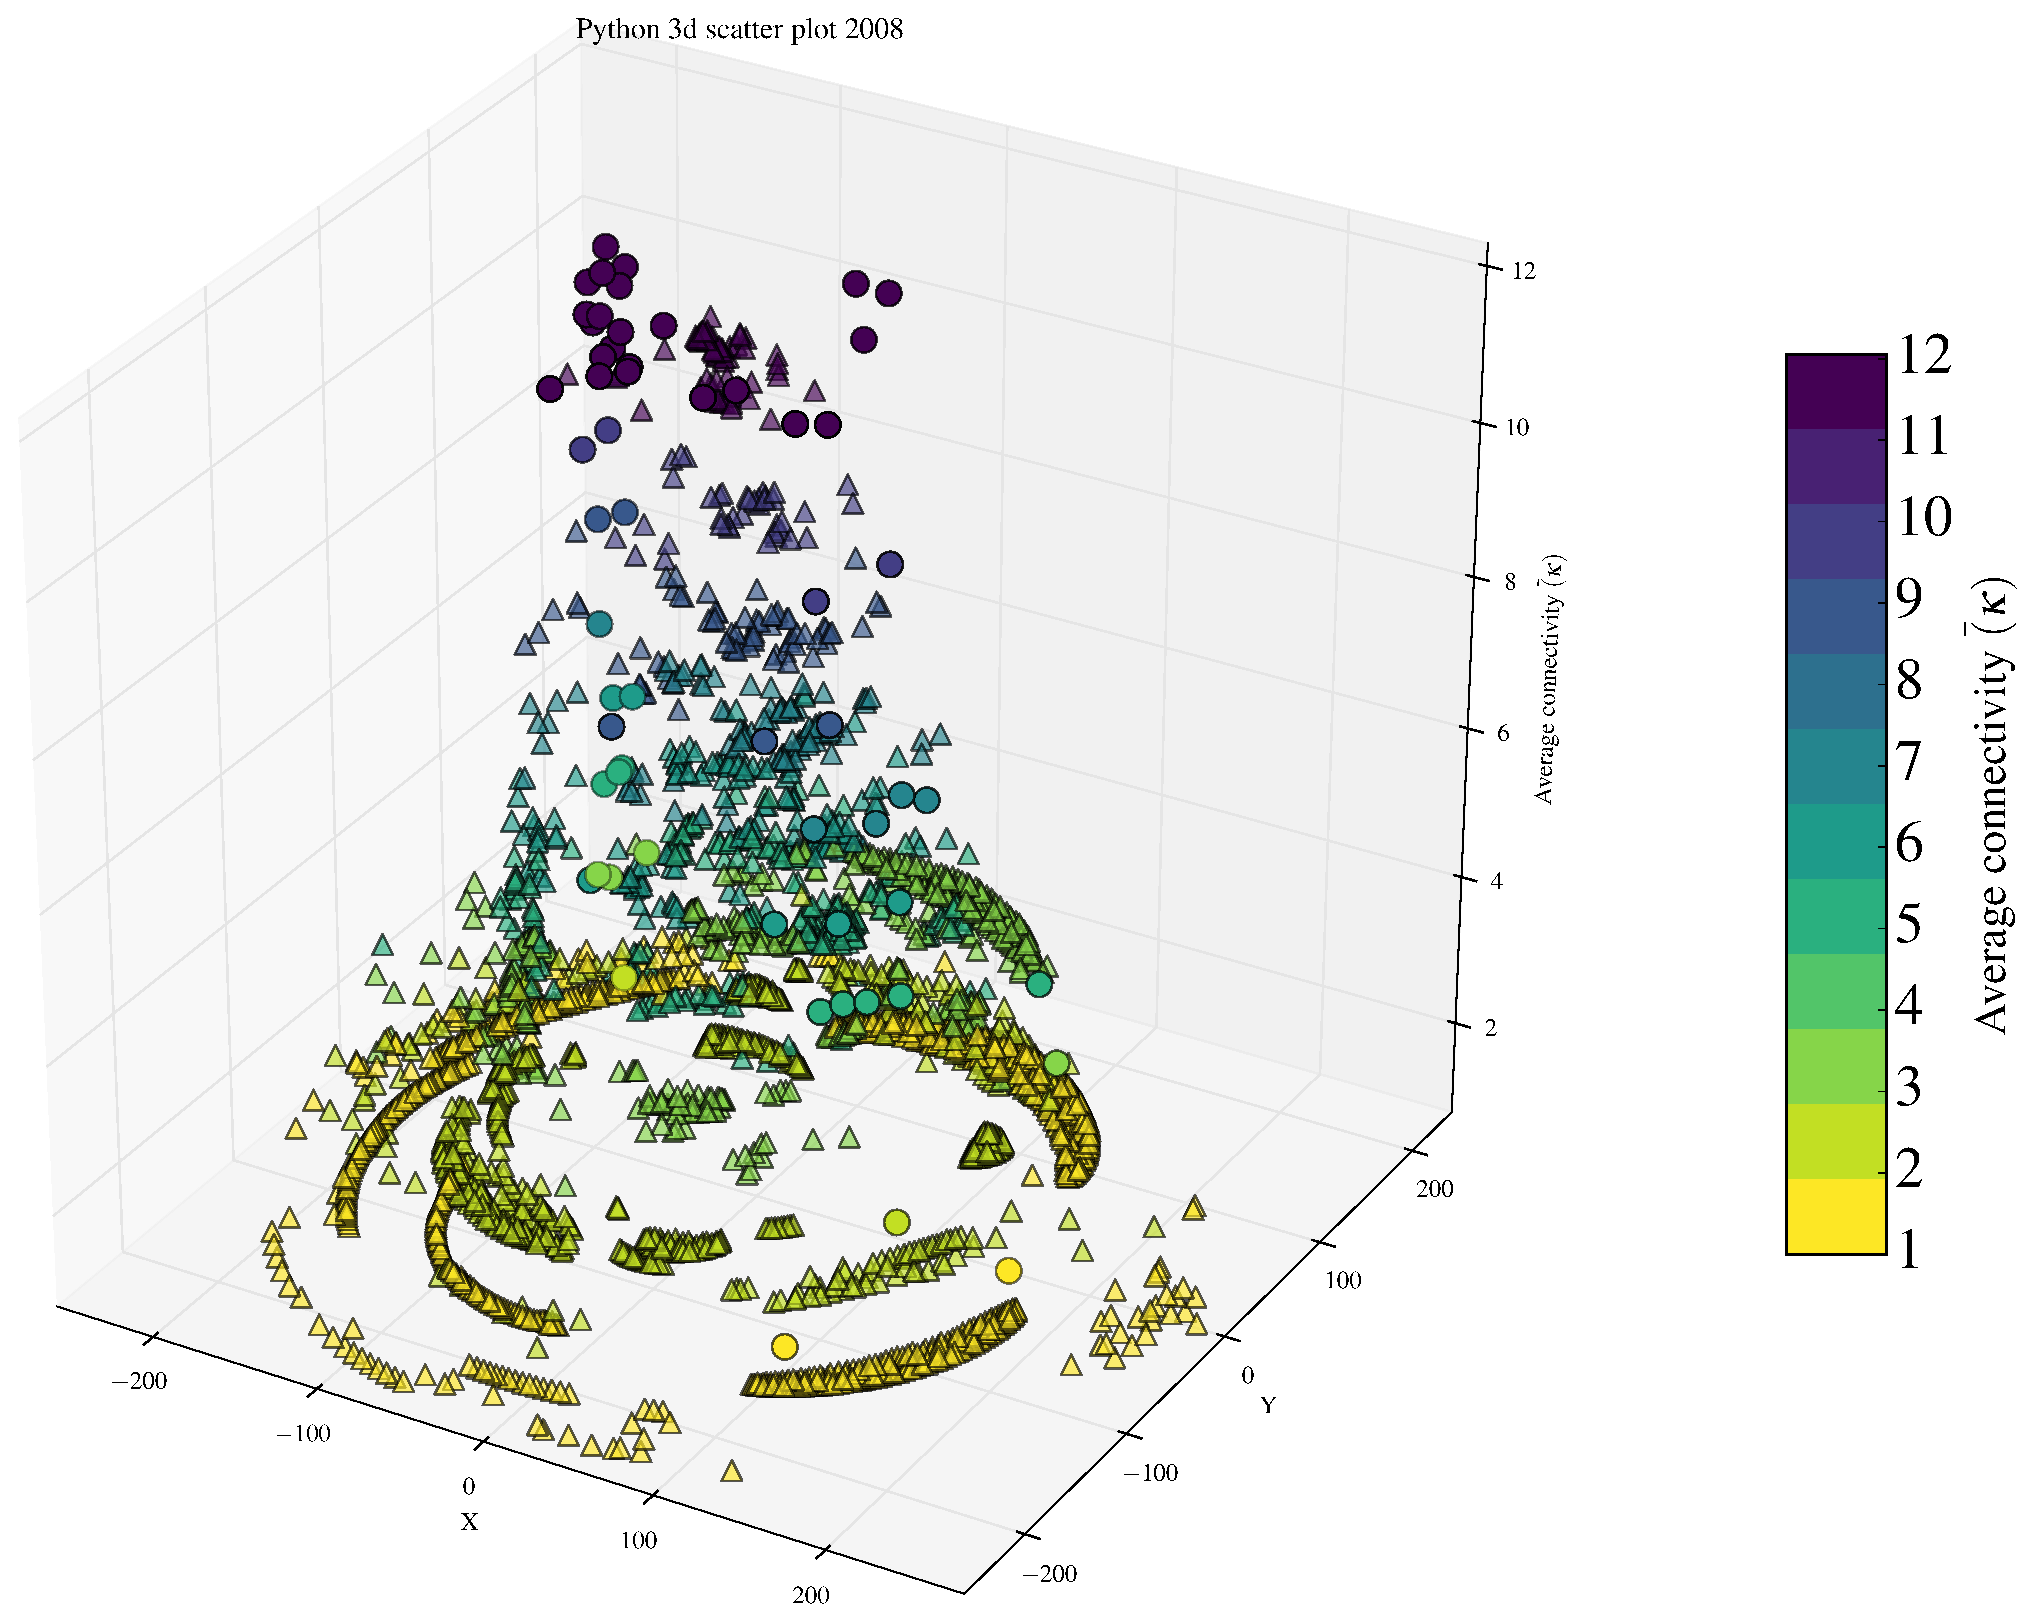
\includegraphics[scale=0.25]{img/3d_scatter_python_2008}
\end{center}

\end{frame}

\begin{frame}
\frametitle{Graphical Representation of the Structural Cohesion Analysis}

\begin{center}
\textbf{Python Cooperation Network 2009 (58 developers)}
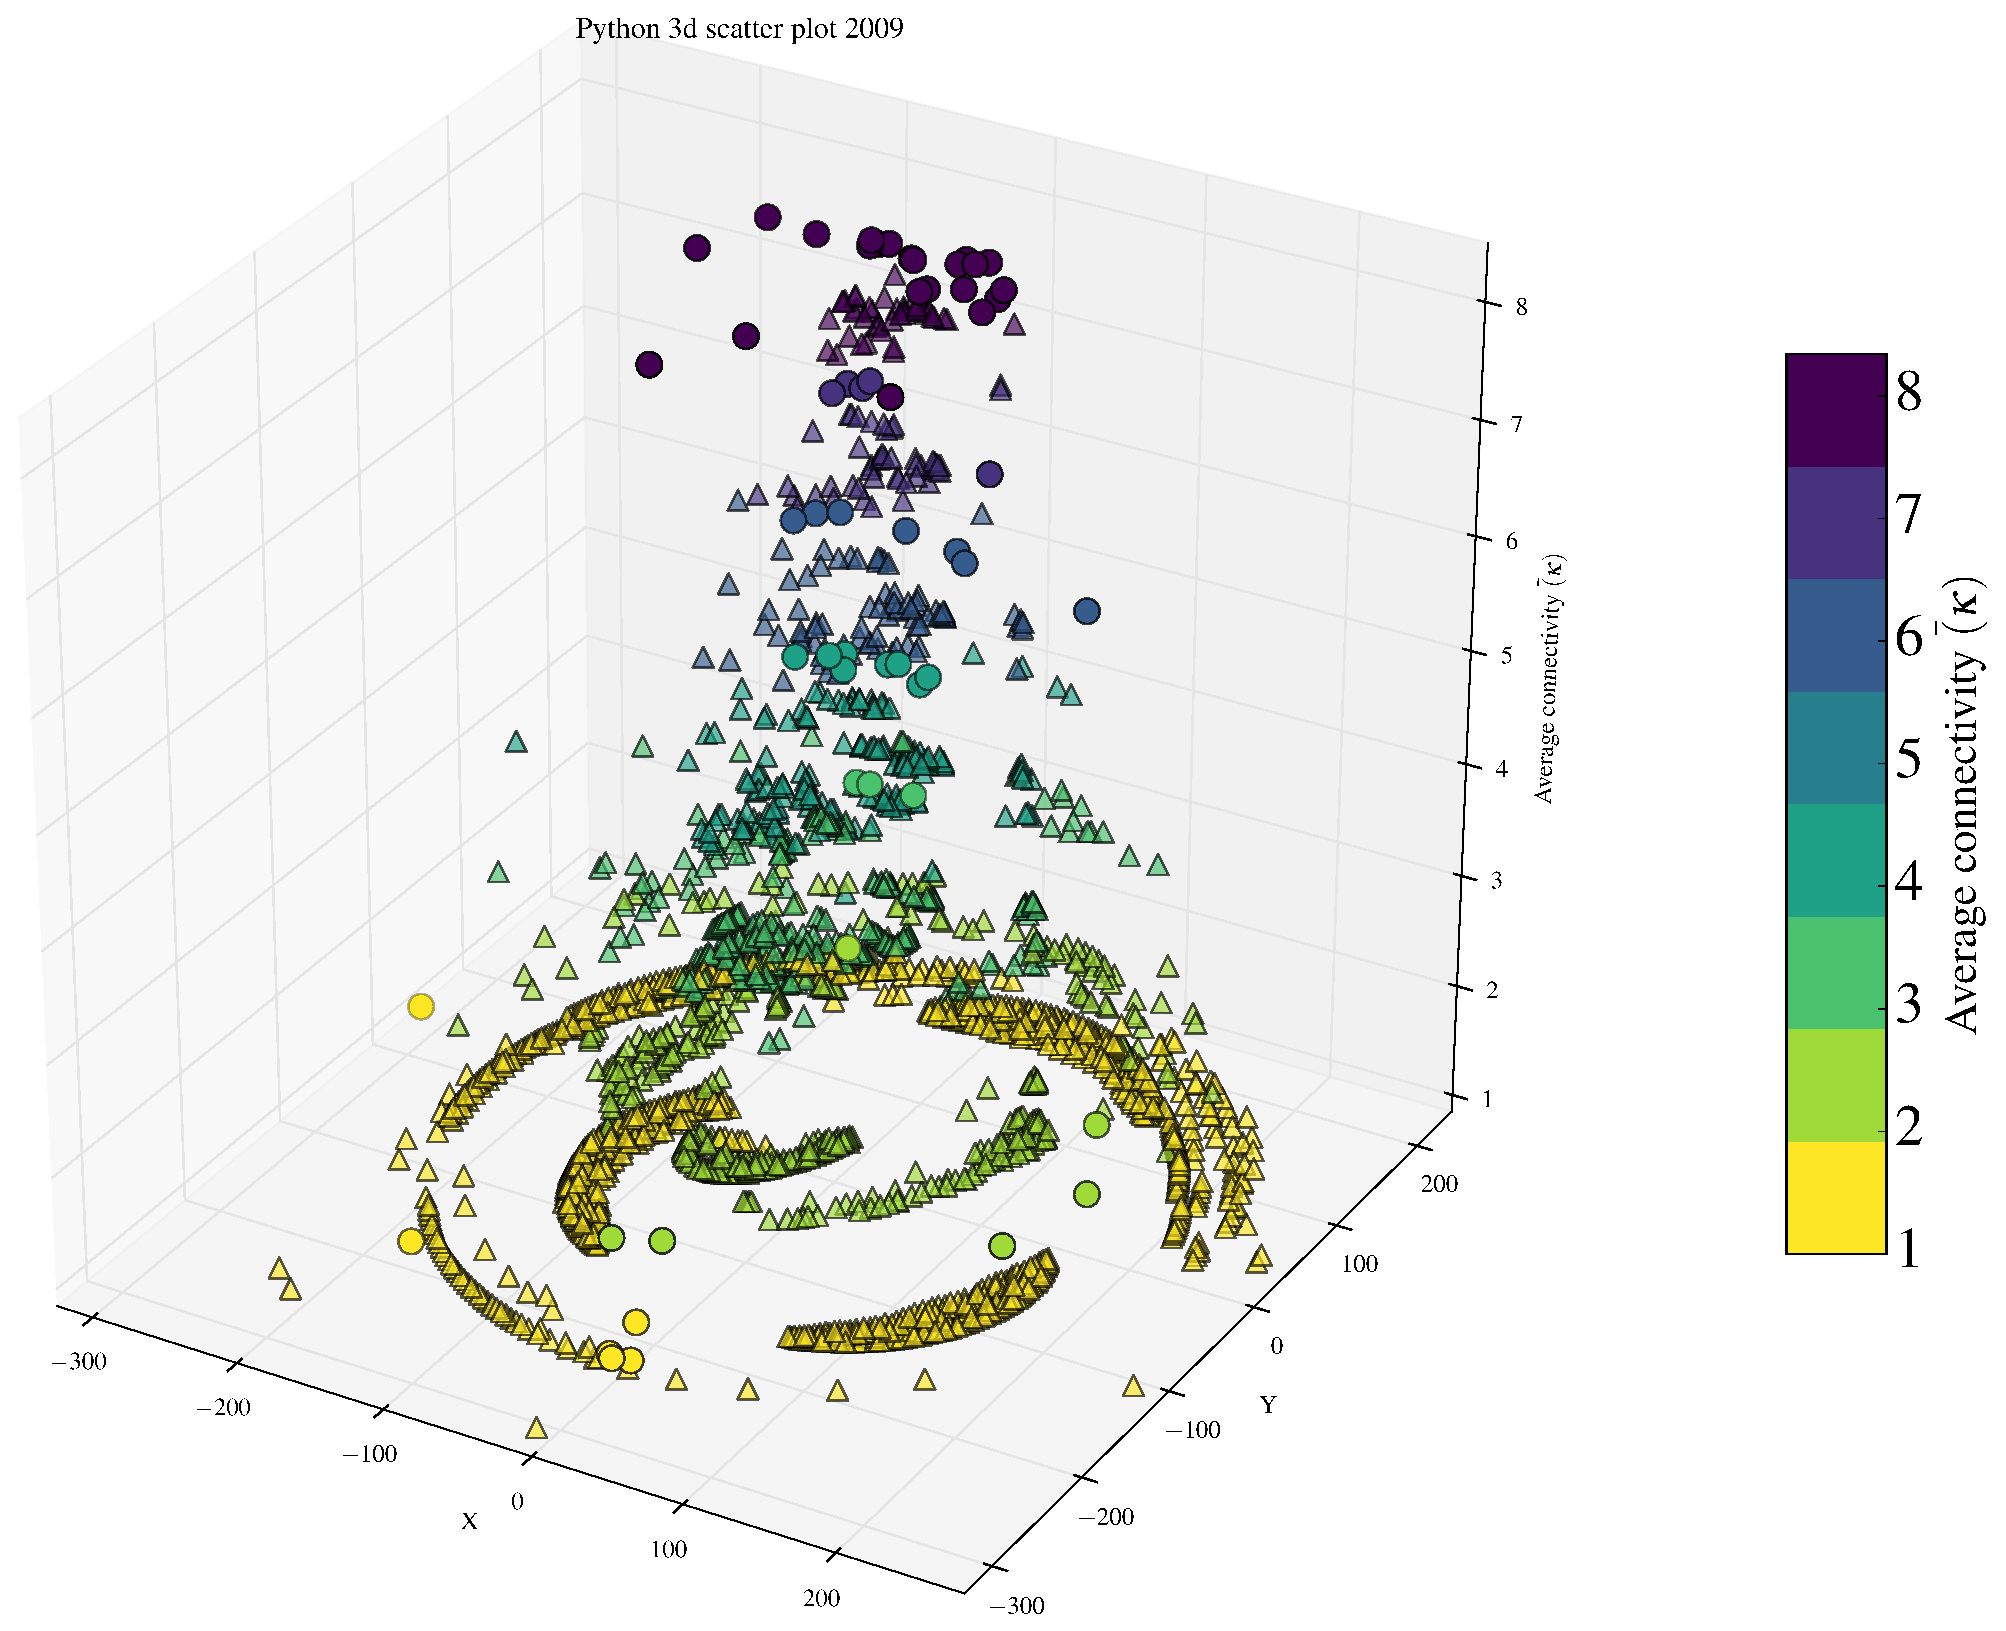
\includegraphics[scale=0.25]{img/3d_scatter_python_2009}
\end{center}

\end{frame}


\begin{frame}
\frametitle{Graphical Representation of the Structural Cohesion Analysis}

\begin{center}
\textbf{Python Cooperation Network 2010 (63 developers)}
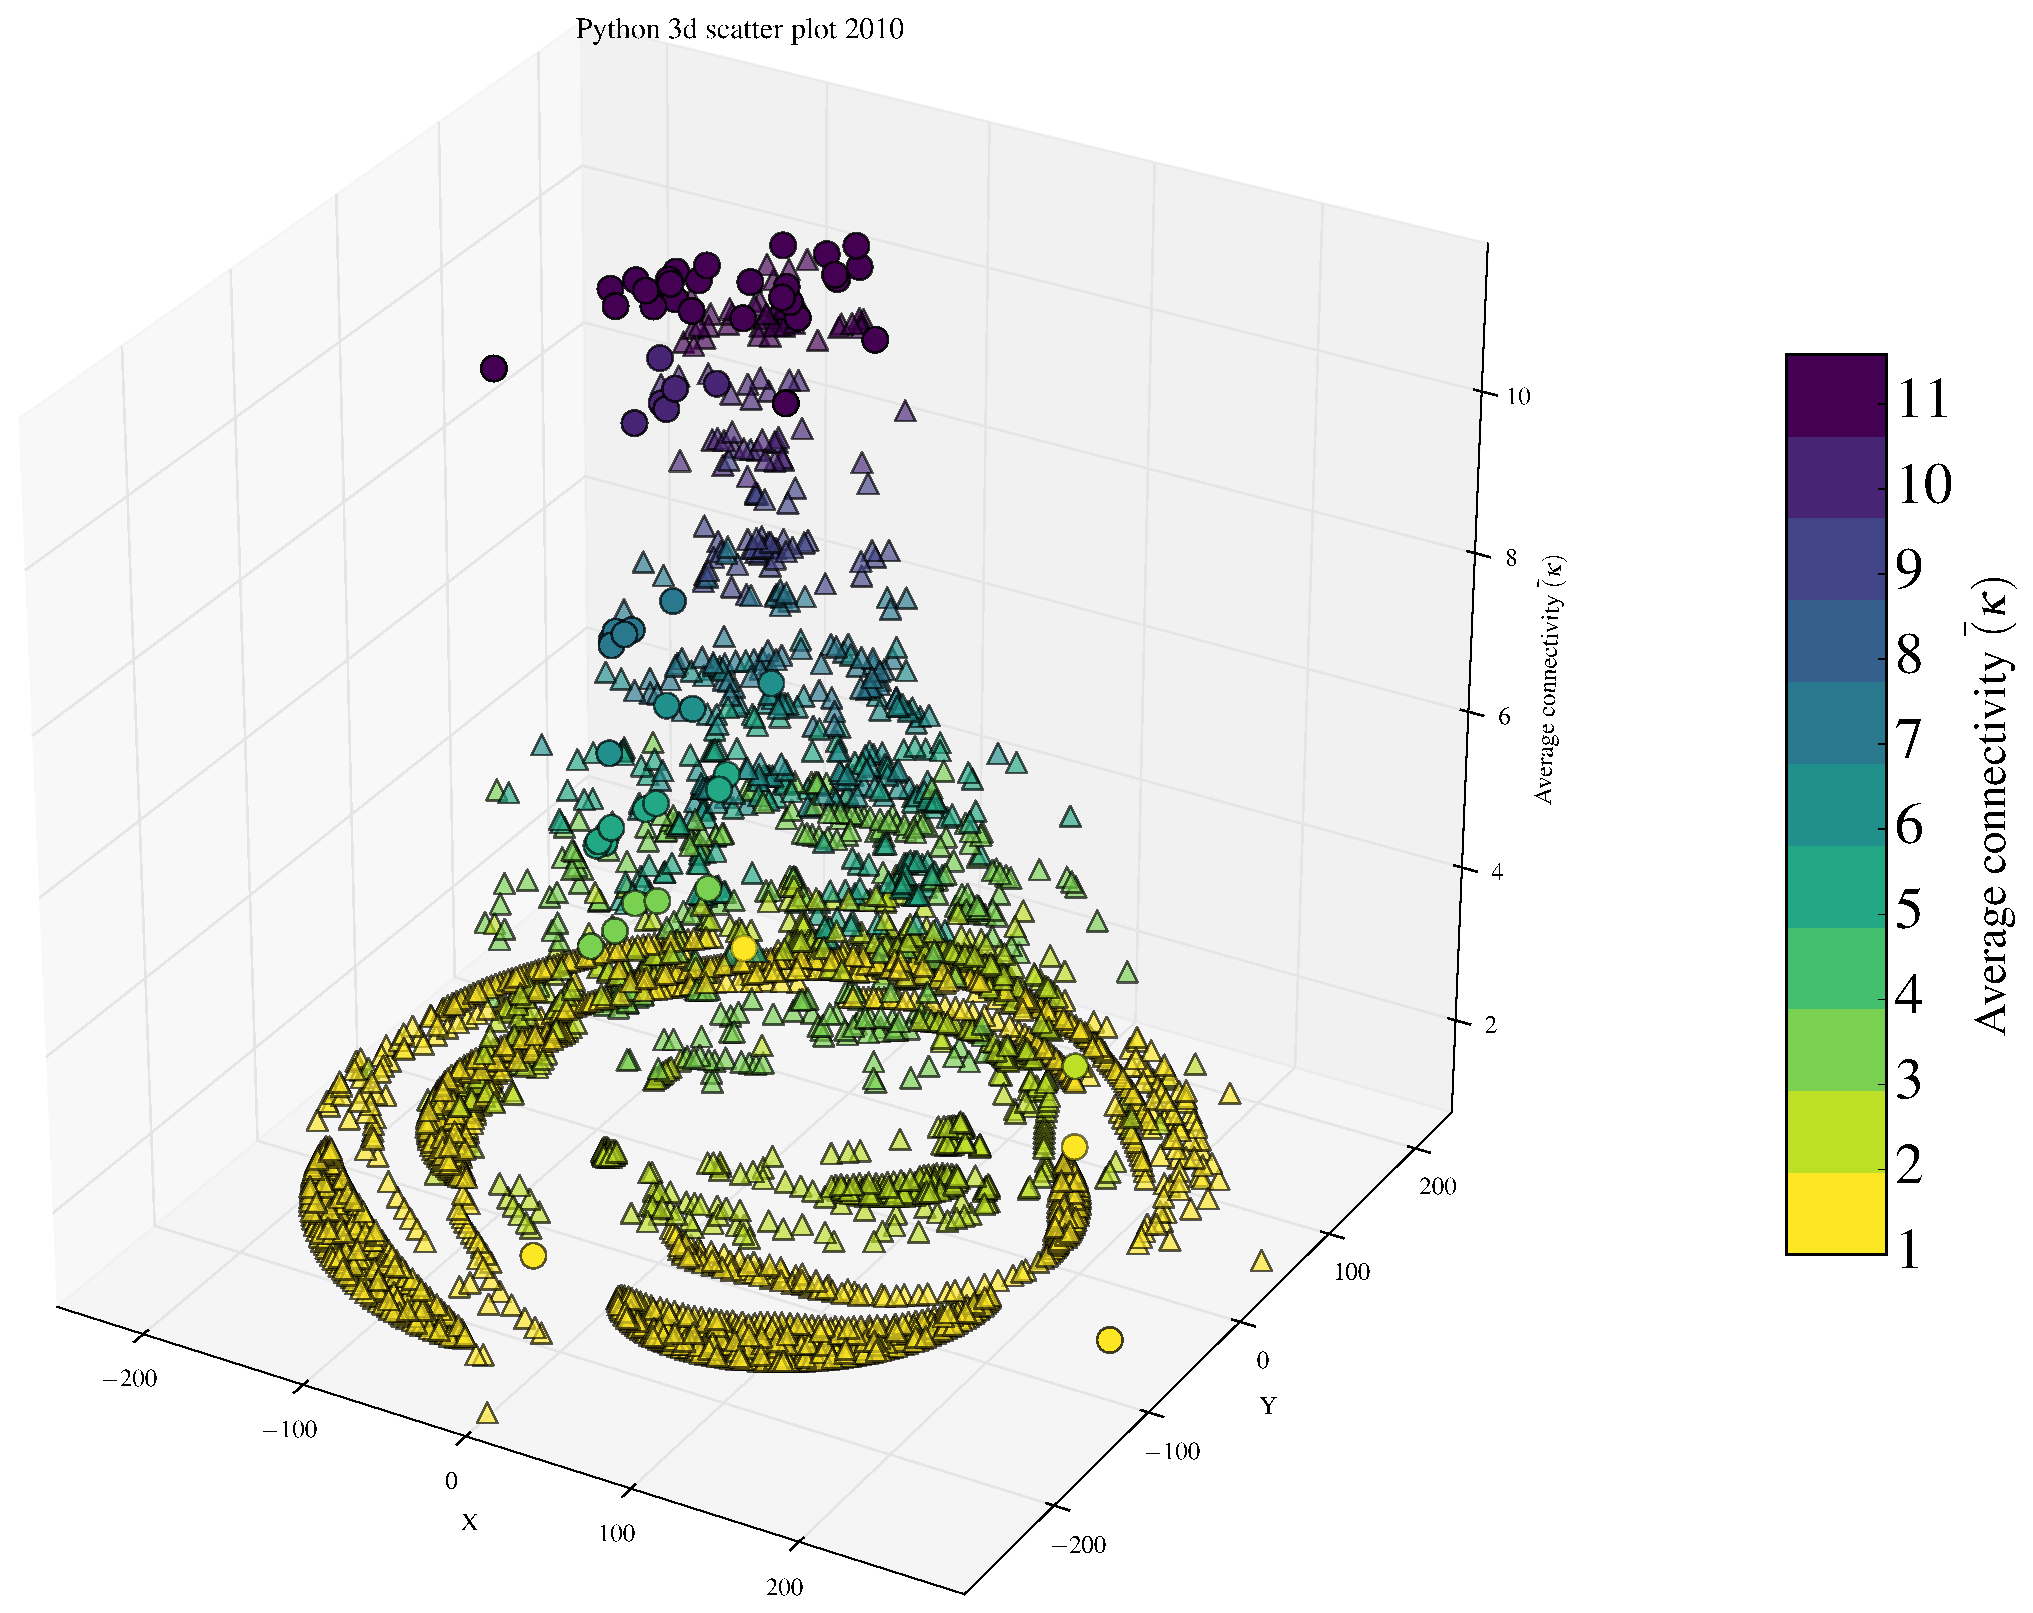
\includegraphics[scale=0.25]{img/3d_scatter_python_2010}
\end{center}

\end{frame}

\begin{frame}
\frametitle{Graphical Representation of the Structural Cohesion Analysis}

\begin{center}
\textbf{Python Cooperation Network 2011 (63 developers)}
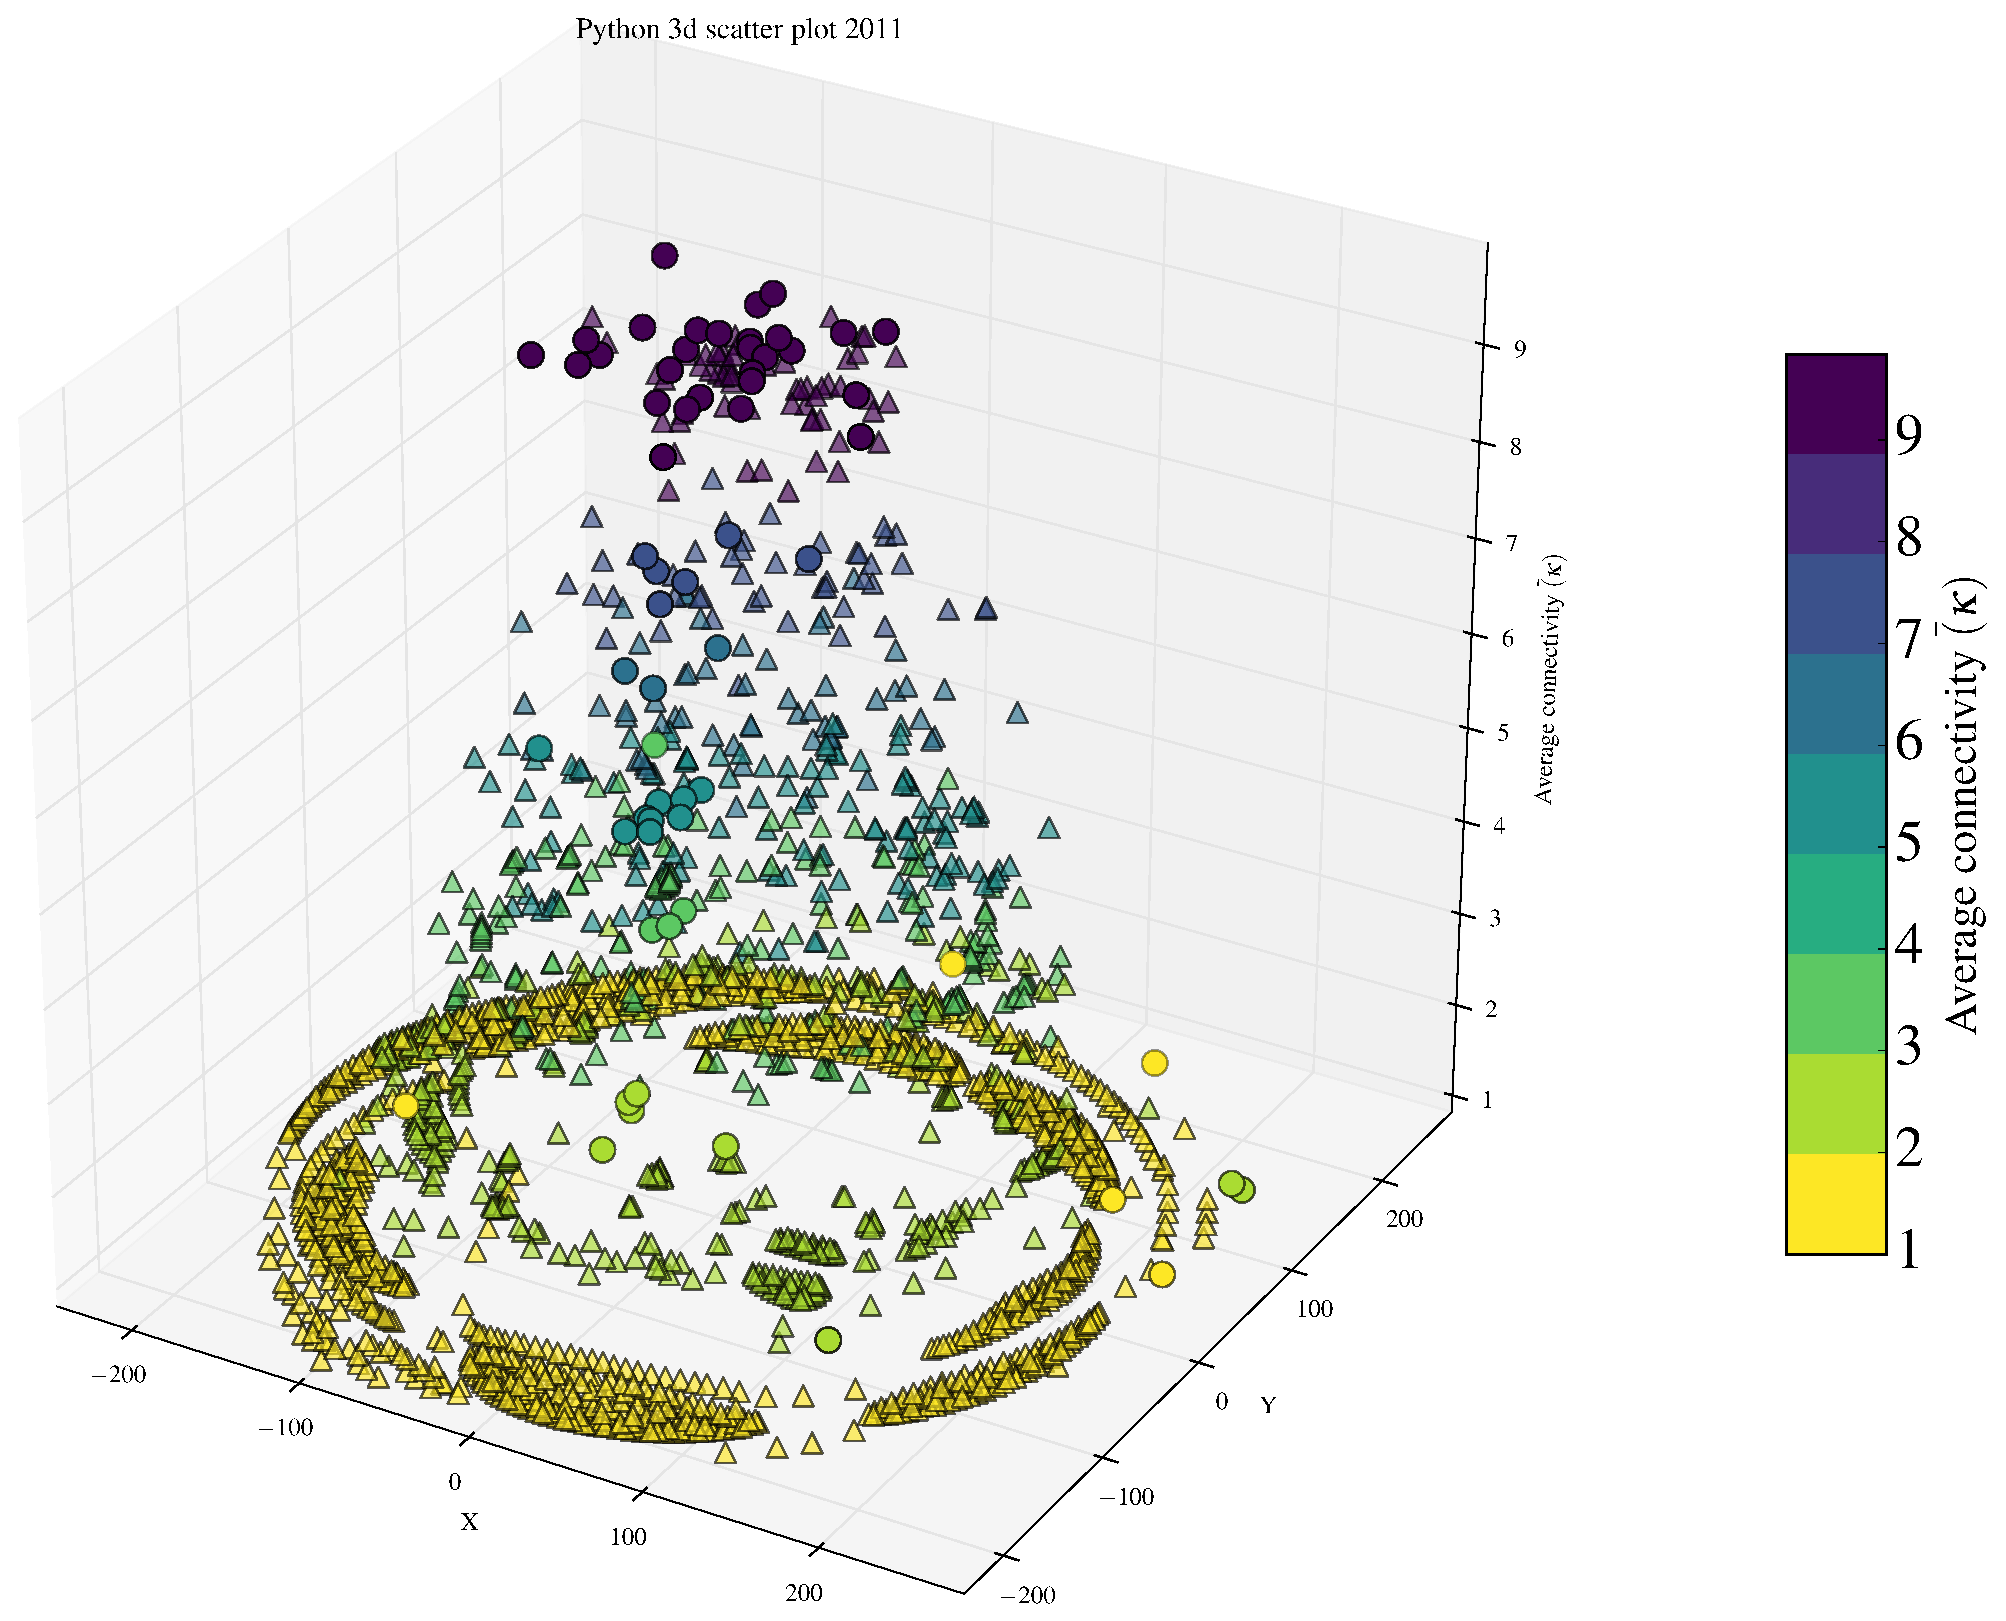
\includegraphics[scale=0.25]{img/3d_scatter_python_2011}
\end{center}

\end{frame}

\begin{frame}
\frametitle{Graphical Representation of the Structural Cohesion Analysis}

\begin{center}
\textbf{Python Cooperation Network 2012 (65 developers)}
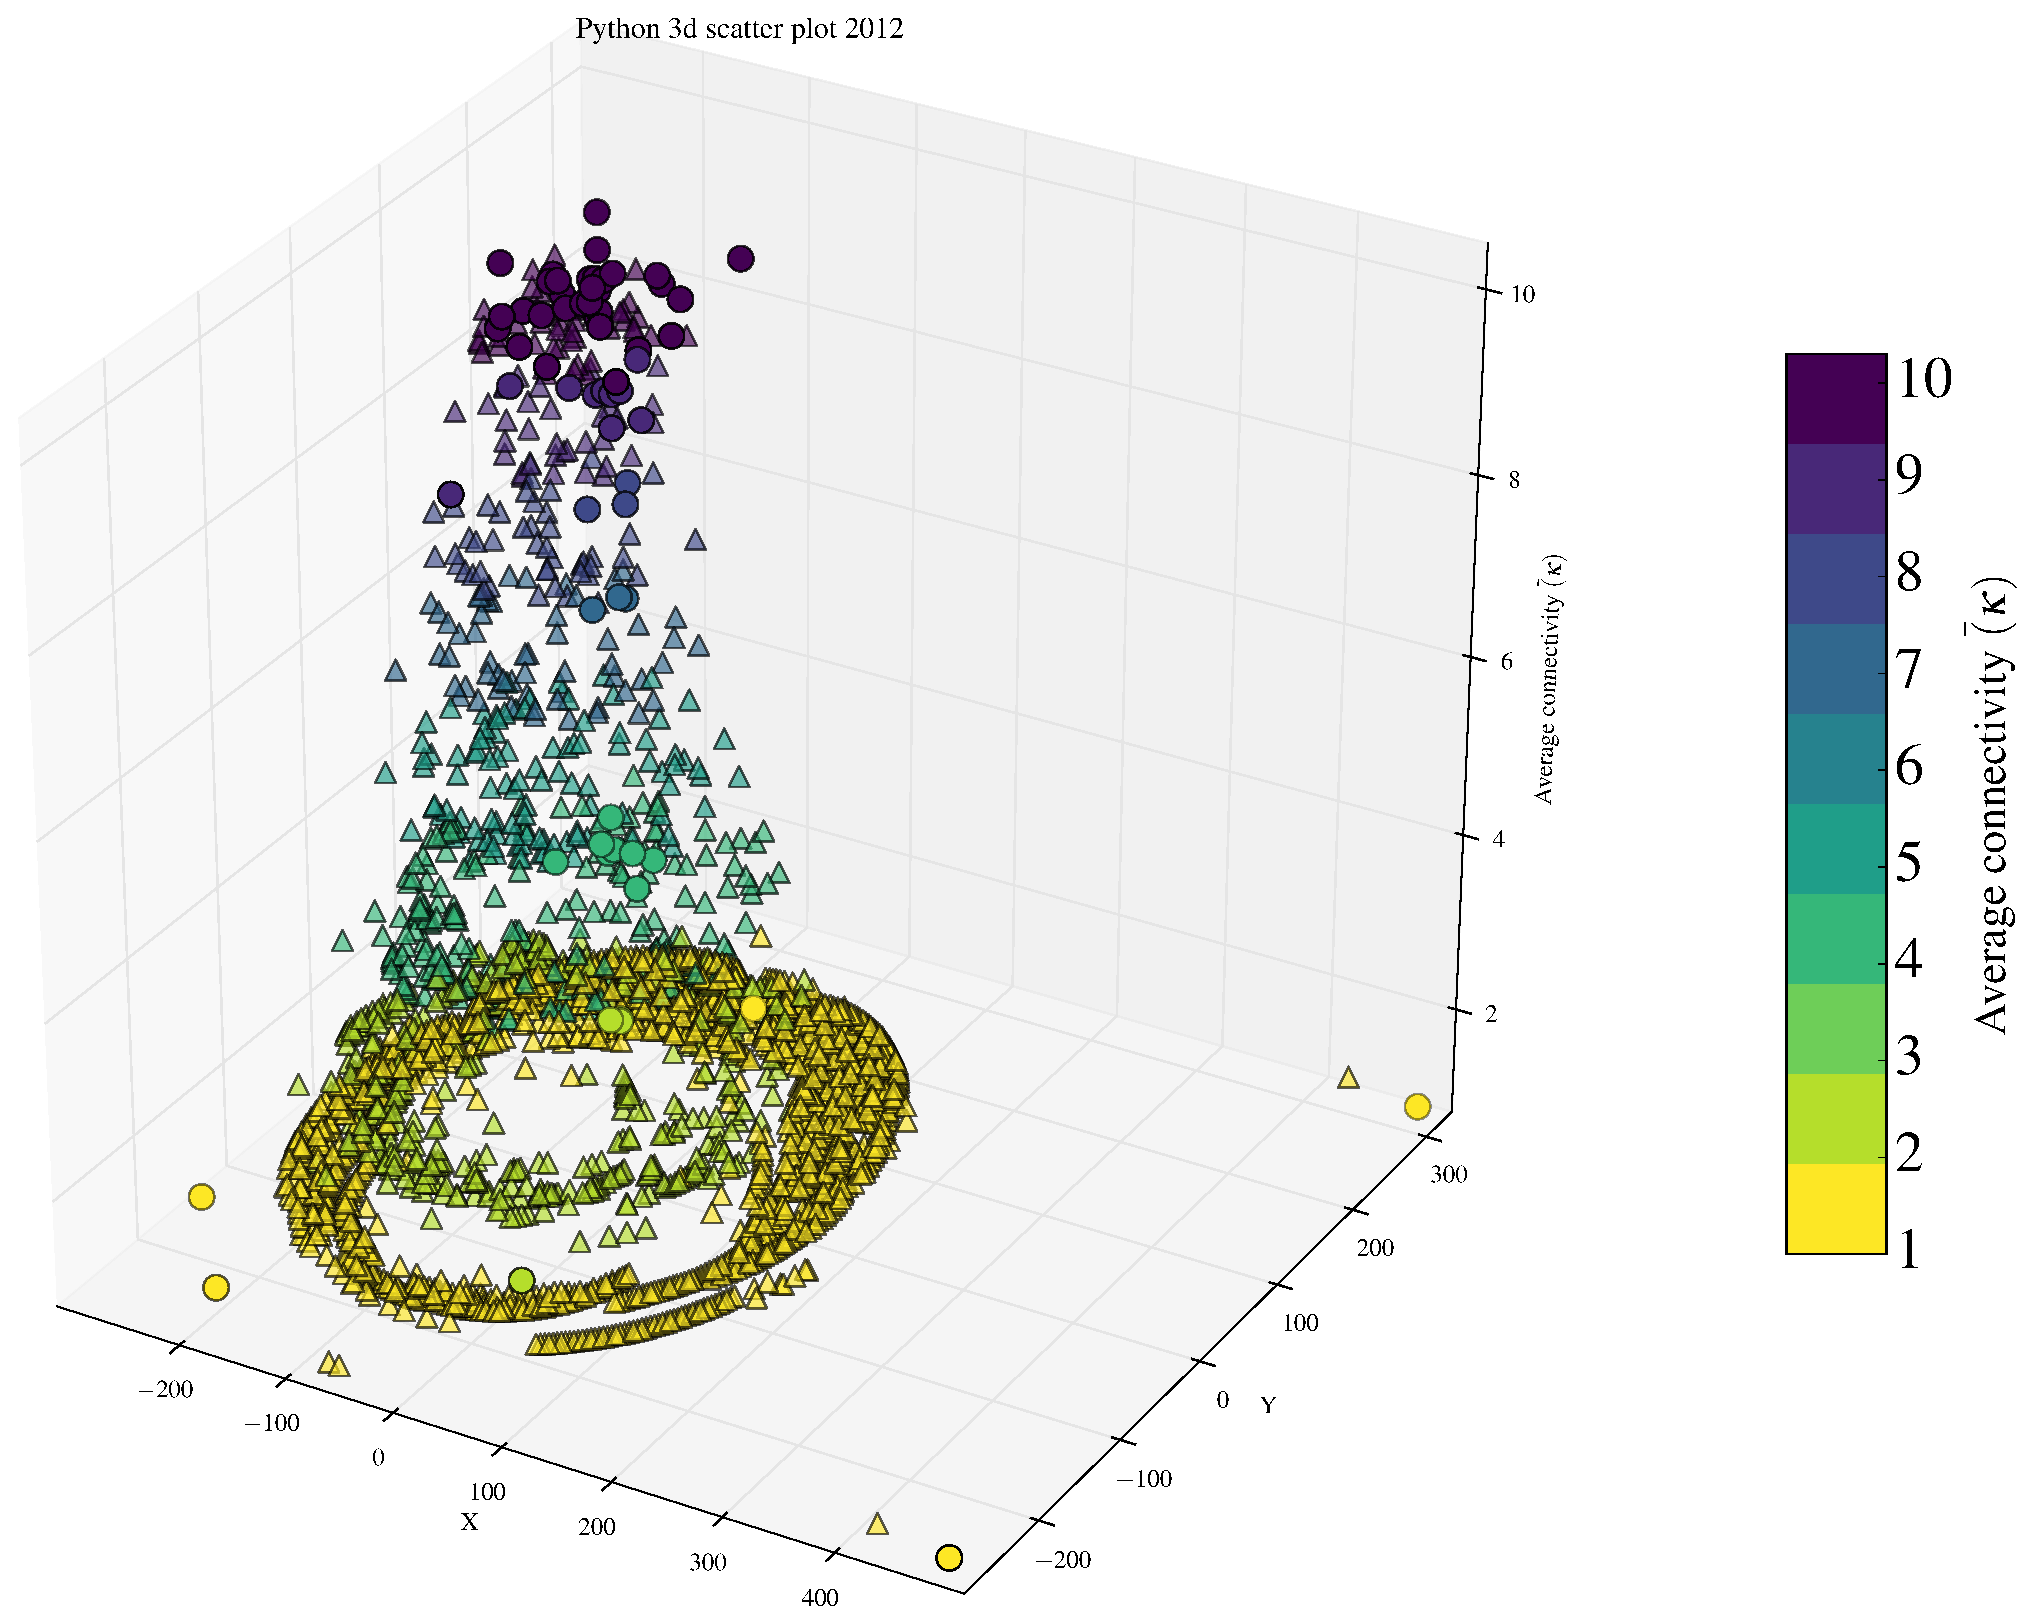
\includegraphics[scale=0.25]{img/3d_scatter_python_2012}
\end{center}

\end{frame}


\begin{frame}
\frametitle{Graphical Representation of the Structural Cohesion Analysis}

\begin{center}
\textbf{Python Cooperation Network 2013 (63 developers)}
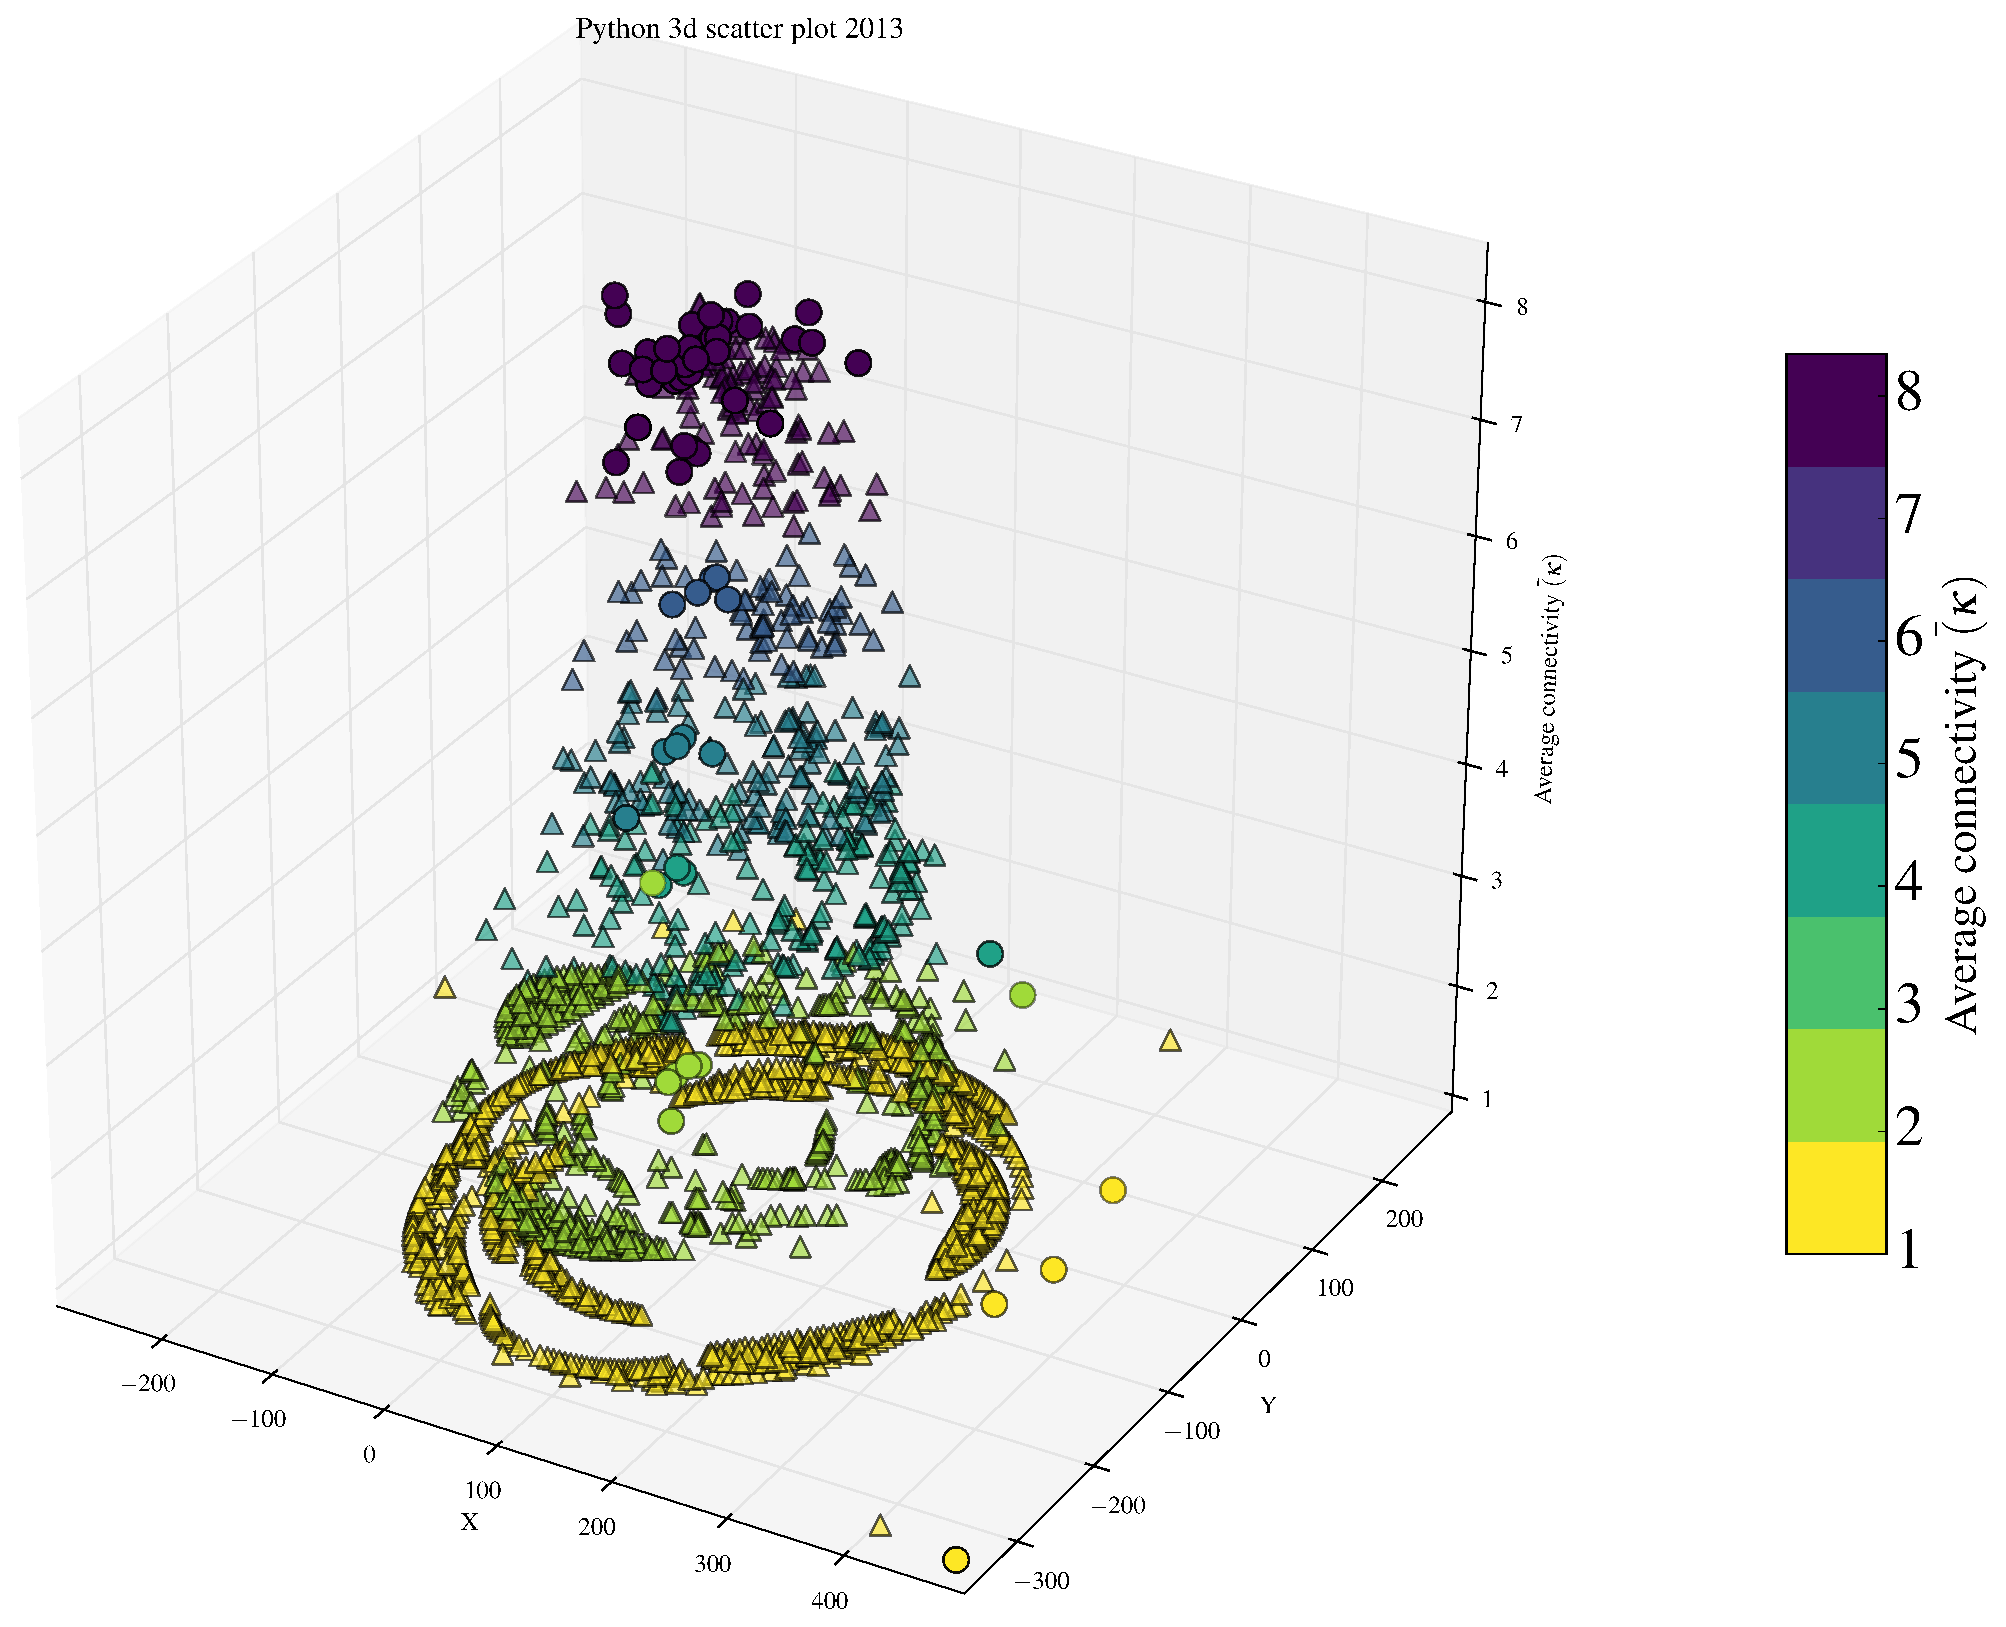
\includegraphics[scale=0.25]{img/3d_scatter_python_2013}
\end{center}

\end{frame}

\begin{frame}
\frametitle{Graphical Representation of the Structural Cohesion Analysis}

\begin{center}
\textbf{Python Cooperation Network 2014 (62 developers)}
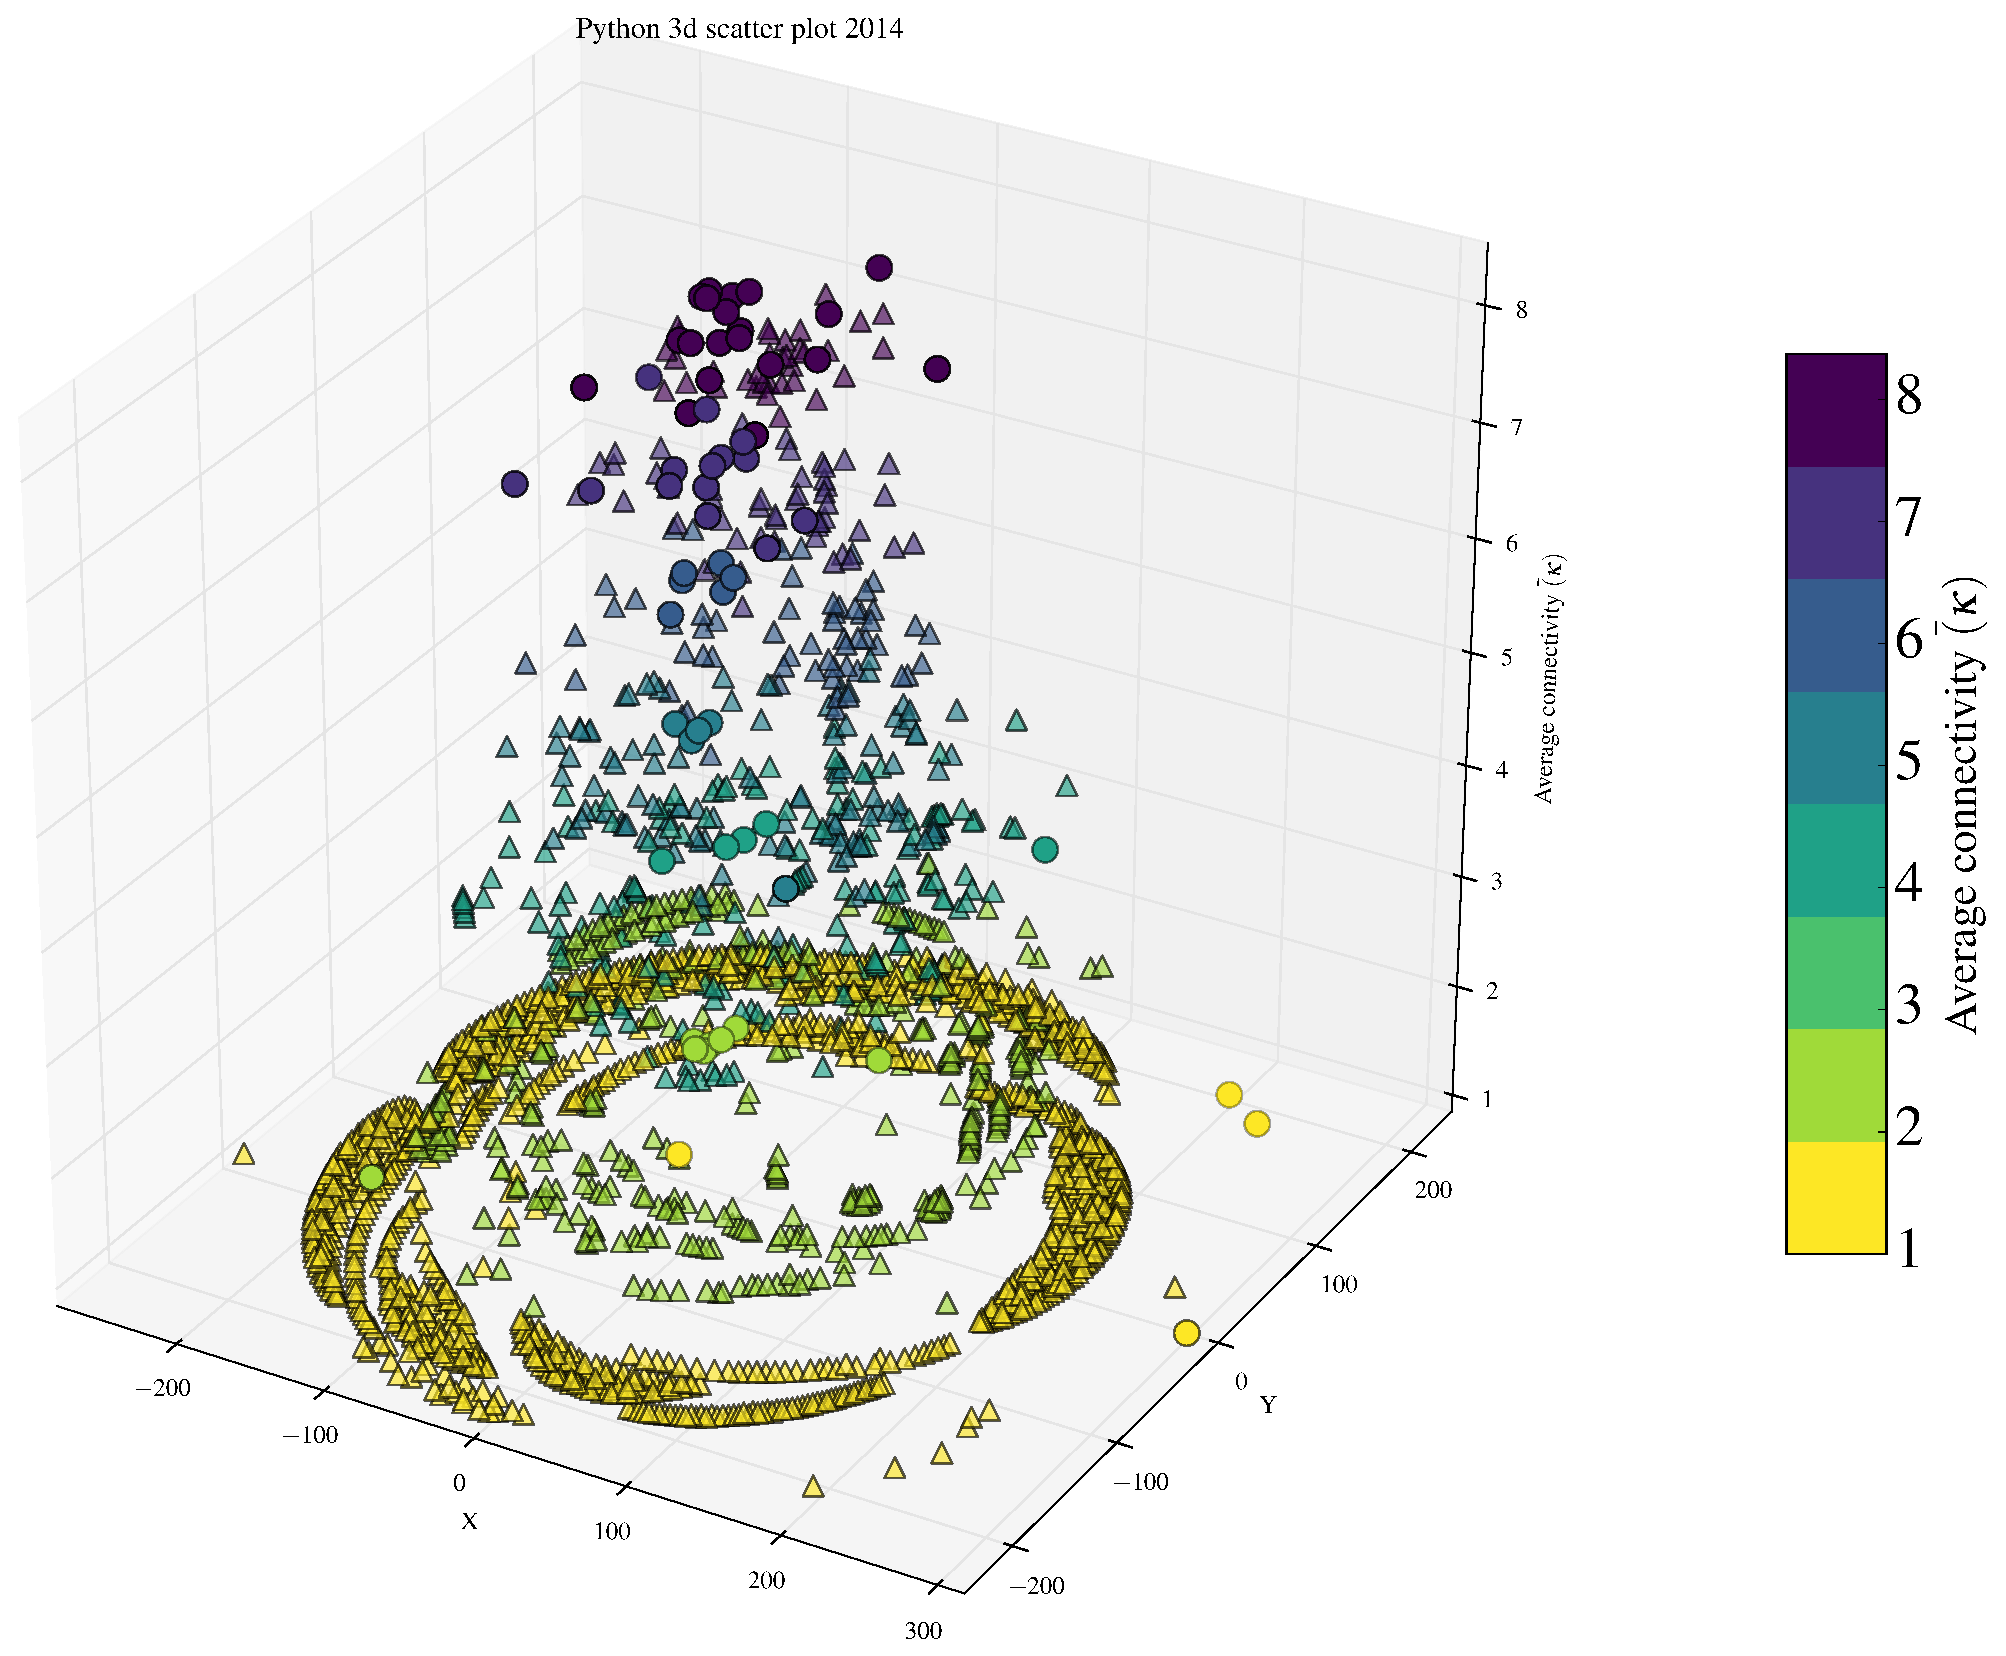
\includegraphics[scale=0.25]{img/3d_scatter_python_2014}
\end{center}

\end{frame}


\begin{frame}
\frametitle{Comparison with null models}

\begin{columns}[c]
\begin{column}{0.5\textwidth}
\begin{center}
\textbf{Actual Cooperation Network 2004}
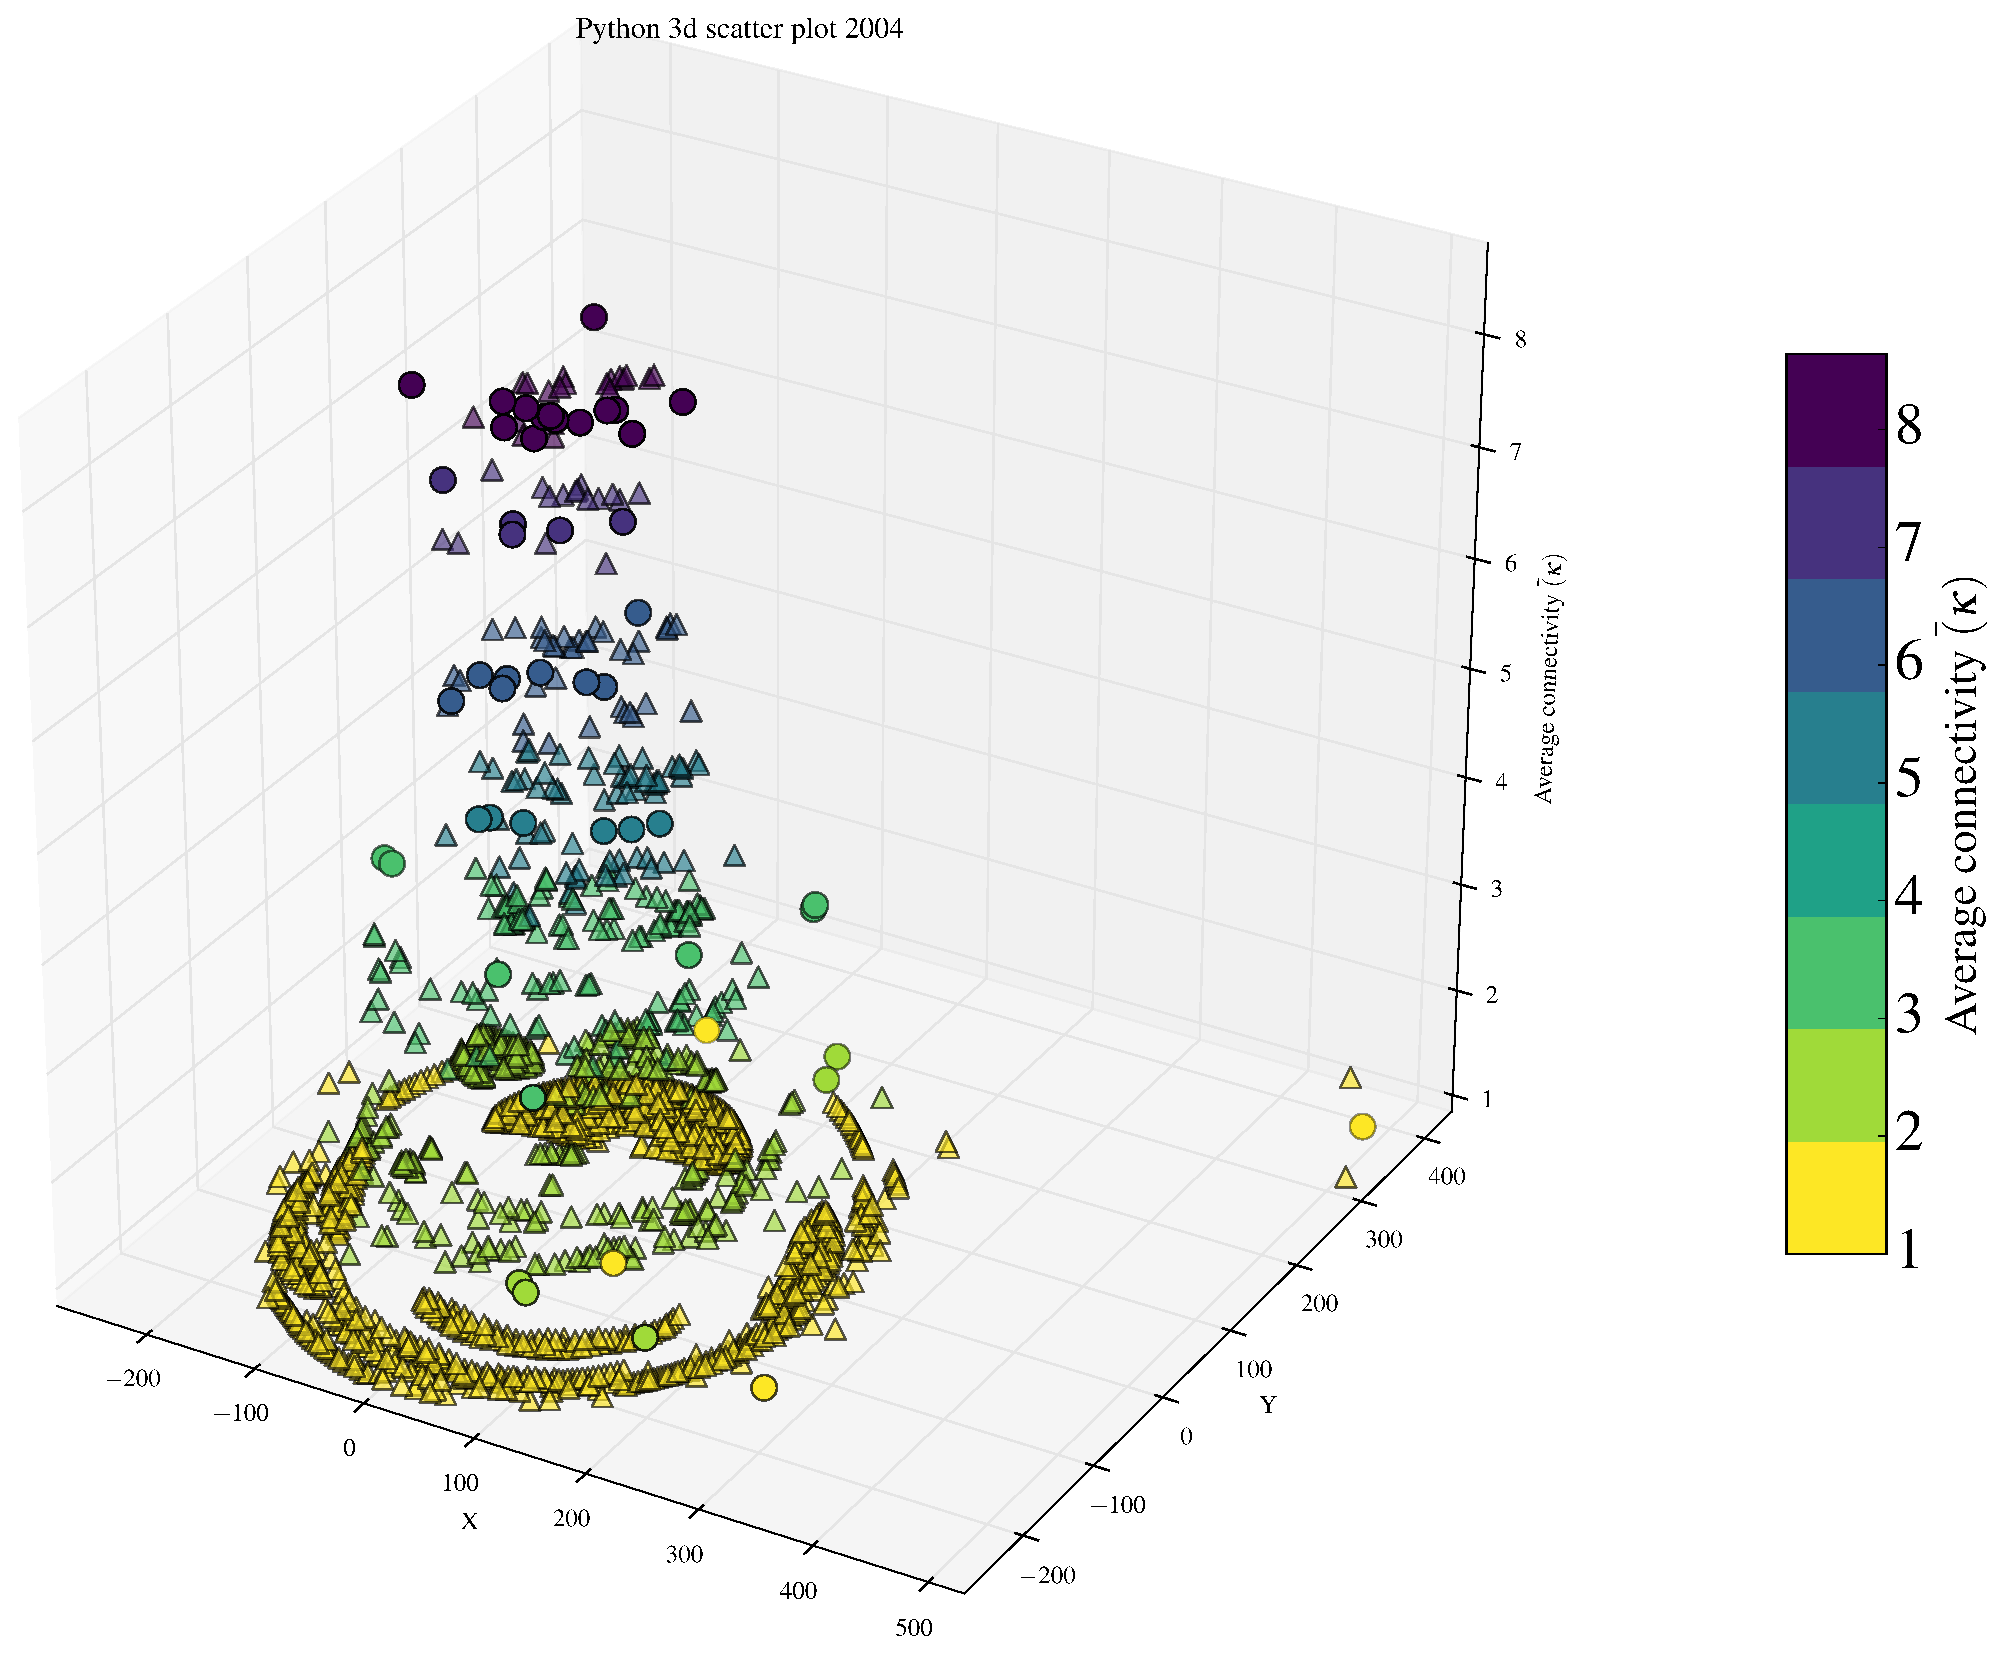
\includegraphics[scale=0.16]{../../figures/3d_scatter_python_2004}
\end{center}
\end{column}

\begin{column}{0.5\textwidth}
\begin{center}
\textbf{Null model}
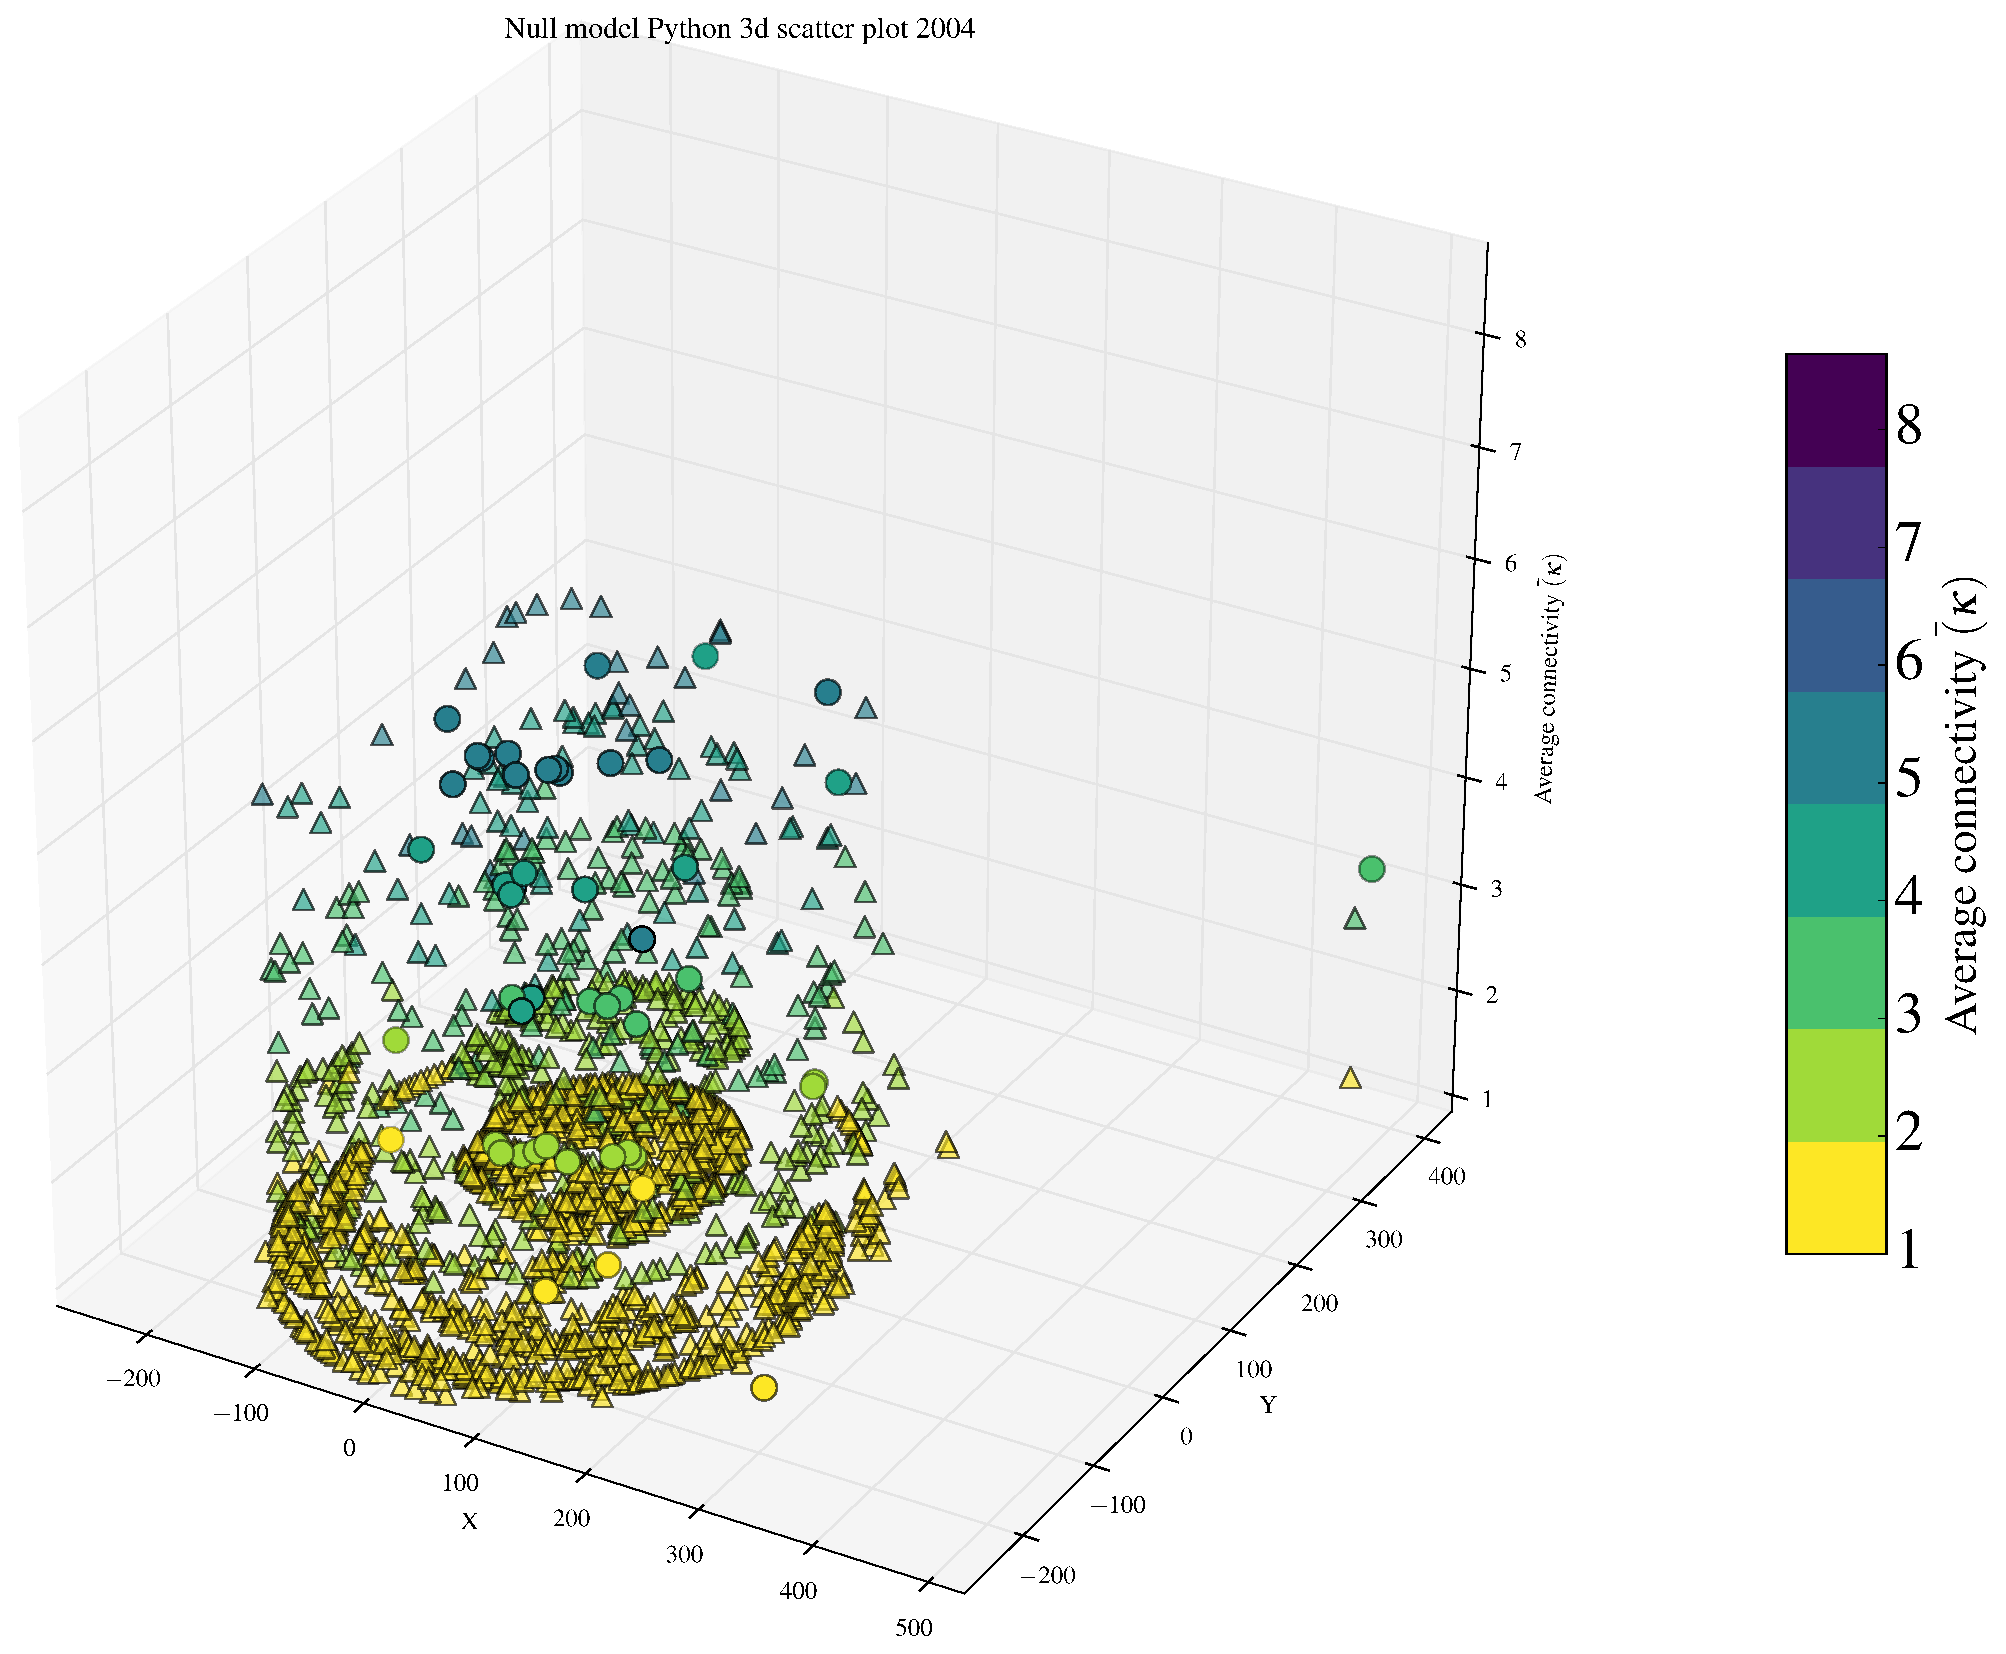
\includegraphics[scale=0.16]{../../figures/3d_scatter_python_2004_null}
\end{center}
\end{column}
\end{columns}

\end{frame}


\section{Connectivity Hierarchy and Individual Contributions}

\begin{frame}
\frametitle{Individual contributions by connectivity level}

\begin{itemize}
\item The developers that contribute the most are in the higher levels of the connectivity structure of the project's cooperation networks.

\item The hierarchical connectivity structure shapes the volume of contribution of individual developers.

\end{itemize}

\begin{figure}
\vspace{-0.6cm}
\centering
\subfloat[Python: developer \% by connectivity level]{
\label{}
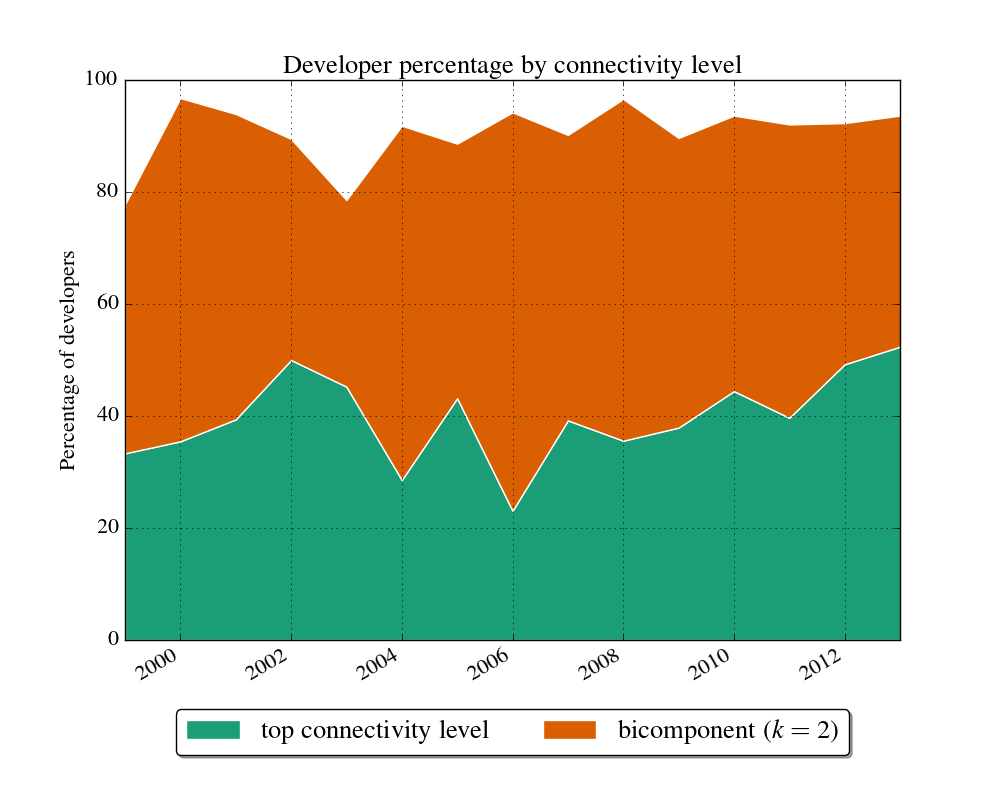
\includegraphics[scale=0.2]{../../figures/evolution_developers_python_years}
}
\hspace{0.02cm}
\subfloat[Python: contributions by connectivity level]{
\label{}
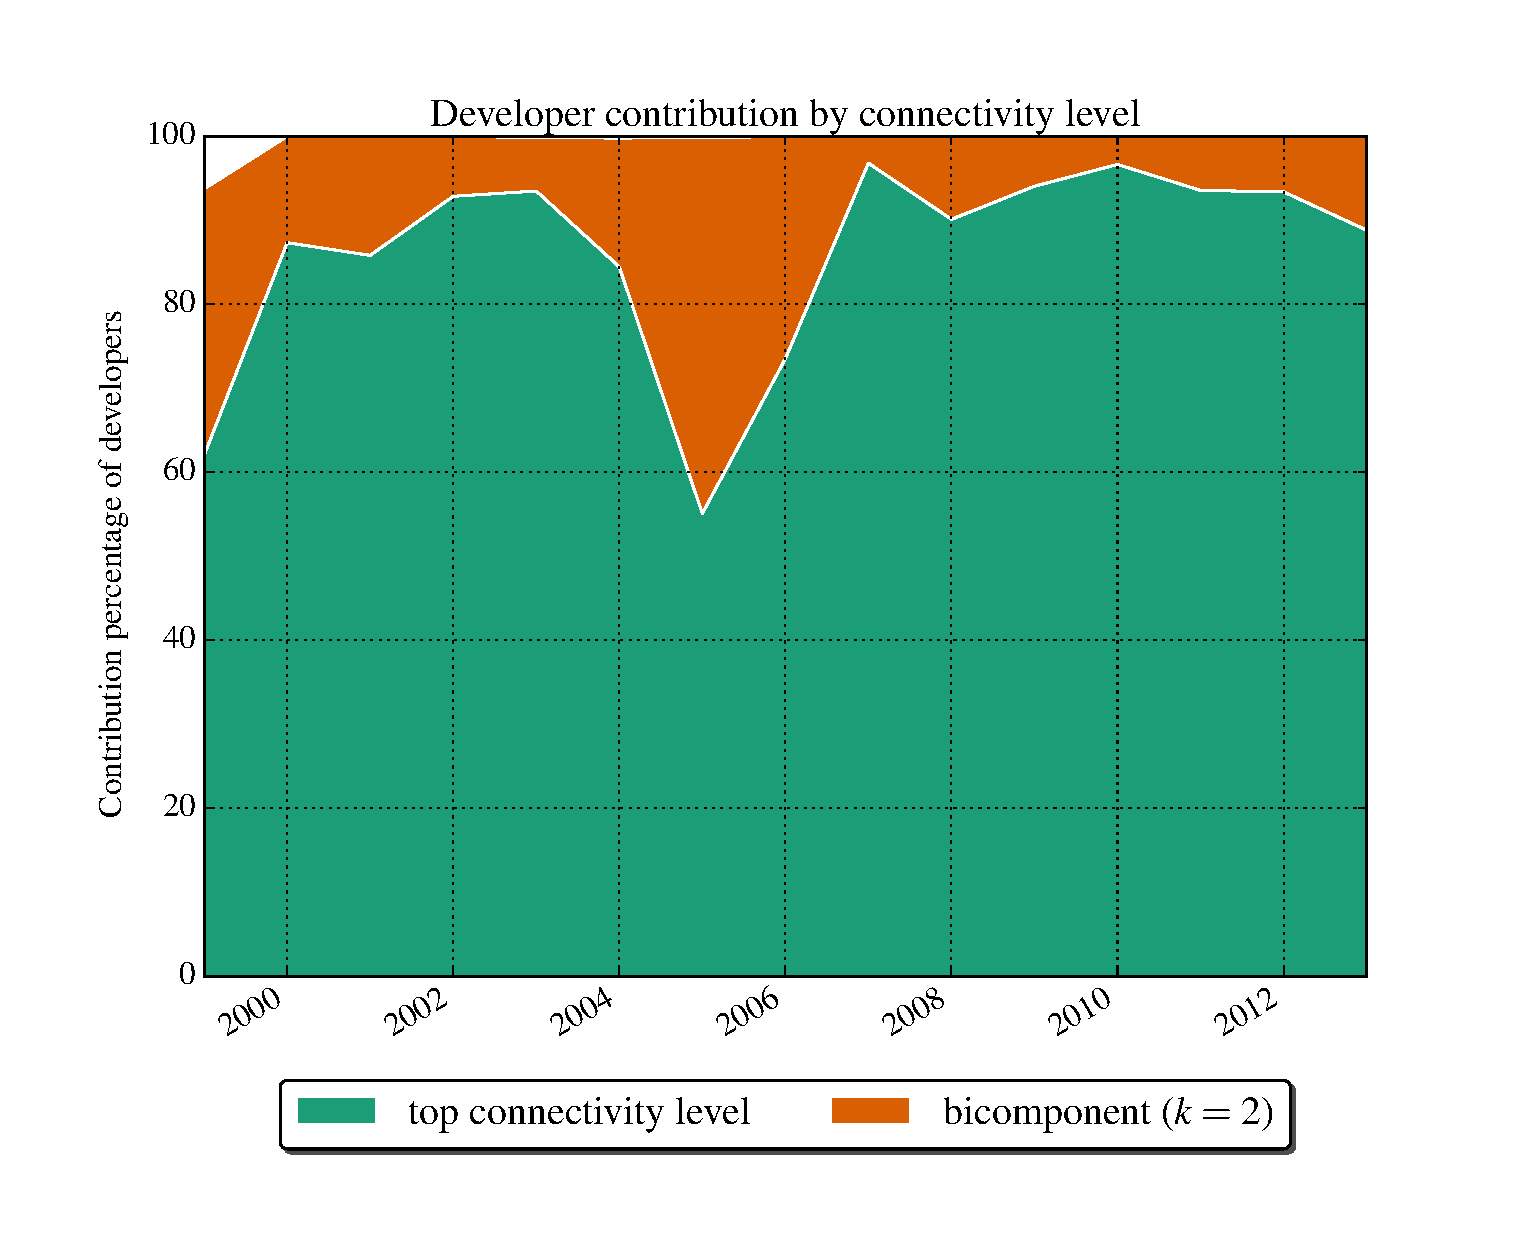
\includegraphics[scale=0.2]{../../figures/evolution_connectivity_python_years}
}
\label{fig:contributions}
\caption[Python: Evolution of connectivity levels and contributions.]{Evolution of the percentage of developers by connectivity level (left) and evolution of the percentage of contributions by developers by connectivity levels (right) in the Python project. The green surface represents the developers in the top connectivity level, that is developers that are part of a $k$-component with maximum $k$. The orange surface represents developers in bicomponents, that is $k$-components with $k=2$.}
\end{figure}

\end{frame}


\begin{frame}
\frametitle{Analyzing Source Code Contributions and beyond}
\note{From the figures on the previous slide, it is clear that there is a strong correlation between the connectivity level of a developer and her level of contribution to the project.

The hierarchical structure of the cooperation network shapes the volume of contribution of individual developers.}

To further the analysis I used more sophisticated statistical modeling strategies to assess the impact of the connectivity structure in the individual contributions to the project.

\begin{itemize}

\item \textbf{Added source code lines to Python:} Modeled with a panel regression with individual and year fixed effect. The position of the individual developer in the connectivity hierarchy is the second most important independent variable only after Degree Centrality.

\end{itemize}

\pause

\begin{block}{Potential endogenity problems of the previous model}
There is a relation between the dependent variable and the network metrics (independent variables) because the cooperation networks are build precisely based on contributions to the project.
\end{block}

\begin{itemize}

\item \textbf{Number of accepted \textit{Python Enhancement Proposals} (PEP):} Modeled with a zero inflated negative binomial. PEPs are design documents that define the language; are thus contributions not directly related to the cooperation networks. Being part of the top connectivity level is also the second most important independent variable, this time only after developer's tenure (in years).

\end{itemize}


\end{frame}



\begin{frame}
\frametitle{The Hierarchical Structure of FOSS projects}

Free and Open Source Software (FOSS) communities have attracted a lot of attention from researchers. Academic efforts took mainly two directions:

\begin{columns}[c]
\begin{column}{0.5\textwidth}
\begin{block}{Reconcile with neoclassical economy}
\begin{itemize}
\item Mainly focused on the individual motivations of the participants. What is usually referred as ``microfundaments''.
\item Trying to explain motivations in terms of of rational self-interested individuals to match the dominant economic accounts.
\end{itemize}
\end{block}
\end{column}

\pause

\begin{column}{0.5\textwidth}

\begin{block}{Uncritically celebratory and a bit naive}
\begin{itemize}
\item Supported the ethical stand that valued more cooperation and reciprocity than competition and self-interest.
\item Assumed that FOSS communities are composed by loosely organized individuals with a very flat or nonexistent hierarchy among them.
\end{itemize}
\end{block}
\end{column}
\end{columns}

\pause

%\vspace{0.5cm}

\begin{block}{Well established empirical fact about FOSS projects}
\begin{itemize}
\item Only few of the participants account for the lion's share of the work done.
%\item The deep contribution inequalities may mean that these projects follow the ``iron law of the oligarchy'' \citep{shaw:2014}.
%\item I propose that one of the central characteristics of FOSS projects is their high ratio of turnover in key hierarchical positions.
\end{itemize}
\end{block}

\end{frame}


\begin{frame}
\frametitle{Empirical Analysis of Individual Contributions}

\note{The informal structure emerging from the patterns of cooperation among individuals in a FOSS project is quite hierarchical because reflects the fact that only few individuals are responsible for most contributions to the project.}

\begin{block}{Longitudinal Analysis of the Social Structure of FOSS projects}
The social structure of a community are the patterns of relations established among individual participants in the production process. But I do not limit the analysis to one point in time; I analyze its evolution.
\end{block}

\pause


\begin{columns}[c]
\begin{column}{0.5\textwidth}
\begin{block}{Puzzle: FOSS projects as Oligarchies?}
\citet{michels:1915} ``iron law of oligarchy'' states that organizations tend towards oligarchy as they grow, even if democracy and participation are part of their core goals.
\end{block}
\end{column}

\begin{column}{0.5\textwidth}
\begin{block}{FOSS projects as Open Elites}
The continuous renewal of the people that does most of the work is a key mechanism to explain how FOSS projects can thrive and success through time.
\end{block}
\end{column}
\end{columns}

\pause

\begin{block}{Longitudinal analysis}
If we analyze a FOSS project in a concrete point of time, only a very small fraction of the participants are the ones that actually do the lion's share of contributions, as previous empirical research has shown.

However if we analyze the evolution of contributions longitudinally, we find that the persons that contribute the most change through time.
\end{block}

\end{frame}



\begin{frame}
\frametitle{Cooperation Networks' Connectivity Hierarchies as Open Elites}

The ratio of renewal of individuals at the top of the connectivity hierarchy is quite fast, which characterizes the CPython project as an open elite.

\begin{figure}
\centering
\vspace{-0.2cm}
\hspace{-0.8cm}
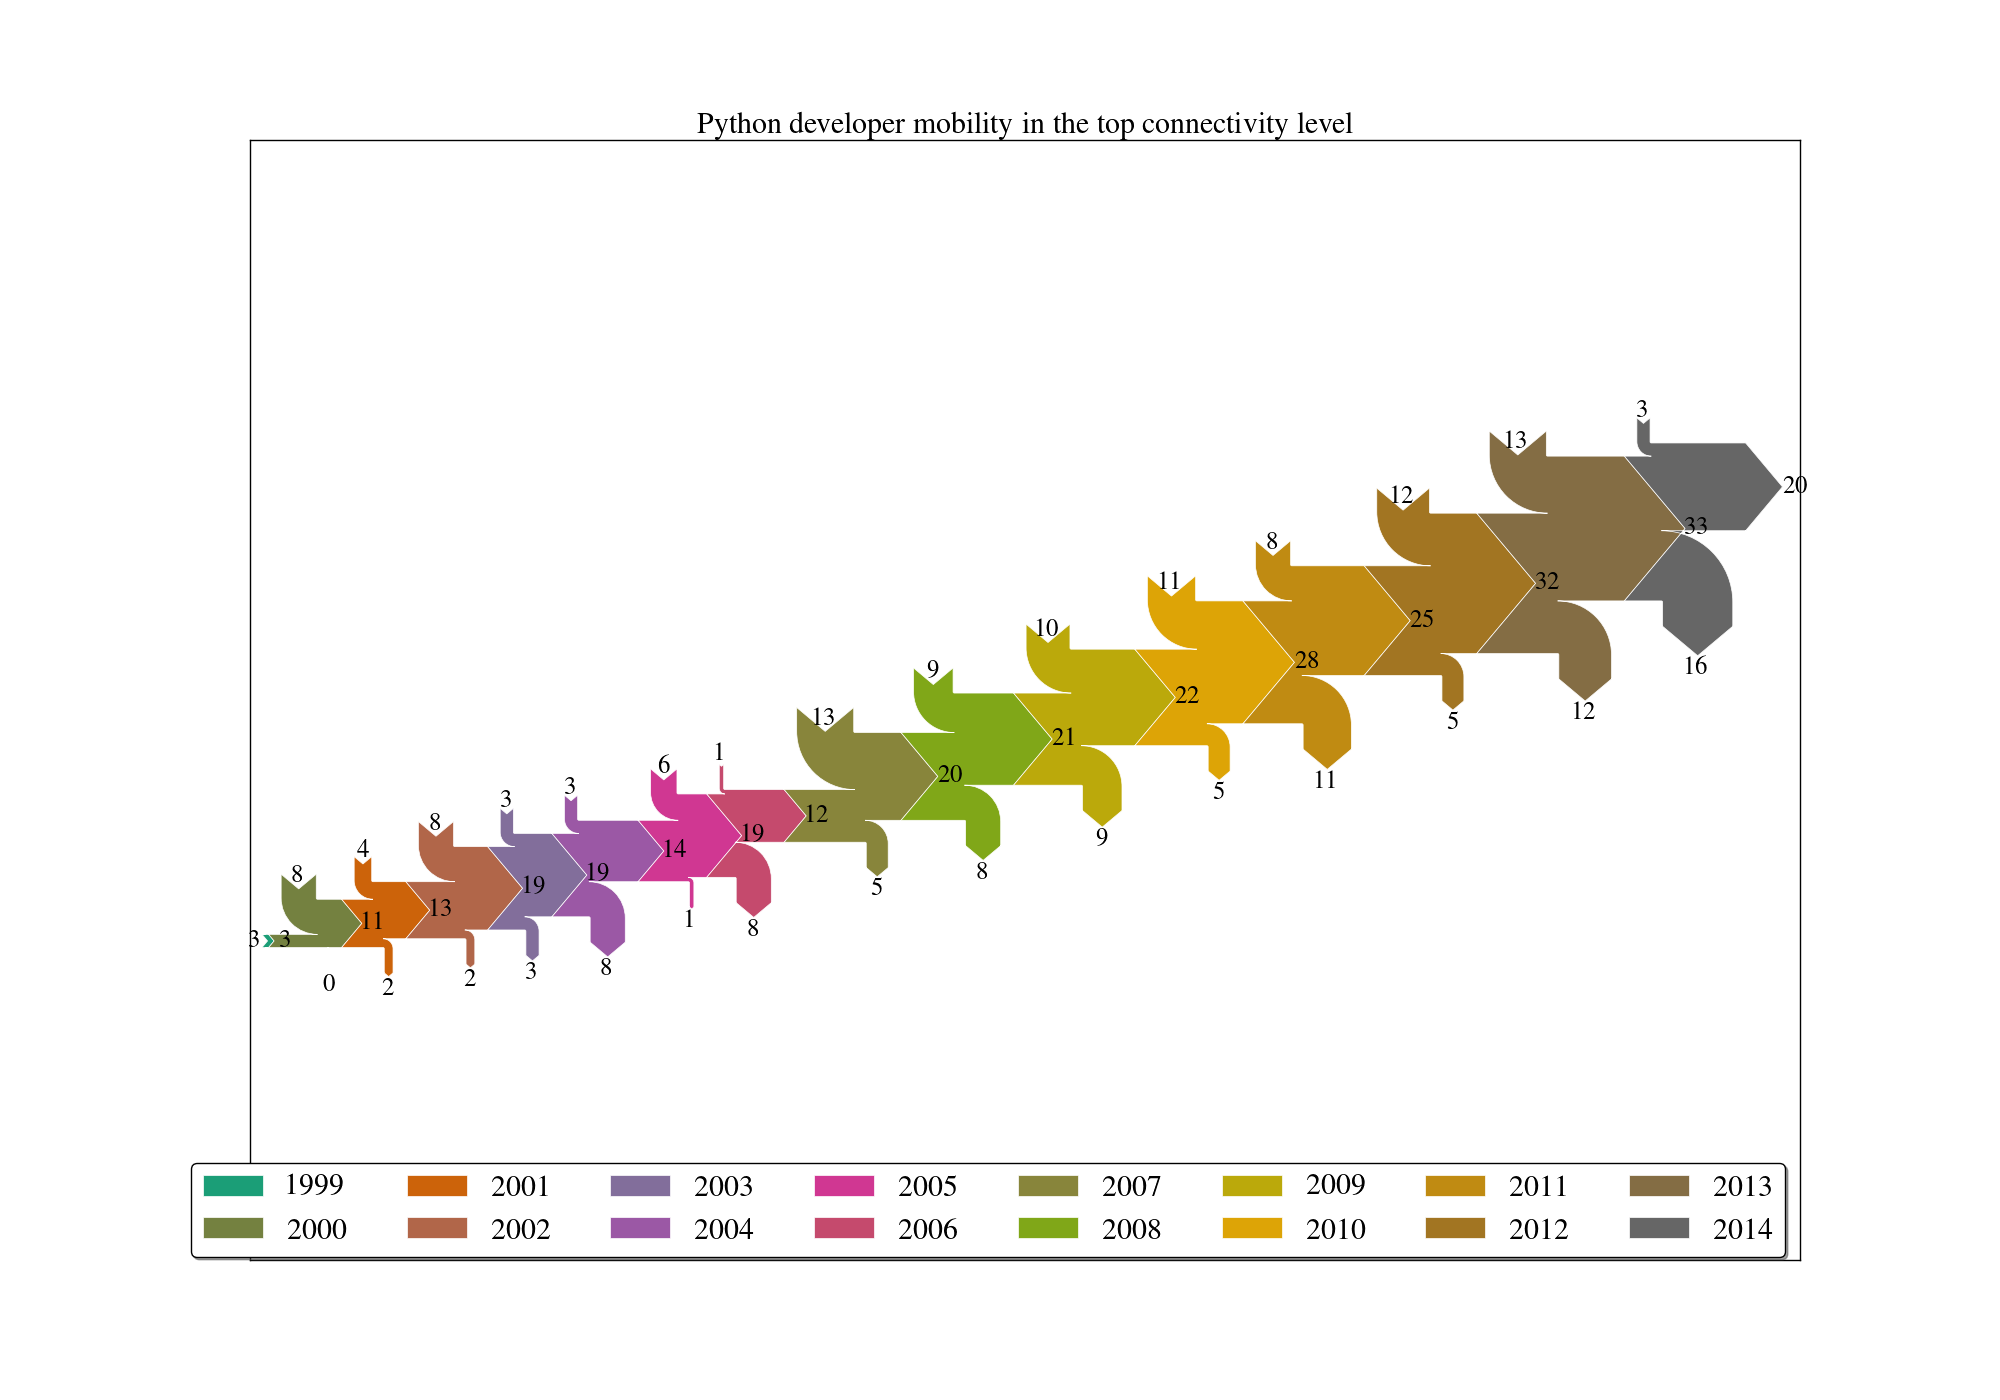
\includegraphics[scale=0.23]{../../figures/sankey_mobility_python_years}
\caption{Sankey diagram of Python developer mobility at the top connectivity level.}
\end{figure}

\end{frame}


\begin{frame}
\frametitle{Modeling robustness of Cooperation Networks}

\begin{columns}[c]
\begin{column}{0.5\textwidth}
\begin{block}{Usual measures of robustness}
\begin{itemize}
%\item Perform simulations \citep{albert:2000} of:
\item Failures: remove nodes at random and see how this affects the size of the giant component.  
\item Attacks: remove nodes incrementally starting for the ones with higher degree.
\end{itemize}
\end{block}
\end{column}

\pause

\begin{column}{0.5\textwidth}

\begin{block}{My approach: Survival analysis}
\begin{itemize}
%\item Origin in medicine: Used to model lifespans of ill individuals.
\item I model active life of a developer as the period that this developer is contributing to the project.
\item I consider a developer ``dead'' when she no longer contributes to the project.
\end{itemize}
\end{block}
\end{column}
\end{columns}

\pause

\begin{block}{Cox proportional hazards model}
The position of an individual in the connectivity hierarchy impacts significantly their median active life in the project.

\begin{itemize}
\item Being part of the top connectivity level decreases the yearly hazard of leaving the project by 77\%.
\item Also an increment of one connectivity level decreases the yearly hazard of leaving the project by 26\%.
\end{itemize}
\end{block}

\pause

\begin{block}{Estimating the survival function with the Kaplan-Meier estimator}
\begin{columns}[c]
\begin{column}{0.2\textwidth}
$$
\hat{S}(t) = \prod_{t_i < t} \frac{n_i - d_i}{n_i}
$$
\end{column}

\begin{column}{0.7\textwidth}
where $d_i$ are the number of ``death events'' at time $t$ and $n_i$ is the number of subjects at risk of death at time $t$. 
\end{column}
\end{columns}
\end{block}

\end{frame}


\begin{frame}
\frametitle{Modeling robustness as median active live of individuals in the project}

\begin{figure}
\centering
\subfloat[Survival Function for all developers]{
\label{fig:survival_all}
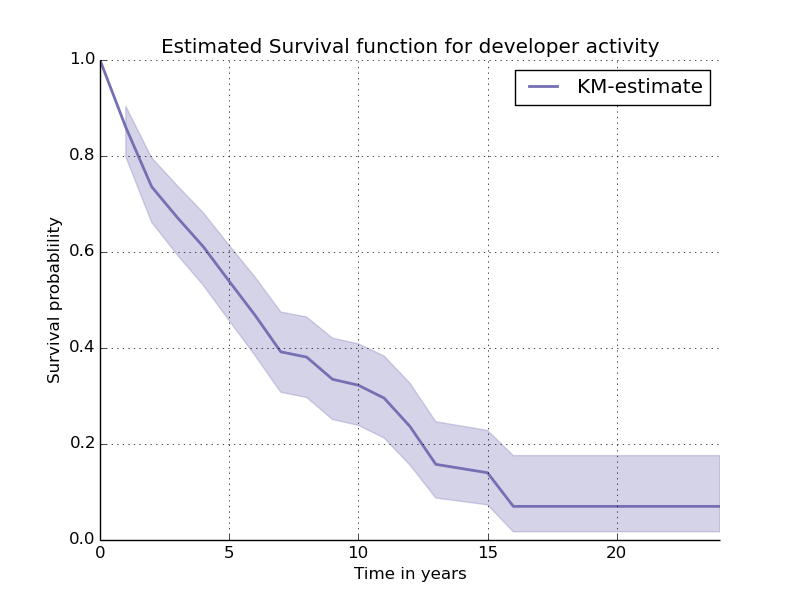
\includegraphics[scale=0.24]{../../figures/survival_all}
}
\hspace{.01in}
\subfloat[Survival Function for developers in the top connectivity level]{
\label{fig:survival_groups}
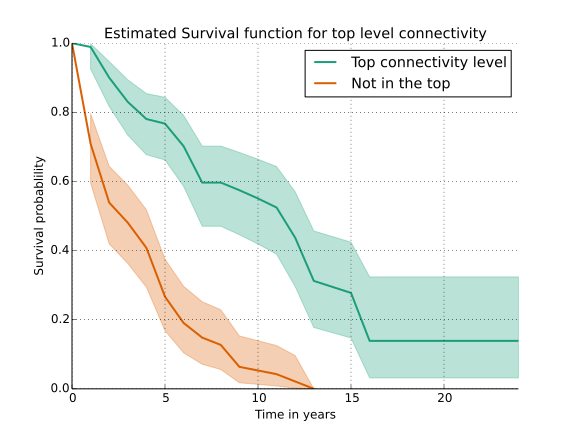
\includegraphics[scale=0.24]{../../figures/survival_top}
}
\label{fig:survival}
\caption[Survival function using the Kaplan-Meier estimate.]{Estimation of the survival function using the Kaplan-Meier estimate. The median survival time of a developer in the community, defined as the point in time where on average half of the population has abandoned the community, is 6 years if I consider all developers (left). But if I consider separately the developers in the top level of the connectivity hierarchy (right), their median survival time is 12 years; but only 3 years for the developers that are not on the top of the connectivity hierarchy.}
\end{figure}

\end{frame}

\section{Conclusions}

\begin{frame}
\frametitle{Conclusions}

\begin{itemize}

%\item \textbf{Cooperation Networks:} A meso level approach to large scale cooperation focused on the patterns of relations that direct producers establish between them in knowledge intensive production processes.

\item The nested structure of $k$-components nicely captures the \textbf{hierarchy in the patterns of relations} that individual contributors establish when working together.

\begin{itemize}
\item reflects the empirically well established fact that in FOSS projects only a small fraction of the developers account for most of the contributions.

\item refutes the naive views of early academic accounts that characterized FOSS projects as a flat hierarchy of peers in which every individual does more or less the same.
\end{itemize}

\item \textbf{Cooperation has a structural dimension} because membership in cohesive groups has an important and statistically significative impact on both the volume of individual contributions, and on the median active life of developers.

\item The connectivity structure of these collaborative communities' cooperation networks can be characterized as an \textbf{open elite}, where the top levels of this hierarchy are filled with new individuals at a high pace. 

\item This feature is \textbf{key for understanding the mechanisms and dynamics} that make FOSS communities able to develop long term projects, with high individual turnover, and yet achieve high impact and coherent results as a result of large scale cooperation.

\end{itemize}

\end{frame}




\begin{frame}[label=biblio]
\frametitle{References}
You can download the slides from: 
\begin{small}
\href{https://github.com/jtorrents/thesis/blob/master/presentations/pydata_bcn/cpython_code_contributions.pdf}{https://github.com/jtorrents/thesis/blob/master/presentations/pydata\_bcn/cpython\_code\_contributions.pdf}
% Bibliografia
\bibliographystyle{chicago}
\bibliography{../../thesis.bib}
\end{small}
\end{frame}

\end{document}
